%----------------------------------------------------------------------------------------
%	PACKAGES AND OTHER DOCUMENT CONFIGURATIONS
%----------------------------------------------------------------------------------------

\documentclass[11pt,fleqn]{book} % Default font size and left-justified equations

%----------------------------------------------------------------------------------------

%%%%%%%%%%%%%%%%%%%%%%%%%%%%%%%%%%%%%%%%%
% The Legrand Orange Book
% Structural Definitions File
% Version 2.0 (9/2/15)
%
% Original author:
% Mathias Legrand (legrand.mathias@gmail.com) with modifications by:
% Vel (vel@latextemplates.com)
% 
% This file has been downloaded from:
% http://www.LaTeXTemplates.com
%
% License:
% CC BY-NC-SA 3.0 (http://creativecommons.org/licenses/by-nc-sa/3.0/)
%
%%%%%%%%%%%%%%%%%%%%%%%%%%%%%%%%%%%%%%%%%

%----------------------------------------------------------------------------------------
%	VARIOUS REQUIRED PACKAGES AND CONFIGURATIONS
%----------------------------------------------------------------------------------------

\usepackage[top=3cm,bottom=3cm,left=3cm,right=3cm,headsep=10pt,a4paper]{geometry} % Page margins

\usepackage{graphicx} % Required for including pictures
\graphicspath{{Pictures/}} % Specifies the directory where pictures are stored

\usepackage{lipsum} % Inserts dummy text

\usepackage{tikz} % Required for drawing custom shapes

\usepackage[english]{babel} % English language/hyphenation

\usepackage{enumitem} % Customize lists
\setlist{nolistsep} % Reduce spacing between bullet points and numbered lists

\usepackage{booktabs} % Required for nicer horizontal rules in tables

\usepackage{xcolor} % Required for specifying colors by name
\definecolor{ocre}{RGB}{243,102,25} % Define the orange color used for highlighting throughout the book

%----------------------------------------------------------------------------------------
%	FONTS
%----------------------------------------------------------------------------------------

\usepackage{avant} % Use the Avantgarde font for headings
%\usepackage{times} % Use the Times font for headings
\usepackage{mathptmx} % Use the Adobe Times Roman as the default text font together with math symbols from the Sym­bol, Chancery and Com­puter Modern fonts

\usepackage{microtype} % Slightly tweak font spacing for aesthetics
\usepackage[utf8]{inputenc} % Required for including letters with accents
\usepackage[T1]{fontenc} % Use 8-bit encoding that has 256 glyphs

%----------------------------------------------------------------------------------------
%	BIBLIOGRAPHY AND INDEX
%----------------------------------------------------------------------------------------

\usepackage{csquotes}
\usepackage[style=alphabetic,citestyle=numeric,sorting=nyt,sortcites=true,autopunct=true,autolang=hyphen,hyperref=true,abbreviate=false,backref=true,backend=biber,defernumbers=true]{biblatex}
\addbibresource{bibliography.bib} % BibTeX bibliography file
\defbibheading{bibempty}{}

\usepackage{calc} % For simpler calculation - used for spacing the index letter headings correctly
\usepackage{makeidx} % Required to make an index
\makeindex % Tells LaTeX to create the files required for indexing

%----------------------------------------------------------------------------------------
%	MAIN TABLE OF CONTENTS
%----------------------------------------------------------------------------------------

\usepackage{titletoc} % Required for manipulating the table of contents

\contentsmargin{0cm} % Removes the default margin

% Part text styling
\titlecontents{part}[0cm]
{\addvspace{20pt}\centering\large\bfseries}
{}
{}
{}

% Chapter text styling
\titlecontents{chapter}[1.25cm] % Indentation
{\addvspace{12pt}\large\sffamily\bfseries} % Spacing and font options for chapters
{\color{ocre!60}\contentslabel[\Large\thecontentslabel]{1.25cm}\color{ocre}} % Chapter number
{\color{ocre}}  
{\color{ocre!60}\normalsize\;\titlerule*[.5pc]{.}\;\thecontentspage} % Page number

% Section text styling
\titlecontents{section}[1.25cm] % Indentation
{\addvspace{3pt}\sffamily\bfseries} % Spacing and font options for sections
{\contentslabel[\thecontentslabel]{1.25cm}} % Section number
{}
{\hfill\color{black}\thecontentspage} % Page number
[]

% Subsection text styling
\titlecontents{subsection}[1.25cm] % Indentation
{\addvspace{1pt}\sffamily\small} % Spacing and font options for subsections
{\contentslabel[\thecontentslabel]{1.25cm}} % Subsection number
{}
{\ \titlerule*[.5pc]{.}\;\thecontentspage} % Page number
[]

% List of figures
\titlecontents{figure}[0em]
{\addvspace{-5pt}\sffamily}
{\thecontentslabel\hspace*{1em}}
{}
{\ \titlerule*[.5pc]{.}\;\thecontentspage}
[]

% List of tables
\titlecontents{table}[0em]
{\addvspace{-5pt}\sffamily}
{\thecontentslabel\hspace*{1em}}
{}
{\ \titlerule*[.5pc]{.}\;\thecontentspage}
[]

%----------------------------------------------------------------------------------------
%	MINI TABLE OF CONTENTS IN PART HEADS
%----------------------------------------------------------------------------------------

% Chapter text styling
\titlecontents{lchapter}[0em] % Indenting
{\addvspace{15pt}\large\sffamily\bfseries} % Spacing and font options for chapters
{\color{ocre}\contentslabel[\Large\thecontentslabel]{1.25cm}\color{ocre}} % Chapter number
{}  
{\color{ocre}\normalsize\sffamily\bfseries\;\titlerule*[.5pc]{.}\;\thecontentspage} % Page number

% Section text styling
\titlecontents{lsection}[0em] % Indenting
{\sffamily\small} % Spacing and font options for sections
{\contentslabel[\thecontentslabel]{1.25cm}} % Section number
{}
{}

% Subsection text styling
\titlecontents{lsubsection}[.5em] % Indentation
{\normalfont\footnotesize\sffamily} % Font settings
{}
{}
{}

%----------------------------------------------------------------------------------------
%	PAGE HEADERS
%----------------------------------------------------------------------------------------

\usepackage{fancyhdr} % Required for header and footer configuration

\pagestyle{fancy}
\renewcommand{\chaptermark}[1]{\markboth{\sffamily\normalsize\bfseries\chaptername\ \thechapter.\ #1}{}} % Chapter text font settings
\renewcommand{\sectionmark}[1]{\markright{\sffamily\normalsize\thesection\hspace{5pt}#1}{}} % Section text font settings
\fancyhf{} \fancyhead[LE,RO]{\sffamily\normalsize\thepage} % Font setting for the page number in the header
\fancyhead[LO]{\rightmark} % Print the nearest section name on the left side of odd pages
\fancyhead[RE]{\leftmark} % Print the current chapter name on the right side of even pages
\renewcommand{\headrulewidth}{0.5pt} % Width of the rule under the header
\addtolength{\headheight}{2.5pt} % Increase the spacing around the header slightly
\renewcommand{\footrulewidth}{0pt} % Removes the rule in the footer
\fancypagestyle{plain}{\fancyhead{}\renewcommand{\headrulewidth}{0pt}} % Style for when a plain pagestyle is specified

% Removes the header from odd empty pages at the end of chapters
\makeatletter
\renewcommand{\cleardoublepage}{
\clearpage\ifodd\c@page\else
\hbox{}
\vspace*{\fill}
\thispagestyle{empty}
\newpage
\fi}

%----------------------------------------------------------------------------------------
%	THEOREM STYLES
%----------------------------------------------------------------------------------------

\usepackage{amsmath,amsfonts,amssymb,amsthm} % For math equations, theorems, symbols, etc

\newcommand{\intoo}[2]{\mathopen{]}#1\,;#2\mathclose{[}}
\newcommand{\ud}{\mathop{\mathrm{{}d}}\mathopen{}}
\newcommand{\intff}[2]{\mathopen{[}#1\,;#2\mathclose{]}}
\newtheorem{notation}{Notation}[chapter]

% Boxed/framed environments
\newtheoremstyle{ocrenumbox}% % Theorem style name
{0pt}% Space above
{0pt}% Space below
{\normalfont}% % Body font
{}% Indent amount
{\small\bf\sffamily\color{ocre}}% % Theorem head font
{\;}% Punctuation after theorem head
{0.25em}% Space after theorem head
{\small\sffamily\color{ocre}\thmname{#1}\nobreakspace\thmnumber{\@ifnotempty{#1}{}\@upn{#2}}% Theorem text (e.g. Theorem 2.1)
\thmnote{\nobreakspace\the\thm@notefont\sffamily\bfseries\color{black}---\nobreakspace#3.}} % Optional theorem note
\renewcommand{\qedsymbol}{$\blacksquare$}% Optional qed square

\newtheoremstyle{blacknumex}% Theorem style name
{5pt}% Space above
{5pt}% Space below
{\normalfont}% Body font
{} % Indent amount
{\small\bf\sffamily}% Theorem head font
{\;}% Punctuation after theorem head
{0.25em}% Space after theorem head
{\small\sffamily{\tiny\ensuremath{\blacksquare}}\nobreakspace\thmname{#1}\nobreakspace\thmnumber{\@ifnotempty{#1}{}\@upn{#2}}% Theorem text (e.g. Theorem 2.1)
\thmnote{\nobreakspace\the\thm@notefont\sffamily\bfseries---\nobreakspace#3.}}% Optional theorem note

\newtheoremstyle{blacknumbox} % Theorem style name
{0pt}% Space above
{0pt}% Space below
{\normalfont}% Body font
{}% Indent amount
{\small\bf\sffamily}% Theorem head font
{\;}% Punctuation after theorem head
{0.25em}% Space after theorem head
{\small\sffamily\thmname{#1}\nobreakspace\thmnumber{\@ifnotempty{#1}{}\@upn{#2}}% Theorem text (e.g. Theorem 2.1)
\thmnote{\nobreakspace\the\thm@notefont\sffamily\bfseries---\nobreakspace#3.}}% Optional theorem note

% Non-boxed/non-framed environments
\newtheoremstyle{ocrenum}% % Theorem style name
{5pt}% Space above
{5pt}% Space below
{\normalfont}% % Body font
{}% Indent amount
{\small\bf\sffamily\color{ocre}}% % Theorem head font
{\;}% Punctuation after theorem head
{0.25em}% Space after theorem head
{\small\sffamily\color{ocre}\thmname{#1}\nobreakspace\thmnumber{\@ifnotempty{#1}{}\@upn{#2}}% Theorem text (e.g. Theorem 2.1)
\thmnote{\nobreakspace\the\thm@notefont\sffamily\bfseries\color{black}---\nobreakspace#3.}} % Optional theorem note
\renewcommand{\qedsymbol}{$\blacksquare$}% Optional qed square
\makeatother

% Defines the theorem text style for each type of theorem to one of the three styles above
\newcounter{dummy} 
\numberwithin{dummy}{section}
\theoremstyle{ocrenumbox}
\newtheorem{theoremeT}[dummy]{Theorem}
\newtheorem{problem}{Problem}[chapter]
\newtheorem{exerciseT}{Exercise}[chapter]
\theoremstyle{blacknumex}
\newtheorem{exampleT}{Example}[chapter]
\theoremstyle{blacknumbox}
\newtheorem{vocabulary}{Vocabulary}[chapter]
\newtheorem{definitionT}{Definition}[section]
\newtheorem{corollaryT}[dummy]{Corollary}
\theoremstyle{ocrenum}
\newtheorem{proposition}[dummy]{Proposition}

%----------------------------------------------------------------------------------------
%	DEFINITION OF COLORED BOXES
%----------------------------------------------------------------------------------------

\RequirePackage[framemethod=default]{mdframed} % Required for creating the theorem, definition, exercise and corollary boxes

% Theorem box
\newmdenv[skipabove=7pt,
skipbelow=7pt,
backgroundcolor=black!5,
linecolor=ocre,
innerleftmargin=5pt,
innerrightmargin=5pt,
innertopmargin=5pt,
leftmargin=0cm,
rightmargin=0cm,
innerbottommargin=5pt]{tBox}

% Exercise box	  
\newmdenv[skipabove=7pt,
skipbelow=7pt,
rightline=false,
leftline=true,
topline=false,
bottomline=false,
backgroundcolor=ocre!10,
linecolor=ocre,
innerleftmargin=5pt,
innerrightmargin=5pt,
innertopmargin=5pt,
innerbottommargin=5pt,
leftmargin=0cm,
rightmargin=0cm,
linewidth=4pt]{eBox}	

% Definition box
\newmdenv[skipabove=7pt,
skipbelow=7pt,
rightline=false,
leftline=true,
topline=false,
bottomline=false,
linecolor=ocre,
innerleftmargin=5pt,
innerrightmargin=5pt,
innertopmargin=0pt,
leftmargin=0cm,
rightmargin=0cm,
linewidth=4pt,
innerbottommargin=0pt]{dBox}	

% Corollary box
\newmdenv[skipabove=7pt,
skipbelow=7pt,
rightline=false,
leftline=true,
topline=false,
bottomline=false,
linecolor=gray,
backgroundcolor=black!5,
innerleftmargin=5pt,
innerrightmargin=5pt,
innertopmargin=5pt,
leftmargin=0cm,
rightmargin=0cm,
linewidth=4pt,
innerbottommargin=5pt]{cBox}

% Creates an environment for each type of theorem and assigns it a theorem text style from the "Theorem Styles" section above and a colored box from above
\newenvironment{theorem}{\begin{tBox}\begin{theoremeT}}{\end{theoremeT}\end{tBox}}
\newenvironment{exercise}{\begin{eBox}\begin{exerciseT}}{\hfill{\color{ocre}\tiny\ensuremath{\blacksquare}}\end{exerciseT}\end{eBox}}				  
\newenvironment{definition}{\begin{dBox}\begin{definitionT}}{\end{definitionT}\end{dBox}}	
\newenvironment{example}{\begin{exampleT}}{\hfill{\tiny\ensuremath{\blacksquare}}\end{exampleT}}		
\newenvironment{corollary}{\begin{cBox}\begin{corollaryT}}{\end{corollaryT}\end{cBox}}	

%----------------------------------------------------------------------------------------
%	REMARK ENVIRONMENT
%----------------------------------------------------------------------------------------

\newenvironment{remark}{\par\vspace{10pt}\small % Vertical white space above the remark and smaller font size
\begin{list}{}{
\leftmargin=35pt % Indentation on the left
\rightmargin=25pt}\item\ignorespaces % Indentation on the right
\makebox[-2.5pt]{\begin{tikzpicture}[overlay]
\node[draw=ocre!60,line width=1pt,circle,fill=ocre!25,font=\sffamily\bfseries,inner sep=2pt,outer sep=0pt] at (-15pt,0pt){\textcolor{ocre}{R}};\end{tikzpicture}} % Orange R in a circle
\advance\baselineskip -1pt}{\end{list}\vskip5pt} % Tighter line spacing and white space after remark

%----------------------------------------------------------------------------------------
%	SECTION NUMBERING IN THE MARGIN
%----------------------------------------------------------------------------------------

\makeatletter
\renewcommand{\@seccntformat}[1]{\llap{\textcolor{ocre}{\csname the#1\endcsname}\hspace{1em}}}                    
\renewcommand{\section}{\@startsection{section}{1}{\z@}
{-4ex \@plus -1ex \@minus -.4ex}
{1ex \@plus.2ex }
{\normalfont\large\sffamily\bfseries}}
\renewcommand{\subsection}{\@startsection {subsection}{2}{\z@}
{-3ex \@plus -0.1ex \@minus -.4ex}
{0.5ex \@plus.2ex }
{\normalfont\sffamily\bfseries}}
\renewcommand{\subsubsection}{\@startsection {subsubsection}{3}{\z@}
{-2ex \@plus -0.1ex \@minus -.2ex}
{.2ex \@plus.2ex }
{\normalfont\small\sffamily\bfseries}}                        
\renewcommand\paragraph{\@startsection{paragraph}{4}{\z@}
{-2ex \@plus-.2ex \@minus .2ex}
{.1ex}
{\normalfont\small\sffamily\bfseries}}

%----------------------------------------------------------------------------------------
%	PART HEADINGS
%----------------------------------------------------------------------------------------

% numbered part in the table of contents
\newcommand{\@mypartnumtocformat}[2]{%
\setlength\fboxsep{0pt}%
\noindent\colorbox{ocre!20}{\strut\parbox[c][.7cm]{\ecart}{\color{ocre!70}\Large\sffamily\bfseries\centering#1}}\hskip\esp\colorbox{ocre!40}{\strut\parbox[c][.7cm]{\linewidth-\ecart-\esp}{\Large\sffamily\centering#2}}}%
%%%%%%%%%%%%%%%%%%%%%%%%%%%%%%%%%%
% unnumbered part in the table of contents
\newcommand{\@myparttocformat}[1]{%
\setlength\fboxsep{0pt}%
\noindent\colorbox{ocre!40}{\strut\parbox[c][.7cm]{\linewidth}{\Large\sffamily\centering#1}}}%
%%%%%%%%%%%%%%%%%%%%%%%%%%%%%%%%%%
\newlength\esp
\setlength\esp{4pt}
\newlength\ecart
\setlength\ecart{1.2cm-\esp}
\newcommand{\thepartimage}{}%
\newcommand{\partimage}[1]{\renewcommand{\thepartimage}{#1}}%
\def\@part[#1]#2{%
\ifnum \c@secnumdepth >-2\relax%
\refstepcounter{part}%
\addcontentsline{toc}{part}{\texorpdfstring{\protect\@mypartnumtocformat{\thepart}{#1}}{\partname~\thepart\ ---\ #1}}
\else%
\addcontentsline{toc}{part}{\texorpdfstring{\protect\@myparttocformat{#1}}{#1}}%
\fi%
\startcontents%
\markboth{}{}%
{\thispagestyle{empty}%
\begin{tikzpicture}[remember picture,overlay]%
\node at (current page.north west){\begin{tikzpicture}[remember picture,overlay]%	
\fill[ocre!20](0cm,0cm) rectangle (\paperwidth,-\paperheight);
\node[anchor=north] at (4cm,-3.25cm){\color{ocre!40}\fontsize{220}{100}\sffamily\bfseries\@Roman\c@part}; 
\node[anchor=south east] at (\paperwidth-1cm,-\paperheight+1cm){\parbox[t][][t]{8.5cm}{
\printcontents{l}{0}{\setcounter{tocdepth}{1}}%
}};
\node[anchor=north east] at (\paperwidth-1.5cm,-3.25cm){\parbox[t][][t]{15cm}{\strut\raggedleft\color{white}\fontsize{30}{30}\sffamily\bfseries#2}};
\end{tikzpicture}};
\end{tikzpicture}}%
\@endpart}
\def\@spart#1{%
\startcontents%
\phantomsection
{\thispagestyle{empty}%
\begin{tikzpicture}[remember picture,overlay]%
\node at (current page.north west){\begin{tikzpicture}[remember picture,overlay]%	
\fill[ocre!20](0cm,0cm) rectangle (\paperwidth,-\paperheight);
\node[anchor=north east] at (\paperwidth-1.5cm,-3.25cm){\parbox[t][][t]{15cm}{\strut\raggedleft\color{white}\fontsize{30}{30}\sffamily\bfseries#1}};
\end{tikzpicture}};
\end{tikzpicture}}
\addcontentsline{toc}{part}{\texorpdfstring{%
\setlength\fboxsep{0pt}%
\noindent\protect\colorbox{ocre!40}{\strut\protect\parbox[c][.7cm]{\linewidth}{\Large\sffamily\protect\centering #1\quad\mbox{}}}}{#1}}%
\@endpart}
\def\@endpart{\vfil\newpage
\if@twoside
\if@openright
\null
\thispagestyle{empty}%
\newpage
\fi
\fi
\if@tempswa
\twocolumn
\fi}

%----------------------------------------------------------------------------------------
%	CHAPTER HEADINGS
%----------------------------------------------------------------------------------------

% A switch to conditionally include a picture, implemented by  Christian Hupfer
\newif\ifusechapterimage
\usechapterimagetrue
\newcommand{\thechapterimage}{}%
\newcommand{\chapterimage}[1]{\ifusechapterimage\renewcommand{\thechapterimage}{#1}\fi}%
\def\@makechapterhead#1{%
{\parindent \z@ \raggedright \normalfont
\ifnum \c@secnumdepth >\m@ne
\if@mainmatter
\begin{tikzpicture}[remember picture,overlay]
\node at (current page.north west)
{\begin{tikzpicture}[remember picture,overlay]
\node[anchor=north west,inner sep=0pt] at (0,0) {\ifusechapterimage\includegraphics[width=\paperwidth]{\thechapterimage}\fi};
\draw[anchor=west] (\Gm@lmargin,-9cm) node [line width=2pt,rounded corners=15pt,draw=ocre,fill=white,fill opacity=0.5,inner sep=15pt]{\strut\makebox[22cm]{}};
\draw[anchor=west] (\Gm@lmargin+.3cm,-9cm) node {\huge\sffamily\bfseries\color{black}\thechapter. #1\strut};
\end{tikzpicture}};
\end{tikzpicture}
\else
\begin{tikzpicture}[remember picture,overlay]
\node at (current page.north west)
{\begin{tikzpicture}[remember picture,overlay]
\node[anchor=north west,inner sep=0pt] at (0,0) {\ifusechapterimage\includegraphics[width=\paperwidth]{\thechapterimage}\fi};
\draw[anchor=west] (\Gm@lmargin,-9cm) node [line width=2pt,rounded corners=15pt,draw=ocre,fill=white,fill opacity=0.5,inner sep=15pt]{\strut\makebox[22cm]{}};
\draw[anchor=west] (\Gm@lmargin+.3cm,-9cm) node {\huge\sffamily\bfseries\color{black}#1\strut};
\end{tikzpicture}};
\end{tikzpicture}
\fi\fi\par\vspace*{270\p@}}}

%-------------------------------------------

\def\@makeschapterhead#1{%
\begin{tikzpicture}[remember picture,overlay]
\node at (current page.north west)
{\begin{tikzpicture}[remember picture,overlay]
\node[anchor=north west,inner sep=0pt] at (0,0) {\ifusechapterimage\includegraphics[width=\paperwidth]{\thechapterimage}\fi};
\draw[anchor=west] (\Gm@lmargin,-9cm) node [line width=2pt,rounded corners=15pt,draw=ocre,fill=white,fill opacity=0.5,inner sep=15pt]{\strut\makebox[22cm]{}};
\draw[anchor=west] (\Gm@lmargin+.3cm,-9cm) node {\huge\sffamily\bfseries\color{black}#1\strut};
\end{tikzpicture}};
\end{tikzpicture}
\par\vspace*{270\p@}}
\makeatother

%----------------------------------------------------------------------------------------
%	HYPERLINKS IN THE DOCUMENTS
%----------------------------------------------------------------------------------------

\usepackage{hyperref}
\hypersetup{hidelinks,colorlinks=false,breaklinks=true,urlcolor= ocre,bookmarksopen=false,pdftitle={Title},pdfauthor={Author}}
\usepackage{bookmark}
\bookmarksetup{
open,
numbered,
addtohook={%
\ifnum\bookmarkget{level}=0 % chapter
\bookmarksetup{bold}%
\fi
\ifnum\bookmarkget{level}=-1 % part
\bookmarksetup{color=ocre,bold}%
\fi
}
}
 % Insert the commands.tex file which contains the majority of the structure behind the template

%----------------------------------------------------------------------------------------

% Extra packages
\usepackage{setspace}
\usepackage{nicematrix}
\usepackage{pgfplots}
\pgfplotsset{compat=1.18}
\usepackage{mathrsfs}
\usepackage{tikz-3dplot}
\usepackage{cancel}
\usepackage{circledsteps}
\tdplotsetmaincoords{60}{115}
% Colors
\definecolor{LightBlue}{rgb}{0.0, 0.64, 1.0}
\definecolor{DarkGreen}{rgb}{0.31, 0.54, 0.30}
% Font types
\DeclareTextFontCommand{\bred}{\color{red}\bfseries} % Bold and red
\DeclareTextFontCommand{\itblue}{\color{LightBlue}\itshape} % Italic and blue
\DeclareTextFontCommand{\term}{\color{orange}\itshape} % Italic and blue
% Math settings
\everymath{\displaystyle}

\usetikzlibrary{external}
\tikzexternalize[prefix=figures/]
\tikzset{external/only named=true}


%----------------------------------------------------------------------------------------

\begin{document}

%----------------------------------------------------------------------------------------
%	TITLE PAGE
%----------------------------------------------------------------------------------------

\begingroup
\thispagestyle{empty}
\begin{tikzpicture}[remember picture,overlay]
    \coordinate [below=12cm] (midpoint) at (current page.north);
    \node at (current page.north west)
    {\begin{tikzpicture}[remember picture,overlay]
        \node[anchor=north west,inner sep=0pt] at (0,0) {
\includegraphics[width=\paperwidth]{background}}; % Background image
        \draw[anchor=north] (midpoint) node [fill=ocre!30!white,fill opacity=0.6,text opacity=1,inner sep=1cm]{\Huge\centering\bfseries\sffamily\parbox[c][][t]{\paperwidth}{\centering MAT235\\[15pt] % Book title
        {\Large Multivariable Calculus}\\[20pt] % Subtitle
        {\huge Sinan Li}}}; % Author name
    \end{tikzpicture}};
\end{tikzpicture}
\vfill
\endgroup

%----------------------------------------------------------------------------------------
%	COPYRIGHT PAGE
%----------------------------------------------------------------------------------------

\newpage
~\vfill
\thispagestyle{empty}

\noindent Copyright \copyright\ 2022 Sinan Li\\ % Copyright notice

\noindent \textsc{Published by Sinan Li}\\ % Publisher

\noindent \textsc{artsci.calendar.utoronto.ca/course/mat235y1}\\ % URL

\noindent Licensed under the Creative Commons Attribution-NonCommercial 3.0 Unported License (the ``License''). You may not use this file except in compliance with the License. You may obtain a copy of the License at \url{http://creativecommons.org/licenses/by-nc/3.0}. Unless required by applicable law or agreed to in writing, software distributed under the License is distributed on an \textsc{``as is'' basis, without warranties or conditions of any kind}, either express or implied. See the License for the specific language governing permissions and limitations under the License.\\ % License information

\noindent \textit{First digital, May 2022} % Printing/edition date

%----------------------------------------------------------------------------------------
%	TABLE OF CONTENTS
%----------------------------------------------------------------------------------------

%\usechapterimagefalse % If you don't want to include a chapter image, use this to toggle images off - it can be enabled later with \usechapterimagetrue

\chapterimage{chapter_head_1.pdf} % Table of contents heading image

\pagestyle{empty} % No headers

\tableofcontents % Print the table of contents itself

\cleardoublepage % Forces the first chapter to start on an odd page so it's on the right

\pagestyle{fancy} % Print headers again


%----------------------------------------------------------------------------------------
%	LECTURE NOES
%----------------------------------------------------------------------------------------

\part{Lecture Notes}

\chapterimage{chapter_head_2.pdf}

\chapter*{Introduction}
\addcontentsline{toc}{chapter}{\textcolor{ocre}{Introduction}}

Parametric equations and polar coordinates. Vectors, vector functions and space curves. Differential and integral calculus of functions of several variables. Line integrals and surface integrals and classic vector calculus theorems. Examples from life sciences and physical science applications.

{~~~}

This is a second-year \bred{Multivariable Calculus} course. The depth of mathematics will be taught at the standard level accessibly to all second-year undergraduate students who has fully finished any first year Introduction to Calculus course. The course will have significant emphasis on computation. In general, theorems will be stated without proofs, but with an indication of the mathematical ideas involved. No emphasis will be put on rigorous mathematic proofs.

\textbf{Requirements}

Any full first-year Introduction to Calculus course is acceptable, preferably with depth taught at the standard level for first-year undergraduate students. Some examples of the courses include, but are not limited to: MAT135/136; MAT137; MAT157; MAT133; There will be a review of key concepts that we need from Linear Algebra at the beginning of the course, so it is not necessary to have any background in linear algebra.

\textbf{Textbook}

\begin{itemize}
    \item Single Variable Calculus: Early Transcendentals, Stewart (8th/9th Edition) \cite{Stewart}
    \item Advanced Calculus, Folland
\end{itemize}

\textbf{The textbooks are optional}, and are not necessary to the course. 

\chapterimage{c1.png}

\chapter{Conic Sections}

\section{Curved Lines}

An equation involving $x$ and $y$ gives a \term{curve}\index{Curved Line} in the plane.

By replacing $x$ with $x - a$, the graph is shifted to the right by $a$. By replacing $y$ with $y - b$, the graph is shifted upward by $b$.

\begin{center}
    \tikzsetnextfilename{c01s01-f01}%
    \begin{tikzpicture}
        \draw[->] (-2.2, 0) -- (2.2, 0) node[right] {$x$};
        \draw[->] (0, -1.2) -- (0, 3.2) node[above] {$y$};

        \draw[thick,blue,domain=-1.5:1.5,smooth] plot (\x,{(\x)^2}) node [above right] {$y = x^2$};
        \draw[thick,red,domain=-0.5:2.5,smooth] plot (\x,{(\x - 1)^2}) node [right] {$y = (x - a)^2$};
        \draw[thick,DarkGreen,domain=-1.5:1.5,smooth] plot (\x,{(\x)^2 + 1}) node [above] {$y - b = x^2$};
    \end{tikzpicture}
\end{center}

\begin{definition}[Parabola]\index{Parabola}
    The \term{parabola} (with vertex) at the origin is defined by $$y = ax^2 \qquad x = by^2$$

    \begin{itemize}
        \item $y = ax^2$ opens up for $a > 0$, and opens down for $a < 0$.
        \item $x = by^2$ opens to the right for $b > 0$, and opens to the left for $b < 0$.
    \end{itemize}
\end{definition}

\begin{center}
    \tikzsetnextfilename{c01s01-f02}%
    \begin{tikzpicture}
        \draw[->] (-2.2, 0) -- (2.2, 0) node[right] {$x$};
        \draw[->] (0, -1.2) -- (0, 3.2) node[above] {$y$};

        \draw[thick,blue,domain=-1.5:1.5,smooth] plot (\x, {(\x)^2}) node [above] {$y = ax^2$};
    \end{tikzpicture}
    \qquad
    \tikzsetnextfilename{c01s01-f03}%
    \begin{tikzpicture}
        \draw[->] (-1.2, 0) -- (3.2, 0) node[right] {$x$};
        \draw[->] (0, -2.2) -- (0, 2.2) node[above] {$y$};

        \draw[thick,blue,domain=0:2.5,smooth] plot (\x, {sqrt(\x)}) node [above] {$x = by^2$};
        \draw[thick,blue,domain=0:2.5,smooth] plot (\x, {-sqrt(\x)});
    \end{tikzpicture}
\end{center}

\begin{definition}[Ellipse]\index{Ellipse}
    The \term{ellipse} (with center) at the origin is defined by $$\left(\frac{x}{a}\right)^2 + \left(\frac{y}{b}\right)^2 = 1$$ with $(a, 0)$ being the right-most point on the $x$-axis, and $(0, b)$ as the top-most point on the $y$-axis.

    When $a = b$, an ellipse becomes a \term{circle}, with $a = b = R$ as the radius of the circle \footnote{$\left(\frac{x}{R}\right)^2 + \left(\frac{y}{R}\right)^2 = 1 \implies x^2 + y^2 = R^2$}.
\end{definition}

\begin{center}
    \tikzsetnextfilename{c01s01-f04}%
    \begin{tikzpicture}
        \draw[->] (-3.2, 0) -- (3.2, 0) node[right] {$x$};
        \draw[->] (0, -1.7) -- (0, 1.7) node[above] {$y$};

        \draw[thick,blue] (0, 0) ellipse (2cm and 1cm);

        \draw[thick,red] (2, 0.25) -- (2, 0) node[below,red] {$a$};
        \draw[thick,red] (0.25, 1) -- (0, 1) node[left,red] {$b$};
    \end{tikzpicture}
\end{center}

\begin{definition}[Hyperbola]\index{Hyperbola}
    The \term{hyperbola} (with center) at the origin is defined by $$\left(\frac{x}{a}\right)^2 - \left(\frac{y}{b}\right)^2 = 1 \qquad \left(\frac{y}{a}\right)^2 - \left(\frac{x}{b}\right)^2 = 1$$

    A hyperbola has 2 curves, and a center line that is not crossed. The 2 curves goes in the opposite direction of the center.
\end{definition}

\begin{center}
    \tikzsetnextfilename{c01s01-f05}%
    \begin{tikzpicture}
        \draw[->] (-2.2, 0) -- (2.2, 0) node[right] {$x$};
        \draw[->] (0, -2.2) -- (0, 2.2) node[above] {$y$};

        \clip(-2, -2) rectangle (2, 2);

        \draw[thick,blue,domain=-0.99:0.99] plot ({( 1+(\x)^2)/(1-(\x)^2)}, {  2 *(\x)/(1-(\x)^2)});
        \draw[thick,blue,domain=-0.99:0.99] plot ({(-1-(\x)^2)/(1-(\x)^2)}, {(-2)*(\x)/(1-(\x)^2)});

        \draw[densely dashed,DarkGreen,domain=-2:2] plot (\x, \x);
        \draw[densely dashed,DarkGreen,domain=-2:2] plot (\x, -\x);
        \node[DarkGreen] at (0,-1) {$y = \frac{b}{a}x$};

        \draw[red] (-1,0.25) -- (-1,0) node[below] {$-|a|$};
        \draw[red] (1,0.25) -- (1,0) node[below] {$|a|$};
        \node[blue] at (0,1.5) {$\displaystyle \left(\frac{x}{a}\right)^2 - \left(\frac{y}{b}\right)^2 = 1$};
    \end{tikzpicture}
\end{center}

Since the right side is positive, and a square is positive, the position of the negative sign determines the direction of the curves.

To determine the direction, we can either set $x = 0$ or $y = 0$. For example, in the case of $x^2 - y^2 = 1$, by setting $x = 0$, we attain $-y^2 = 1$ is impossible, so the vertical line $x = 0$ is the center is never crossed. Thus the 2 curves open towards left and right.

To find the \bred{slant asymptotes} when $x$ and $y$ are both large, change the number $1$ on the right side of the equation to $0$.

{~~~}

The above 3 curves together are sometimes called: \term{Conic Sections}\index{Conic Sections}.

\section{Curved Surfaces}

An equation involving $x$, $y$, and $z$ gives a \term{curved surface}\index{Curved surface} in 3D space. In general, this surface is difficult to imagine and sketch in 3D.

\begin{definition}[3D Sphere]\index{Sphere}
    The \term{3D Sphere} (with center) at the origin with radius $R$ is given by $$x^2 + y^2 + z^2 = R^2$$
\end{definition}

\begin{center} 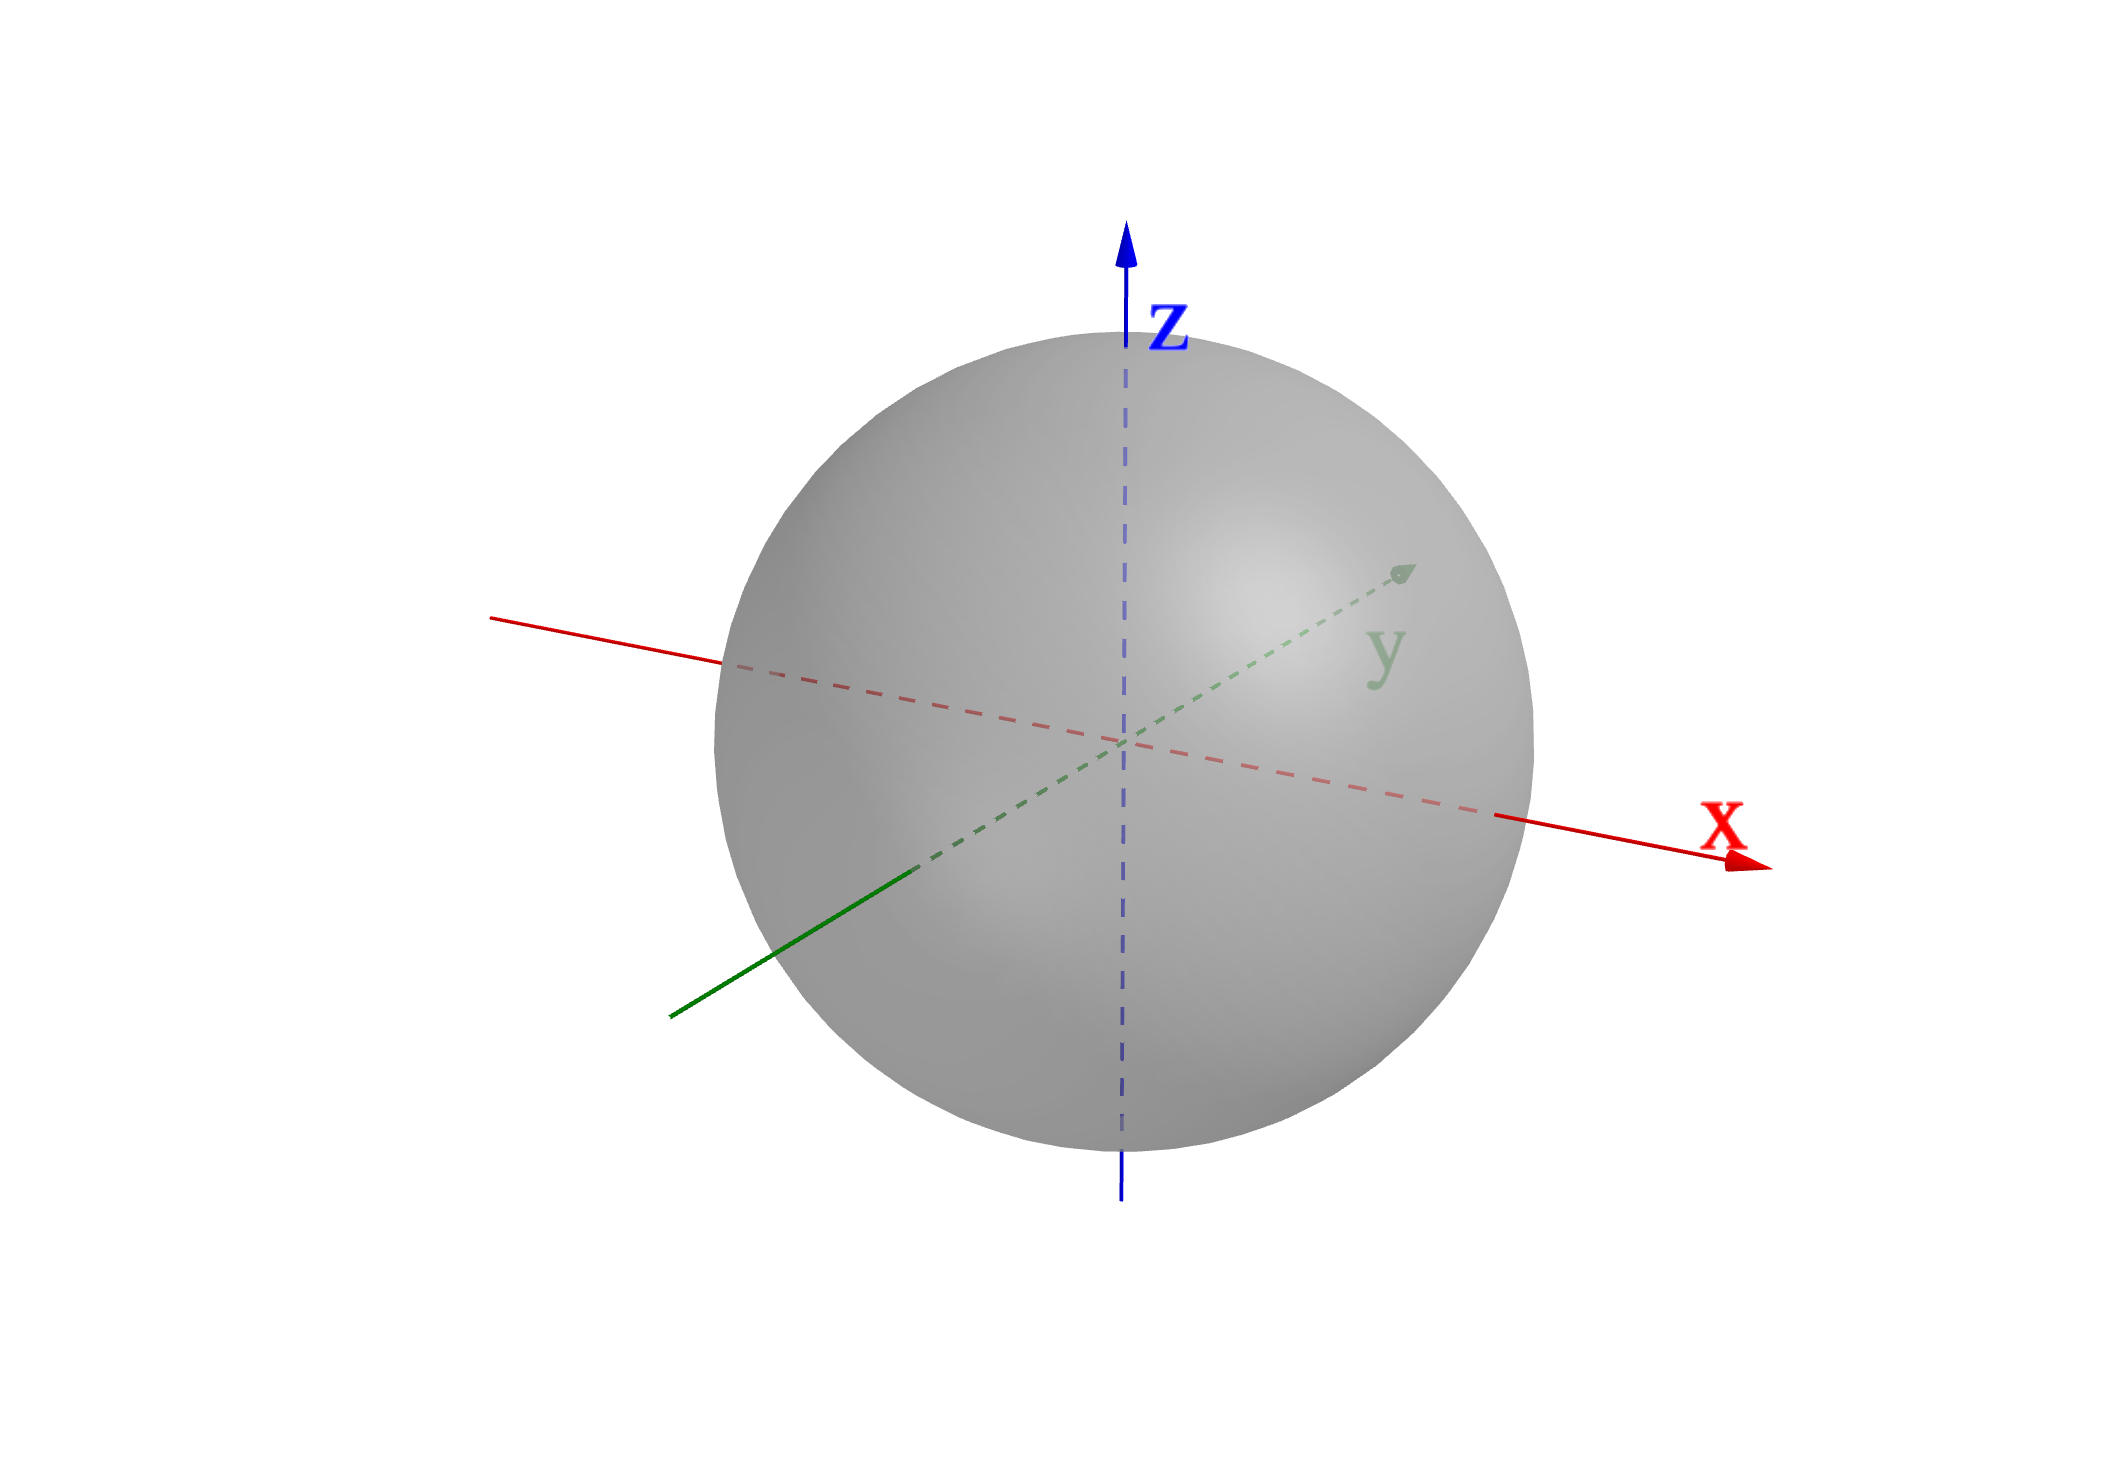
\includegraphics[width=0.5\textwidth]{Plots/sphere.png} \end{center}

\begin{definition}[Ellipsoid]\index{Ellipsoid}
    The 3D \term{ellipsoid} (with center) at the origin is given by $$\left(\frac{x}{a}\right)^2 + \left(\frac{y}{b}\right)^2 + \left(\frac{z}{c}\right)^2 = 1$$

    $(a, 0, 0)$, $(0, b, 0)$, $(0, 0, c)$ are the 3 points on the ellipsoid, similar to the ellipse.

    When $a = b = c$, an ellipsoid becomes a \term{sphere}, with $a = b = c = R$ as the radius.
\end{definition}

\begin{center} 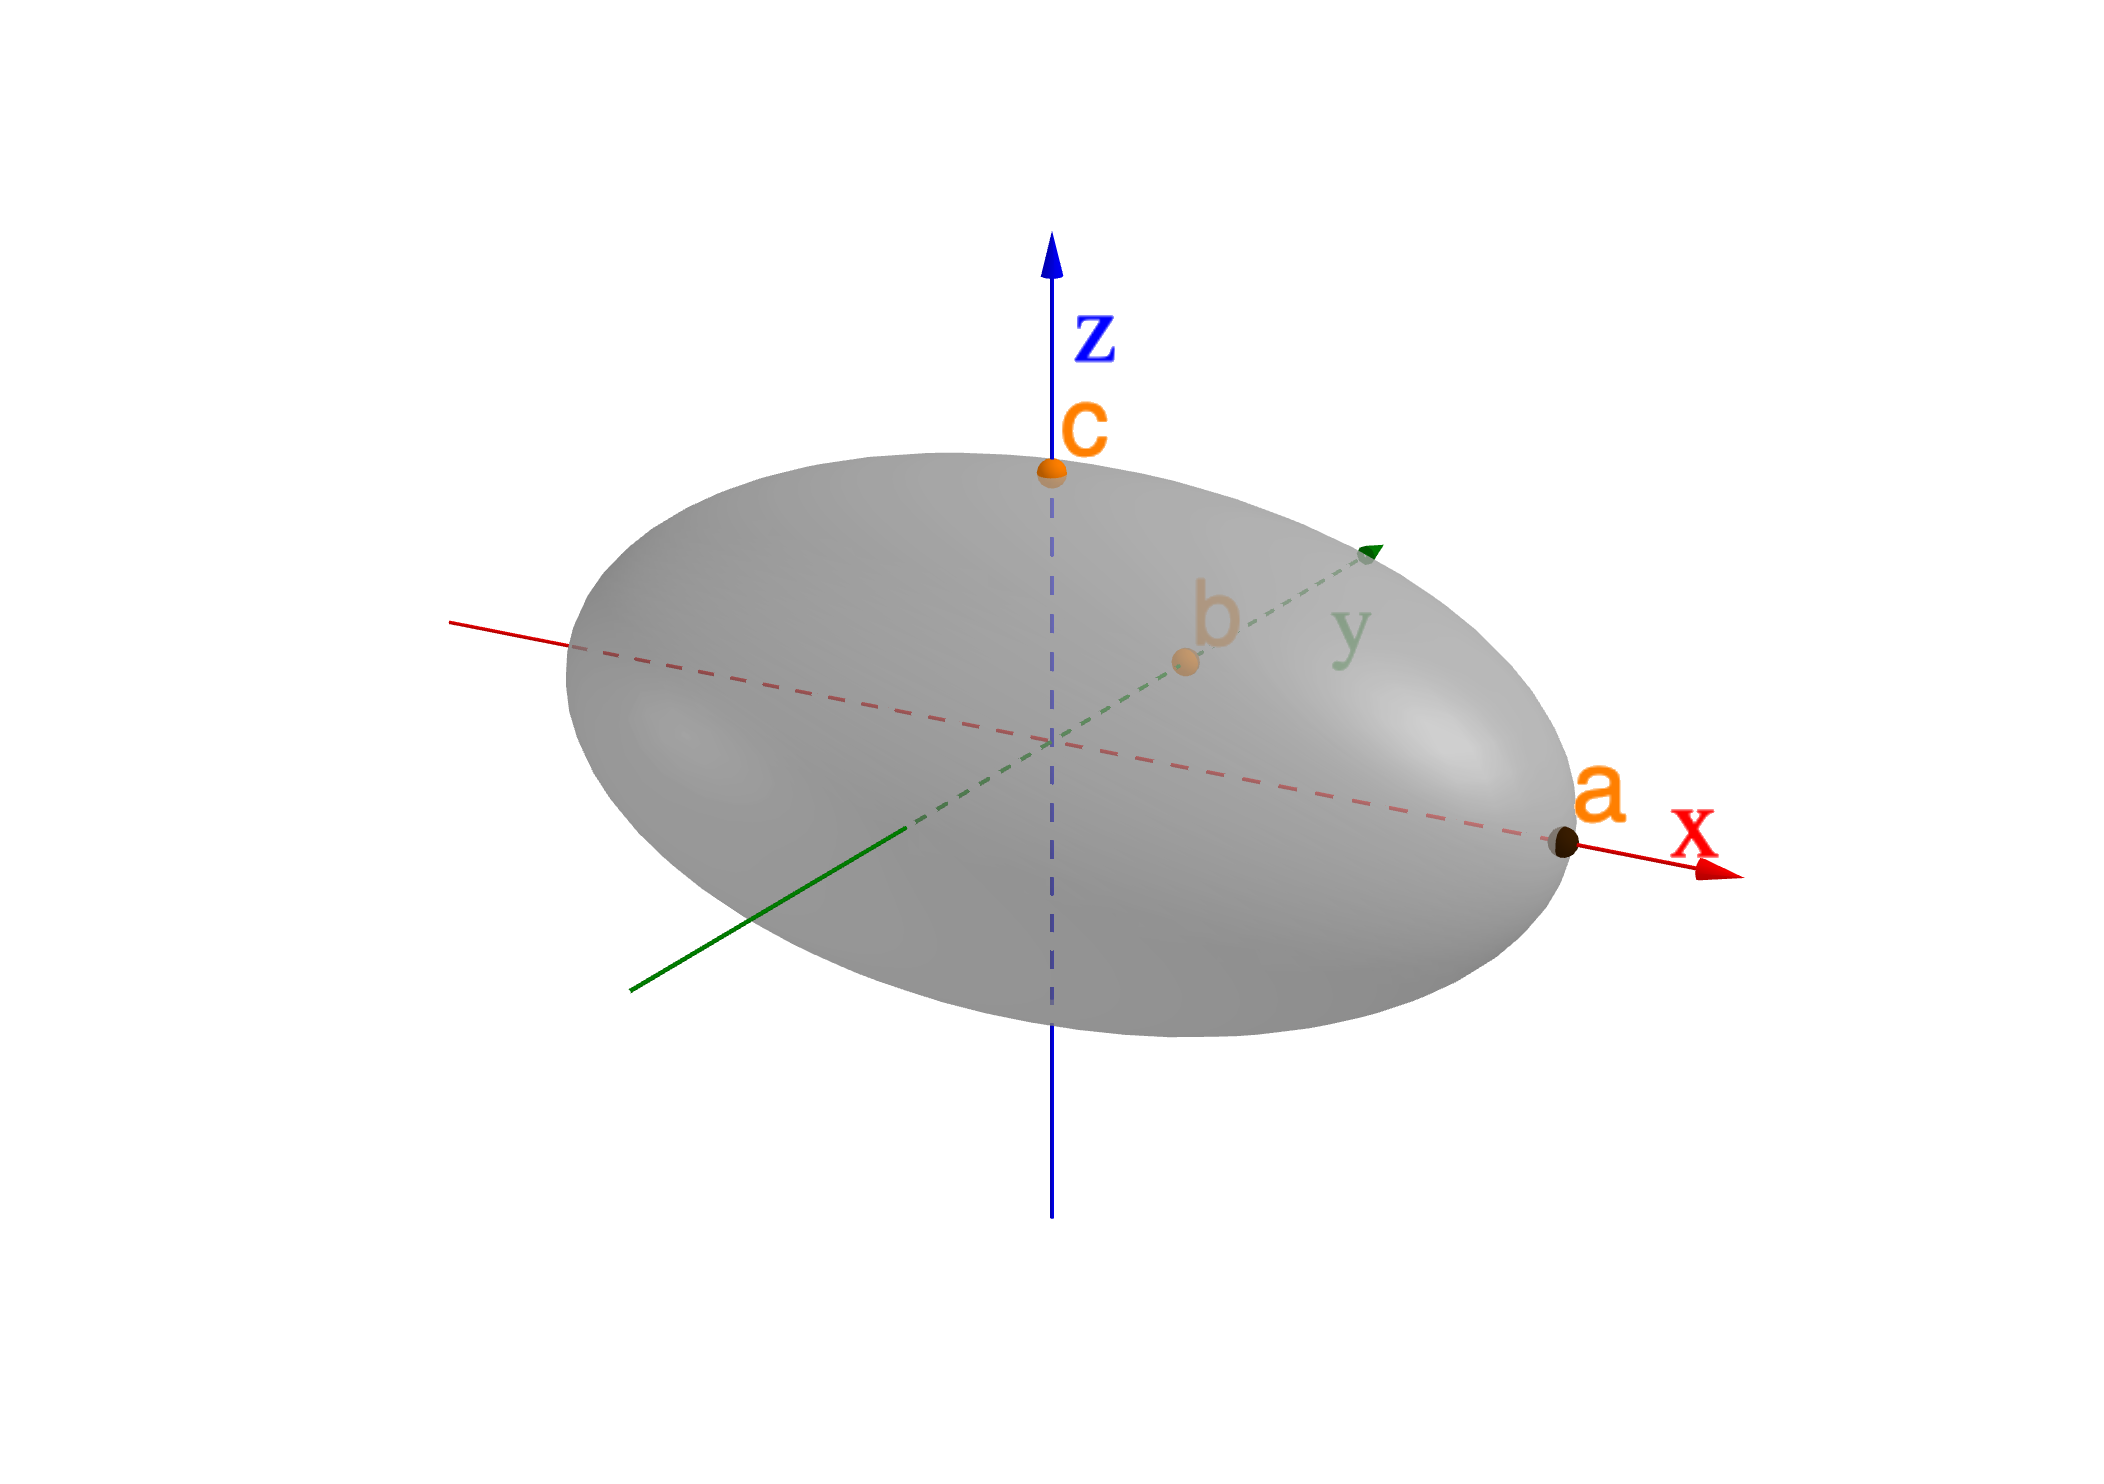
\includegraphics[width=0.5\textwidth]{Plots/ellipsoid.png} \end{center}

\subsubsection*{Surfaces Attained Through Rotation: $r^2 = x^2 + y^2$}

When the variables $x$ and $y$ appear together as $x^2 + y^2$, this signals that the surface is attained through rotation. Set a new variable $r$, with $r^2 = x^2 + y^2$. We graph the equation involving $z$ and $r$ in the $rz$-plane, with $r > 0$ only. We then revolve the curve around the $z$-axis to attain the surface in 3D: the $r$-axis stands for both $x$-axis and $y$-axis.

\begin{exercise}
    Sketch the following curves.

    \begin{minipage}[t]{0.45\linewidth} \setstretch{2.25}
        \begin{enumerate}
            \item $x = 2y^2$
            \item $\frac{x^2}{2} + \frac{y^2}{9} = 1$
            \item $x^2 + 2y^2 = 4$
        \end{enumerate}
    \end{minipage}
    \begin{minipage}[t]{0.45\linewidth} \setstretch{2.25}
        \begin{enumerate} \setcounter{enumi}{3}
            \item $x^2 + 3y^2 + 2x - 12y + 10 = 0$
            \item $y^2 - x^2 = 1$
            \item $\frac{(x - 2)^2}{4} - \frac{(y + 2)^2}{9} = 1$
        \end{enumerate}
    \end{minipage}
\end{exercise}

\begin{exercise}
    Sketch the following surfaces.

    \begin{minipage}[t]{0.45\linewidth} \setstretch{2.25}
        \begin{enumerate}
            \item $x^2 + y^2 = 1$

            \item $z = x^2 + y^2$

            \item $z^2 = x^2 + y^2$
        \end{enumerate}
    \end{minipage}
    \begin{minipage}[t]{0.45\linewidth} \setstretch{2.25}
        \begin{enumerate} \setcounter{enumi}{3}
            \item $x^2 + y^2 + \frac{z^2}{4} = 1$
            \item $z = \left( \sqrt{x^2 + y^2} - 1 \right)^2$
            \item $x^2 + y^2 + z^2 = 2z$
        \end{enumerate}
    \end{minipage}
\end{exercise}

\chapterimage{c2.png}

\chapter{Vectors and the Geometry of Space}

\section{Vector and Matrix}

A point in 2D needs 2 coordinates. It is typically written as, for example: $$\vec{a} = (1, 2) \quad\text{or}\quad \vec{a} = \begin{bmatrix} 1 \\ 2 \end{bmatrix}$$ This is the point $x = 1$ and $y = 2$ on the 2D $xy$-plane.

A point in 3D needs 3 coordinates. It is typically written as, for example: $$\vec{b} = (0, 2, 1) \quad\text{or}\quad \vec{b} = \begin{bmatrix} 0 \\ 2 \\ 1 \end{bmatrix}$$ This is the point $x = 0$, $y = 2$, and $z = 1$ in 3D space.

The point can also be interpreted as a \term{vector}\index{Vector}, written in the same way. We can also think of a vector as an \itblue{arrow} from the origin to the point.

Typically, it doesn't matter if we write the vector horizontally or vertically.

\begin{definition}[Matrix]\index{Matrix}
    A \term{matrix} is a block of numbers written in a rectangle (or square) in a specific order.
\end{definition}

For example, A is a $2 \times 3$ (2 by 3) matrix, with 2 rows and 3 columns: $$A = \begin{bmatrix} a & b & c \\ d & e & f \end{bmatrix}$$

We may think of vectors as $1 \times n$ or $n \times 1$ matrix (for $n = 2$ or $3$). We can add matrices, and multiply matrices by a scalar (number).

{~~~}

\begin{itemize}
    \item $\begin{bmatrix} a & b \\ c & d \end{bmatrix} + \begin{bmatrix} e & f \\ g & h \end{bmatrix} = \begin{bmatrix} a + e & b + f \\ c + g & d + h \end{bmatrix}$
    \item $r\begin{bmatrix} a & b \\ c & d \end{bmatrix} = \begin{bmatrix} ra & rb & rc & rd \end{bmatrix}$
\end{itemize}

{~~~}

Standard arithmetic rules apply. For matrices $A$, $B$, and scalar $c$:

\begin{itemize}
    \item $A + B = B + A$
    \item $cA = Ac$
    \item $c(A + B) = cA + cB$
\end{itemize}

\section{Determinant}\index{Determinant}

The determinant of a \bred{square} matrix is a number.

Starting at the first row, first position, write down this value, and remove this row and this column from the original matrix. Multiply this value by the determinant of the remaining matrix.

$$\det \begin{bNiceMatrix} a & b & c \\ d & e & f \\ g & h & i \CodeAfter \tikz \draw (1-1) circle (1.8mm); \end{bNiceMatrix} = a \cdot \det \begin{bmatrix} e & f \\ h & i \end{bmatrix} \dots$$

Now, move right, write down this value, and remove this row and this column from the original matrix. Multiply this value to the determinant of the remaining matrix with a \bred{minus sign}.

$$\det \begin{bNiceMatrix} a & b & c \\ d & e & f \\ g & h & i \CodeAfter \tikz \draw (1-2) circle (1.8mm); \end{bNiceMatrix} = a \cdot \det \begin{bmatrix} e & f \\ h & i \end{bmatrix} {\color{red}-}~ b \cdot \det \begin{bmatrix} d & f \\ g & i \end{bmatrix}$$

Now, move right again and repeat until we have reached the last column. The positive and negative signs need to \bred{alternate}.

$$\det \begin{bNiceMatrix} a & b & c \\ d & e & f \\ g & h & i \CodeAfter \tikz \draw (1-3) circle (1.8mm); \end{bNiceMatrix} = a \cdot \det \begin{bmatrix} e & f \\ h & i \end{bmatrix} - b \cdot \det \begin{bmatrix} d & f \\ g & i \end{bmatrix} {\color{red}+}~ c \cdot \begin{bmatrix} d & e \\ g & h \end{bmatrix}$$

Each time we apply the algorithm, we end up with several new determinants to calculate, but with matrices of \itblue{smaller sizes}.

$$\det \begin{bmatrix} a & b \\ c & d \end{bmatrix} = ad = bc$$

Determinant does not behave well with addition and scalar multiplication:
$$\det(A + B) \neq \det(A) + \det(B) \qquad \det(cA) \neq c \cdot \det(A)$$

\begin{exercise}
    Find the determinant.

    {~~~}

    \begin{enumerate}
        \item $\begin{bmatrix} 3 & -1 \\ 2 & 5 \end{bmatrix}$

        {~~~}

        \item $\begin{bmatrix} 3 & 3 & -3 \\ -3 & -5 & 2 \\ -4 & 4 & -6 \end{bmatrix}$

        {~~~}

        \item $\begin{bmatrix} 3 & 1 & 0 \\ 1 & 3 & 4 \\ 0 & 0 & 4 \end{bmatrix}$
    \end{enumerate}
\end{exercise}

\section{Dot product}

2 vectors can form a \term{dot product}\index{Dot Product}, and the result is a scalar (number).

$$\vec{x} \cdot \vec{y} = \begin{bmatrix} x_1 \\ x_2 \\ \vdots \end{bmatrix} \cdot \begin{bmatrix} y_1 \\ y_2 \\ \vdots \end{bmatrix} = x_1y_1 + x_2y_2 + \cdots$$

Note that this dot product is different from scalar multiplication, as we are multiplying 2 vectors together, not a scalar with a vector.

The \term{length} (absolute value, or \term{norm})\index{length (of a Vector)}\index{Absolute Value (of a Vector)}\index{Norm} of a vector using the Pythagoras Theorem: $$| \vec{x} | = \sqrt{\vec{x} \cdot \vec{x}} = \sqrt{(x_1)^2 + (x_2)^2 + \cdots}$$

Similarly, define the distance between two points using pythagoras Theorem: $$d(\vec{x}, \vec{y}) = | \vec{x} - \vec{y} | = \sqrt{(y_1 - x_1)^2 + (y_2 - x_2)^2 + \cdots}$$

Going from a point a to point c, is always shorter than going to some other point b first and then back to c. This is called the \term{Triangle Inequality}\index{Triangle Inequality}: $$d(\vec{a},\vec{c}) \le d(\vec{a},\vec{b}) + d(\vec{b},\vec{c})$$ $$| \vec{x} + \vec{y} | \le | \vec{x} | + | \vec{y} |$$

Let $\theta$ be the angle between $\vec{x}$ and $\vec{y}$, the dot product is also given by $$\vec{x} \cdot \vec{y} = | \vec{x} | | \vec{y} | \cos \theta$$

Thus, 2 vectors are \term{orthogonal}\index{Orthogonal} (perpendicular\index{Perpendicular}) if the dot product is zero.

The dot product have the usual properties of multiplication:

\begin{itemize}
    \item $\vec{a} \cdot \vec{b} = \vec{b} \cdot \vec{a}$
    \item $\vec{a} \cdot (\vec{b} + \vec{c}) = \vec{a} \cdot \vec{b} + \vec{a} \cdot \vec{c}$
    \item $c(\vec{a} \cdot \vec{b}) = (c\vec{a}) \cdot \vec{b} = a \cdot (c\vec{b})$
\end{itemize}

Note that since the dot product needs two vectors and produce a number, a quantity such as $\vec{a} \cdot \vec{b} \cdot \vec{c}$ is not well defined.

\begin{exercise}
    Find the length of the vectors. Find $\vec{a} \cdot \vec{b}$ and the angle between them.

    {~~~}

    \begin{enumerate}
        \item $\vec{a} = (4, 3)$, $\vec{b} = (2, -1)$
        \item $\vec{a} = (4, 0, 2)$, $\vec{b} = (2, -1, 0)$
    \end{enumerate}
\end{exercise}

\section{Cross product}

2 vectors (in 3D) can form a \term{cross product}\index{Cross Product}, and the result is a \itblue{vector} (in 3D).

Let $\vec{x} = (x_1, x_2, x_3)$, $\vec{y} = (y_1, y_2, y_3)$ in 3D.

We typically write the cross product using determinant:

$$\vec{x} \times \vec{y} = \det \begin{bmatrix} i & i & k \\ x_1 & x_2 & x_3 \\ y_1 & y_2 & y_3 \end{bmatrix}$$ $$\vec{x} \times \vec{y} = i(x_2y_3 - x_3y_2) - j(x_1y_3 - x_3y_1) + k(x_1y_2 - x_2y_1)$$ $$\vec{x} \times \vec{y} = (x_2y_3 - x_3y_2, x_1y_3 - x_3y_1, x_1y_2 - x_2y_1)$$

The notations $i = (1, 0, 0)$, $j = (0, 1, 0)$, $k = (0, 0, 1)$ are very easy to use, where the quantity attached to $i$ is the first component of the vector, and the quantity attached to $j$ would be the second, and $k$ would be the third.

The vector produced by the cross product, $\vec{x} \times \vec{y}$, would be orthogonal to both vectors $\vec{x}$ and $\vec{y}$. Notice that in most cases, there would be 2 such vectors with this property. They are exactly $$\vec{x} \times \vec{y} \qquad\text{and}\qquad -\vec{x} \times \vec{y}$$

In fact, we have $$\vec{x} \times \vec{y} = - \vec{y} \times \vec{x}$$

Notice that the order of a dot product does not matter, but the order of cross product matters up to a negative sign.

The other usual properties of multiplication hold:

\begin{itemize}
    \item $(a\vec{a} \times \vec{b}) = c(\vec{a} \times \vec{b}) = a \times (c\vec{b})$
    \item $\vec{a} \times (\vec{b} + \vec{c}) = \vec{a} \times \vec{b} + \vec{a} \times \vec{c}$
\end{itemize}

Similar to the dot product, we can also relate the angle between the 2 vectors, $$| \vec{x} \times \vec{y} | = | \vec{x} | | \vec{y} | \sin \theta$$

Note that since $\vec{x} \times \vec{y}$ is a vector, we need to take its absolute value. So 2 vectors are \itblue{parallel} if the cross product is zero.

\begin{exercise}
    Let $\vec{x} = (3, -2, 1)$, $\vec{y} = (1, -1, 1)$. Find $\vec{x} \times \vec{y}$.
\end{exercise}

\section{Lines and Planes}

For a \term{line}\index{Line} to be defined, we need a direction $\vec{v}$ and a point on the line $\vec{r}_0$. $$\begin{bmatrix} x \\ y \\ z \end{bmatrix} := \vec{r} = t\vec{v} + \vec{r}_0$$

The vector $\vec{r}$ and the value $t$ do not need to be determined \footnote{$\vec{v}$ and $\vec{r}_0$ are not unique, and any correct pair would give the right equation. }.

For a \term{plane}\index{Plane} to be defined, we need a \bred{normal vector} $\vec{n} = (a, b, c)$ and a point on the plane $\vec{r}_0$. $$\vec{n} \cdot \vec{r} = \vec{n} \cdot \vec{r}_0$$ $$ax + by + cz = \vec{n} \cdot \vec{r}_0$$ where $\vec{r}$ is the same as above and does not need to be determined. The \term{normal vector}\index{Normal Vector (of a Plane)} $\vec{n}$ is orthogonal to the plane \footnote{Similar to lines, $\vec{v}$ and $\vec{r}_0$ are not unique. }.

\subsubsection*{Plane Defined by 3 Points}

Consider 3 points $\vec{u}$, $\vec{v}$, and $\vec{w}$. We can connect any 2 pairs of points together to create 2 direction vectors which are inside the plane. For example, we may take $\vec{x} = \vec{u} - \vec{v}$, and$ \vec{y} = \vec{w} - \vec{v}$. From there we can form the cross product to attain a vector that is orthogonal to both vectors inside the plane, so the cross product would be the normal vector, which is orthogonal to the plane.

\begin{exercise}
    Find the equation of the line or plane.

    {~~~}

    \begin{enumerate}
        \item The line through $(-8, 0, 4)$ and $(3, -2, 4)$.
        \item The plane through the origin and perpendicular to the vector $(1, 5, 2)$.
        \item The plane through $(2, 4, 6)$ parallel to the plane $x + y - z = 5$.
        \item The plane through $(0, 1, 1)$, $(1, 0, 1)$, and $(1, 1, 0)$.
        \item The plane equidistant from point $(3, 1, 5)$ and $(-2, 0, 0)$.
    \end{enumerate}
\end{exercise}

\chapterimage{c3.png}

\chapter{Partial Derivatives}

\section{Multivariable Function}

In first year, we study 1D functions: \term{functions of one variable}\index{Function of One Variable}, as $f(x)$. This can be plotted in 2D plane, with $y = f(x)$. Now, we can study functions of multiple variables.

\begin{definition}[2D Function]\index{2D Function}
    A \term{2D function}, $f(x, y)$, has 2 inputs being $x$, $y$, and 1 output.
\end{definition}

Sometimes, we can label the output as $z = f(x, y)$.

We can plot this 2D function in 3D space, where the height $z$ above the point $(x, y)$ on the $xy$-plane is equal to $f(x, y)$.

This would give a graph, which is a surface.

Alternatively, $z = f(x, y)$ can be thought of as an equation which involves $x$, $y$, and $z$, which would also give a surface in 3D space.

However, similar to 1D functions, given an equation involving $x$, $y$, and $z$, it is not always possible to isolate $z$ into $z = f(x, y)$.

Examples of 2D functions include: $$f(x, y) = x^2 + 2y \qquad f(x, y) = xe^{xy} \qquad f(x, y) = \sin(xy^2)$$

\begin{definition}[3D Function]\index{3D Function}
    A \term{3D function}, $f(x, y, z)$, has 3 inputs being $x$, $y$, and $z$, and 1 output.
\end{definition}

It is possible to label the output as $w = f(x, y, z)$, but this is typically not useful as this introduces a 4th variable. The ``plot'' of this function would be in 4D space, which does not exist.

Examples of 3D functions include: $$f(x, y, z = x^2 + 2z - 1) \qquad f(x, y, z) = ye^{xz}$$

\begin{definition}[Level Set]\index{Level Set}
    The \term{level set} of $f$ at $k$ is given by setting $f$ to be equal to the constant $k$. This will reduce the dimension of $f$ by 1.
\end{definition}

\begin{exercise}
    $\text{ }$

    \begin{itemize}
        \item Draw the level set of $f(x, y) = 4x^2 + y^2 + 1$ for $k = 2$ and $k = 5$.
        \item Draw the level set of $f(x, y, z) = x^2 + y^2 - z$ for $k = 0$ and $k = 2$.
    \end{itemize}
\end{exercise}

\section{Limits and Continuity}

$f(x, y)$ is continuous at the 2D point $\vec{a}$ if $$\lim_{(x, y) \to \vec{a}} f(x, y) = f(\vec{a})$$

Every standard function we know are continuous in their domains. Any function transformations (such as $+$, $-$, $\times$, $/$, composition) of continuous functions, are also continuous (except division by $0$).

As most functions are continuous, most limits can be obtained by putting $(x, y) = \vec{a}$ in the formula of $f(x,y)$.

Different from 1D functions, computing limits in 2D is much more difficult. Most limit evaluation techniques from 1D functions does not work for 2D functions. In particular, there is no L'Hôpital's rule Rule for 2D functions.

Fortunately, since most functions are continuous except when dividing by $0$, we typically only need to focus on the point where the function is dividing by $0$ (and state the function is continuous everywhere else).

It turns out that it is much easier to show a limit does not exist.

\subsubsection{Test for limit that does not exist in $\mathbb{R}^2$}

Given $f(x, y)$, compute the limit as $(x, y)$ approaches $\vec{a} = (0, 0)$.

\begin{enumerate}
    \item Replace $y$ with a easy curve $y = g(x)$, passing through $\vec{a} = (0, 0)$, (such as $y = 0$, $y = x$, $y = x^2$), then let $x$ approach $0$ to attain a (1D) limit.
    \item Replace $x$ with a easy curve $x = h(y)$, passing through $\vec{a} = (0, 0)$, (such as $x = 0$, $x = y^2$), then let $y$ approach $0$ to attain a (1D) limit.
    \item Try with several different $g(x)$ and $h(y)$ to attain many (1D) limits.
    \item If you find 2 \bred{different} (1D) limits generated by 2 different curves, then the (2D) limit of $(x, y)$ approaches $\vec{a} = (0, 0)$ of $f(x, y)$ does not exist.
\end{enumerate}

Note that if all the 1D limits are the same, that is \bred{not} enough for you to conclude the 2D limit exists. To show the limit exists, we typically must use \itblue{Squeeze Theorem}.

Since most limit evaluation techniques does not work for 2D functions, it is a very fortunate fact that Squeeze Theorem does work for 2D functions. The formulation is almost the same as the 1D version.

\begin{theorem}[Squeeze Theorem]\index{Squeeze Theorem}
    {~~~}

    To attain $\lim_{(x, y) \to \vec{a}} f(x, y)$, we can try to find $g(x, y)$ and $h(x, y)$ such that

    \begin{enumerate}
        \item $g(x, y) \le f(x, y) \le h(x, y)$ near the point $\vec{a}$
        \item $\lim_{(x, y) \to \vec{a}} g(x, y) = L = \lim_{(x, y) \to \vec{a}} h(x,y)$
    \end{enumerate}

    Then we conclude $\lim_{(x, y) \to \vec{a}} f(x, y) = L$.
\end{theorem}

\subsubsection{Use Squeeze Theorem to show limit exist}

In practice, we typically want to show $\lim_{(x, y) \to \vec{a}} f(x, y) = 0$.

Start at $| f(x, y) |$, create a \itblue{chain of inequalities}, and simplify $| f(x, y) |$ to attain $| g(x, y) |$, which has limit $0$ as $(x, y)$ approaches $\vec{a}$: $$|f(x, y)| \le \cdots \le | g(x, y) | \to 0 \quad\text{i.e.}\quad \lim_{(x, y) \to \vec{a}} | g(x, y) | = 0$$ Then we conclude $\lim_{(x, y) \to \vec{a}} f(x, y) = 0$.

The typical strategy in constructing the above inequality is to remove positive quantities from the denominator of $f(x, y)$.

\begin{exercise}
    $$f(x, y) = \frac{x^2y}{x^4 + y^2} \quad\text{and}\quad f(0, 0) = 0$$

    Show the limit at $(x, y) = (0, 0)$ does not exist.
\end{exercise}

\begin{exercise}
    $$f(x, y) = \frac{xy}{\sqrt{x^4 + y^2}} \quad\text{and}\quad f(0, 0) = 0$$

    Show the function \textbf{continuous} at $(0, 0)$.
\end{exercise}

\begin{exercise}
    Find $\lim_{(x, y) \to (0, 0)} \frac{x^2 \sin^2{y}}{2x^4 + y^2}$
\end{exercise}

\section{Derivative}

Consider multivariable function $f(x, y)$ or $f(x, y, z)$.

Define the \term{derivative}\index{Derivative} to be:
$$\begin{aligned}[t]
    & \text{For } f(x, y)    &  & \nabla f = \left( \frac{\partial f}{\partial x}, \frac{\partial f}{\partial y} \right)                                \\
    & \text{For } f(x, y, z) &  & \nabla f = \left( \frac{\partial f}{\partial x}, \frac{\partial f}{\partial y}, \frac{\partial f}{\partial z} \right)
\end{aligned}$$
where $\nabla f$ is called \term{`del' $f$}\index{`del'}, or \term{gradient}\index{Gradient} of $f$.

We can interpret $\nabla f$ as a vector, even though $f(x, y)$ or $f(x, y, z)$ is a scalar.

The quantities in $\nabla f$ such as $\frac{\partial f}{\partial x}$ are called \term{partial derivatives}\index{Partial Derivative}. When taking partial derivatives with respect to a variable, we regard \bred{all other variables} as \itblue{constants} and take the derivative as usual. Sometimes, we use the notations $$\frac{\partial f}{\partial x} = f_x \qquad \frac{\partial f}{\partial y} = f_y \qquad \frac{\partial f}{\partial z} = f_z$$

\begin{example}
    Let $f(x, y) = x^2 y^3 + x$. 

    To take the partial derivative with respect to $x$, $\frac{\partial f}{\partial x}$, we view $y$ as constant. 
    $$\frac{\partial f}{\partial x} = 2xy^3 + 1$$

    To take the partial derivative with respect to $y$, $\frac{\partial f}{\partial y}$, we view $x$ as constant. 
    $$\frac{\partial f}{\partial y} = 3x^2y^2$$
\end{example}

\begin{example}
    Let $f(x, y, z) = x^2z + yz^2$. 

    To take the partial derivative with respect to $x$, $\frac{\partial f}{\partial x}$, we view \bred{both} $y$ and $z$ as constants. Similarly, for other partial derivatives, 
    $$\frac{\partial f}{\partial x} = 2xz \qquad \frac{\partial f}{\partial y} = z^2 \qquad \frac{\partial f}{\partial z} = x^2 + 2yz$$
\end{example}

\begin{exercise}
    Computer $\nabla f$. 

    \begin{minipage}[t]{0.45\linewidth} \setstretch{2}
        \begin{enumerate}
            \item $f(x, y) = (x^2 - 1)(y + 1)$
            \item $f(x, y) = (xy - 2)^2$
            \item $f(x, y) = \frac{2}{x + 3y}$
        \end{enumerate}
    \end{minipage}   
    \begin{minipage}[t]{0.45\linewidth} \setstretch{2}
        \begin{enumerate}
            \setcounter{enumi}{3}
            \item $f(x, y) = x^{x + 4y}$
            \item $f(x, y, z) = x^2 + 2z - 1$
            \item $f(x, y, z) = ye^{xz}$
        \end{enumerate}
    \end{minipage}   
\end{exercise}

\section{Directional Derivative}

Remember one dimensional derivatives in first year?
$$f'(a) = \lim_{h \to 0} \frac{f(a + h) - f(a)}{h}$$ where $f$ is defined on the real line.

We start at the point $x = a$, and we ask, if we move just a tiny bit away from $x = a$, how much does the function change?

We generalize this idea of moving a tiny bit away in higher dimensions. In the real line, we can move only left or right. In 2D, we can move in any direction we like (on the plane).

We can describe the direction of movement by a \term{unit vector}, similar to the direction vector of the equation of a line. The \term{directional derivative}\index{Directional Derivative} toward the direction $\vec{u}$ at the point $\vec{a}$ \footnote{This is a 1D limit, as $h$ is a number (the length of the movement). }: $$D_{\vec{u}} f(\vec{a}) = \lim_{h \to 0} \frac{f(\vec{a} + h\vec{u}) - f(\vec{a})}{h}$$ 

This is also the \term{rate of change}\index{Rate of Change} of the function in the direction $\vec{u}$ at the point $\vec{a}$. 

Given a vector $\vec{v}$, we can turn it into a \term{unit vector} $\vec{u} = \frac{\vec{v}}{| \vec{v} |}$. 

\begin{definition}[Unit Vector]\index{Unit Vector}
    A \term{unit vector} is a vector whose length (norm) is exactly $1$. 
\end{definition}

{~~~}

Some useful facts:

\begin{enumerate}
    \item Partial derivatives are directional derivatives with $\vec{u}$ being in a \term{coordinate direction}. For example, for $f(x,y)$, 

    \begin{itemize}
        \item $\frac{\partial f}{\partial x} = D_{\vec{u}} f$ with $\vec{u} = (1, 0)$;
        \item $\frac{\partial f}{\partial y} = D_{\vec{u}} f$ with $\vec{u} = (0, 1)$;
    \end{itemize}

    {~~~}

    \item If $f$ is \bred{differentiable}, then all directional derivative exist and $$D_{\vec{u}} f = \nabla f \cdot \vec{u}$$ where $\vec{u}$ is a \bred{unit vector}. 
    
    This formula gives an easy way to calculate directional derivative.

    {~~~}

    \item We can interpret $\nabla f(\vec{a})$ as a vector. 
    
    If we evaluate $\nabla f$ at a point $\vec{a}$, and if we interpret the vector $\nabla f(\vec{a})$ as a direction, then the directional derivative in the direction of $\nabla f(\vec{a})$ at the point $\vec{a}$ is the largest, and the value of this maximum directional derivative is equal to $| \nabla f(\vec{a}) |$. 

    {~~~}

    \item Recall equation of plane: $\vec{n} \cdot \vec{r} = \vec{n} \cdot \vec{r}_0$
    
    For $f(x, y, z) = k$ for some constant $k$, gives a \term{level set} surface. Define the \term{tangent plane} at some fixed point $\vec{r}_0 = (x_0, y_0, z_0)$ by the \bred{normal vector} $\vec{n} = \nabla f(x_0, y_0, z_0)$.

    {~~~}

    For example, consider $f(x,y) = x^2 + y^2$. 

    $\nabla f = (2x, 2y)$. At $(1,0)$, $\nabla f = (2,0)$. 

    \begin{center}
        \tikzsetnextfilename{c03s04-f01}%
        \begin{tikzpicture}
                \draw[->] (-3.7,0) -- (3.7,0) node[right] {$x$};
                \draw[->] (0,-2.7) -- (0,2.7) node[above] {$y$};
                
                \draw[thick,orange] (0,0) circle (1cm);
                \draw[thick,DarkGreen] (0,0) circle(2cm); 
                
                \draw[thick,pink,->] (1,0) -- (1,1) node[above] {Tangent to the level set};
                \draw[thick,blue,->] (1,0) -- (3,0) node[below] {$\nabla f$, orthogonal to the level set};
                
                \node[orange] at (-1,1) {$k=1$};
                \node[DarkGreen] at (-1.5,2) {$k=2$};
            \end{tikzpicture}
    \end{center}
\end{enumerate}

\begin{exercise}
    $f(x, y, z) = e^{2x}y + y^2 + 4$. At the point $(0, 0)$, find the directional derivative along the direction given by $\vec{u} = (1, 3)$ (first turn $\vec{v}$ into a unit vector). 
\end{exercise}

\begin{exercise}
    $f(x, y, z) = x^2y + z$. At the point $(2, 2, 1)$, find the maximum rate of change, and the direction with the maximum (the direction with maximum rate of change is $\nabla f$, and the value of this maximum rate of change is $| \nabla f |$). 
\end{exercise}

\begin{exercise}
    Define $f(x, y, z) = xy^2e^z$. Let $f(x, y, z) = e$. 

    At the point $(1, 1, 1)$, find the equation of the tangent plane.
\end{exercise}

\begin{exercise}
    Find all directional derivatives at $(0, 0)$ (including the partials), if they exist. Is the function \textbf{continuous} at $(0, 0)$?
    \begin{enumerate}[label=\alph*)]
        \item 
        $f(x, y) = \begin{cases}
            \frac{xy}{x^2 + y^2} & (x, y) \neq (0, 0) \\
            0                    & (x, y) = (0, 0)
        \end{cases}$

        \item $f(x, y) = \sqrt{|xy|}$
    \end{enumerate}

    {~~~}

    \textbf{Strategy:}

    When the function has division by $0$, or some other problems at the origin (such as absolute value or square root), we must use the definition of directional derivative, because $f$ \bred{may not be differentiable} at $(0, 0)$ so the formula $\nabla f \cdot \vec{u}$ does not work. Set $\vec{a} = (0, 0)$ and $\vec{u} = (a, b)$ where $a^2 + b^2 = 1$. 
\end{exercise}

\section{Differentiation}

In first year, we defined the tangent line to be $\frac{\text{rise}}{\text{run}}$, and we calculate the limit as the \textit{run} approaches $0$, where the {\color{DarkGreen}secant line} becomes the {\color{orange}tangent line}. This gives the slope of the tangent line of the function at $x = a$.

\begin{center}
    \tikzsetnextfilename{c03s05-f01}%
    \begin{tikzpicture}
        \draw[->] (-2.7,0) -- (2.7,0) node[right] {$x$};
        \draw[->] (-1.5,-0.7) -- (-1.5,3.2) node[above] {$y$};

        \draw[thick,blue,domain=-2.2:2.7] plot (\x, {(\x/3)^2+(\x/2)+1});

        \draw[thick,orange,domain=-2.2:2.7] plot (\x, {\x/2+1});
        \draw[thick,DarkGreen,domain=-2.2:2.7] plot (\x, {3*\x/4+1});

        \draw[orange,fill=orange] (0,1) circle (0.075cm);
        \draw[DarkGreen,fill=DarkGreen] (0,1) circle (0.045cm);
        \draw[DarkGreen,fill=DarkGreen] (2.25,2.6875) circle (0.045cm);

        \draw[red,dashed] (0,1) -- (0,0) node[below] {$a$};
        \draw[DarkGreen,dashed] (2.25,2.6875) -- (2.25,0) node[below] {$a+h$};
        \draw[red,dashed] (0,1) -- (-1.5,1) node[left] {$f(a)$};
        \draw[DarkGreen,dashed] (2.25,2.6875) -- (-1.5,2.6875) node[left] {$f(a+h)$};

        \node[blue] at (-2.25,0.125) {$f(x)$};
    \end{tikzpicture}
\end{center}

There is another way to interpret the tangent line, however. It is the \itblue{best approximation of the function} using a line. Let $L(x)$ be the equation of the tangent line, and $g(x)$ be the equation of a random line that passes through $(a, f(a))$. Why is $\color{orange} L(x)$ the tangent line and not $\color{DarkGreen}g(x)$?

\begin{center}
    \tikzsetnextfilename{c03s05-f02}%
    \begin{tikzpicture}
        \draw[->] (-2.7,0) -- (2.7,0) node[right] {$x$};
        \draw[->] (-1.5,-0.7) -- (-1.5,3.2) node[above] {$y$};

        \draw[thick,blue,domain=-2.2:2.7] plot (\x, {(\x/3)^2+(\x/2)+1});

        \draw[thick,orange,domain=-2.2:2.7] plot (\x, {\x/2+1});
        \draw[thick,DarkGreen,domain=-1:1.25] plot (\x, {2*\x+1});

        \draw[red,dashed] (0,1) -- (-0,0) node[below] {$a$};

        \draw[red,fill=red] (0,1) circle (0.05cm) node[above left] {$(a, f(a))$};

        \node[blue] at (-2.25,0.125) {$f(x)$};
        \node[orange] at (2,1.5) {$L(x)$};
        \node[DarkGreen] at (-0.25,-0.75) {$g(x)$};
    \end{tikzpicture}
\end{center}

Clearly, the error made from $L(x)$, $f(x) - L(x)$ goes to $0$ as $x \to a$. However, $\lim_{x\to{a}}g(x)$ is also $0$. It is not sufficient to say that the error goes to $0$, but we also want to check the rate at which the error goes to $0$. So what makes $\color{orange}L(x)$ better than $\color{DarkGreen}g(x)$? While both are approaching $0$, the error for $\color{orange} L(x)$ approaches $0$ \bred{faster} than that of $\color{DarkGreen} g(x)$ \footnote{To denote ``$F(x)$ goes to $0$ faster than $G(x)$'', we use $\lim_{x\to0} \frac{F(x)}{G(x)} = 0$. }. For the tangent line, we want $L(x)$ to approach $f(a)$ the fastest, in particular, faster than how $x$ approached $a$. Thus, we have $\lim_{x\to{a}} \frac{f(x) - L(x)}{x} = 0$.

Recall that the equation of the tangent line is $y - f(a) = f'(a)(x - a)$, so $L(x) = f(a) + f'(a)(x - a)$ \footnote{This is in fact the first order Taylor expansion of $f(x)$ at $a$. }, where $f'(a) = \lim_{h\to0} \frac{f(a+h) - f(a)}{h}$ as before. Take $x = a + h$, we have alternatively
\begin{align*}
    \lim_{h\to0} \frac{f(a + h) - L(a + h)}{h - a}                                       & = 0     \\
    \lim_{h\to0} \frac{f(a + h) - \left[ f(a) + f'(a)(\cancelto{h}{x - a})~~ \right]}{a} & = 0     \\
    \lim_{h\to0} \frac{f(a + h) - f(a)}{h} - \frac{f'(a) \cdot \cancel{h}}{\cancel{h}}   & = 0     \\
    \lim_{h\to0} \frac{f(a + h) - f(a)}{h}                                               & = f'(a)
\end{align*}

This happens to be the equation we have before.

    {~~~}

We can expand this result to higher dimensions. If we have a 2D function, we should have a \term{tangent plane} that allows the error between the function and the tangent plane to approach $0$ faster than any other planes.

Given the tangent plane $w = L(x,y)$, we want $\lim_{\vec{x}\to\vec{a}} f(x,y) - L(x,y) = 0$, and approaches $0$ the fastest. That is, $\lim_{\vec{x}\to\vec{a}} \frac{f(x,y) - L(x,y)}{| \vec{x} - \vec{a} |} = 0$ \footnote{Similar as before, this means we want the error to approach $0$ faster than $\vec{x}$ approaches $\vec{a}$. }.

To get the equation of the tangent plane, we can think of the original function, $f(x,y)$, as the level set of the 3D function $F(x,y,z) = f(x,y) - z$ at $k = 0$. Then, by the result from the previous section, $\nabla F(x_0,y_0,z_0)$ is the normal vector to the tangent plane at the given point $(x_0,y_0,z_0)$. That is, $\vec{n} = \nabla F = \left( \frac{\partial F}{\partial x}, \frac{\partial F}{\partial y}, \frac{\partial F}{\partial z} \right) = \left( \frac{\partial f}{\partial x}, \frac{\partial f}{\partial y}, -1 \right)$.

Note that at $\vec{a} = (x_0, y_0)$, we obtain the point $(x_0, y_0, f(\vec{a}))$ on the graph of $f(x,y)$. Denote this point $\vec{r}_0$, and this allows us to get the formula for the tangent plane.
\begin{align*}
    \vec{n} \cdot \vec{r}
     & = \vec{n} \cdot \vec{r}_0 \\
    \left( \frac{\partial f}{\partial x}, \frac{\partial f}{\partial y}, -1 \right) \cdot \vec{r}
     & = \left( \frac{\partial f}{\partial x}, \frac{\partial f}{\partial y}, -1 \right) \cdot \left( x_0, y_0, f(\vec{a}) \right) \\
    \frac{\partial f}{\partial x} \cdot x + \frac{\partial f}{\partial y} \cdot y - z
     & = \frac{\partial f}{\partial x} \cdot x_0 + \frac{\partial f}{\partial y} \cdot y_0 - f(\vec{a}) \\
    z
     & = f(\vec{a}) + \frac{\partial f}{\partial x} (x - x_0) + \frac{\partial f}{\partial y} (y - y_0) \\
    z
     & = f(\vec{a}) + \nabla f(\vec{a}) \cdot (x-x_0, y-y_0)
\end{align*}

To further simplify this equation, take $(x,y) = \vec{x} = \vec{a} + \vec{h}$. Then, $\vec{h} = \vec{x} - \vec{a} = (x - x_0, y - y_0)$. Now, $z = f(\vec{a}) + \nabla f(\vec{a}) \cdot \vec{h}$.

Substitute the equation for $L(x,y)$ back into $\lim_{\vec{x}\to\vec{a}} \frac{f(x,y) - L(x,y)}{| \vec{x} - \vec{a} |} = 0$, we obtain
\begin{align*}
    \lim_{\vec{x}\to\vec{a}} \frac{f(x,y) - L(x,y)}{| \vec{x} - \vec{a} |}
     & = 0 \\
    \lim_{\vec{h}\to\vec{0}} \frac{f(\vec{a} + \vec{h}) - \left( f(\vec{a}) + \nabla f(\vec{a}) \cdot \vec{h} \right)}{| \vec{h} |}
     & = 0 \\
    \lim_{\vec{h}\to\vec{0}} \frac{f(\vec{a} + \vec{h}) - f(\vec{a}) - \nabla f(\vec{a}) \cdot \vec{h}}{| \vec{h} |}
     & = 0
\end{align*}

\begin{definition}[Differentiable]\index{Differentiable}
    $f$ is \term{differentiable} if the gradient vector $\nabla f(\vec{a})$ satisfies $$\lim_{\vec{h} \to \vec{0}} = \frac{f(\vec{a} + \vec{h}) - f(\vec{a}) - \nabla f(\vec{a}) \cdot \vec{h}}{| \vec{h} |} = 0$$
\end{definition}

Note that this is a \itblue{2D limit}. This limit is typically used when $\vec{a} = (0, 0)$, so we may set $\vec{h} = (x, y)$ and show the limit is zero using Squeeze Theorem.

{~~~}

Some useful facts:

\begin{enumerate}
    \item If $f$ is $C^1$ at $\vec{a}$ \footnote{This means all partial derivatives exist near $\vec{a}$ and at $\vec{a}$, and the partial derivatives are \bred{continuous} (as functions) at $\vec{a}$. }, then $f$ is differentiable at $\vec{a}$ ($\nabla f$ exists). 

    \item Being differentiable is a stronger condition than having directional derivative. If $f$ is differentiable, then all directional derivative is given by $D_{\vec{u}} f = \nabla f \cdot \vec{u}$. 

    \item If a function $f$ is differentiable at $\vec{a}$, then $f$ is continuous at $\vec{a}$.
\end{enumerate}

{~~~}

\begin{exercise}
    Define $$f(x, y) = \begin{cases}
        \frac{xy}{x^2 + y^2} & (x, y) \neq (0, 0) \\
        0                    & (x, y) = (0, 0)
    \end{cases}$$

    Show the directional derivatives exist at $(0, 0)$, but $f$ is \textbf{not differentiable} at $(0, 0)$.

    {~~~}

    \textbf{Strategy:}
    
    There are 2 ways to approach the problem.

    \begin{enumerate}
        \item If the function is \textbf{not continuous} at $(0, 0)$, then it is \textbf{not differentiable} at $(0, 0)$. So we may try to show it is not continuous at $(0, 0)$. However, some functions \textbf{are continuous} at $(0, 0)$, so we can attain no conclusion in such cases.

        \item Compute all the directional derivatives. If $f$ is differentiable, then every directional derivative should satisfy $D_{\vec{u}} f = \nabla f \cdot \vec{u}$. 
        
        Check this equation for $\vec{u} = (1, 0)$, $\vec{u} = (0, 1)$, and $\vec{u} = \left( \frac{1}{\sqrt{2}}, \frac{1}{\sqrt{2}} \right)$ (easy unit vectors). 
    \end{enumerate}
\end{exercise}

\begin{exercise}
    Show whether the function is differentiable at $(0, 0)$.

    \begin{enumerate}[label=\alph*)]
        \item $f(x, y) = \begin{cases}
            \frac{x|y|}{\sqrt{x^2 + y^2}} & (x, y) \neq (0, 0) \\
            0                             & (x, y) = (0, 0)
        \end{cases}$

        \item $f(x, y) = \begin{cases}
            \frac{x^4 + y^4}{x^2 + y^2} & (x, y) \neq (0, 0) \\
            0                           & (x, y) = (0, 0)
        \end{cases}$
    \end{enumerate}
\end{exercise}

\section{Higher Order Derivative}

We may take (partial) derivatives on top of partial derivatives. 

In 2 dimensions, for $f(x, y)$, there are 4 ways of taking second derivatives. We put them into the \term{Hessian Matrix}\index{Hessian Matrix}: 
$$H = \begin{bmatrix}
    \frac{\partial^2 f}{\partial x^2} & \frac{\partial^2 f}{\partial xy}  \\
    \frac{\partial^2 f}{\partial yx}  & \frac{\partial^2 f}{\partial y^2}
\end{bmatrix} = \begin{bmatrix}
    \frac{\partial f}{\partial x}\left( \frac{\partial f}{\partial x} \right) & 
    \frac{\partial f}{\partial x}\left( \frac{\partial f}{\partial y} \right)   \\
    \frac{\partial f}{\partial y}\left( \frac{\partial f}{\partial x} \right) & 
    \frac{\partial f}{\partial y}\left( \frac{\partial f}{\partial y} \right)
\end{bmatrix} = \begin{bmatrix}
    f_{xx} & f_{xy} \\ f_{yx} & f_{yy}
\end{bmatrix}$$

{~~~}

If $f$ is $C^2$ at $\vec{a}$ \footnote{This means all the 2nd order partial derivatives exist near $\vec{a}$ and at $\vec{a}$, and the 2nd order partial derivatives are continuous (as functions) at $\vec{a}$ (In practice, a function can fail to be continuous when there is division by zero). }, then \bred{mixed partial derivatives commute}:

The order of taking derivatives does not change the final answer: $f_{xy} = f_{yx} \to$ Taking derivative in $x$ then $y$ is the same as taking in $y$ then $x$.

In other words, if $f$ is $C^2$, then \bred{the Hessian Matrix is symmetric}.

{~~~}

We can also construct the Hessian for $f(x, y, z)$, which will be a $3 \times 3$ matrix. We can also construct higher order derivatives, such as 3rd order $f_{xyz}$ or $f_{xyy}$. In general, if $f$ is $C^k$, then mixed partial derivatives commute (up to order $k$).

\begin{exercise}
    Find the Hessian Matrix.

    \begin{minipage}[t]{0.45\linewidth} \setstretch{1.5}
        \begin{enumerate}
            \item $f(x, y) = 3x^2 + 4xy + 5y^2$
            \item $f(x, y) = \cos(x + 2y)$
            \item $f(x, y) = x^{2x + y}$
        \end{enumerate}
    \end{minipage}
    \begin{minipage}[t]{0.45\linewidth} \setstretch{1.5}
        \begin{enumerate} \setcounter{enumi}{3}
            \item $f(x, y) = e^{x^2 + y}$
            \item $f(x, y) = e^x \sin(y)$
            \item $f(x, y, z) = x^2y + xz + z^2$
        \end{enumerate}
    \end{minipage}
\end{exercise}

\begin{exercise}
    $$f(x, y) = \begin{cases}
        \frac{x^3y - xy^3}{x^2 + y^2} & (x, y) \neq (0, 0) \\
        0                             & (x, y) = (0, 0)
    \end{cases}$$

    Find $f_x$ and $f_y$ at $(x, y) = (0, 0)$ \textbf{and} $(x, y) \neq (0, 0)$. Then show $f_{xy} \neq f_{yx}$ at $(0, 0)$. i.e. Taking 2nd derivatives in different orders give different answers. 

    Is $f$ $C^2$ at $(0, 0)$ (and have we reacher a contradiction)?
\end{exercise}

\section{Critical Points}

In first year, we found critical points of functions by setting the derivative to zero. Then we check their second derivative to conclude whether critical points are max or min. In higher dimensions, it is very similar.

Let $f(x, y)$ be a 2D function (which is $C^2$).

We set $\nabla f(\vec{x}) = \vec{0}$. Solve $\vec{x}$, these are the \term{critical points}\index{Crtitial Point}.

Then we check second derivatives: \bred{the Hessian Matrix}.
$$H = \begin{bmatrix}
    \frac{\partial^2 f}{\partial x^2} & \frac{\partial^2 f}{\partial xy}  \\
    \frac{\partial^2 f}{\partial yx}  & \frac{\partial^2 f}{\partial y^2}
\end{bmatrix}$$

Note that $H$ can contain $x$ and $y$, so $H$ would be different for different points. For each critical point $\vec{a}$, 
\begin{itemize}
    \item if $\det(H(\vec{a})) > 0$, look at the top left entry
    
    \begin{itemize}
        \item if $\frac{\partial^2 f}{\partial x^2}(\vec{a}) > 0$,  then it is a \term{local minimum}\index{Local Minimum}.
        \item if $\frac{\partial^2 f}{\partial x^2}(\vec{a}) < 0$,  then it is a \term{local maximum}\index{Local Maximum}.
    \end{itemize}

    \item if $\det(H(\vec{a})) < 0$, it is a \term{saddle point}\index{Saddle Point}. 

    \item if $\det(H(\vec{a})) = 0$, it is inconclusive. 
\end{itemize}

To find the (absolute) maximum and minimum of $f$ in a region $D$, 
\begin{enumerate}
    \item Find all local extrema inside $D$ using critical points
    \item Find all extrema on the \bred{boundary} of $D$ 
    \item Compare all the function values to attain the absolute extrema
\end{enumerate}

\begin{exercise}
    Find and classify all critical points.

    \begin{enumerate}
        \item $f(x,y) = 3x^2 + 2xy + 5y^2$
        \item $f(x,y) = x^2 + 3y^4 + 4y^3 - 12y^2$
        \item $f(x,y) = (x - 1)(x^2 + y^2)$
        \item $f(x,y) = (x^2 + 2y^2)e^{-x^2 - y^2}$
    \end{enumerate}
\end{exercise}

\begin{exercise}
    Let $f(x,y) = x^2 + y^2 - 4x$

    Find the max and min indide the triangle $D$ defined by $(0, -3)$, $(0, 3)$, and $(3, 0)$. 
\end{exercise}

\section{Lagrange Multiplier}

Sometimes, we want to maximim/minimize a function on some specific curve, or there are some constraints on the variables that the function takes in. 

\begin{itemize}
    \item Take the function we want to maximize/minimize to be $f$.

    \item Take the equation that describes the constraint to be $g = 0$ (perhaps we have more than 1 constraint, so the second constraint is $h = 0$).

    \item The \term{Lagrange Multiplier Formula}\index{Lagrange Multiplier Formula} is $$\nabla f = \lambda \nabla g(+\mu \nabla h + \cdots)$$
\end{itemize}

Each constraint will create an extra $\nabla$ term on the right side with some constant in front (we need every $\nabla$ term on the right to be non-zero). 

$\lambda$ and $\mu$ are constants that you need to solve for, along with $n$ variables of $f$. The equation is an equation for vectors, so each of the components are equal. So, there are $n$ equations in the formula since $\nabla f$ has $n$ components. For each constant like $\lambda$ or $\mu$, there is a equation of constraint for each. So if there are 2 constraints, there are $n + 2$ variables that you need to solve, and you have $n + 2$ equations to do it.

You are \bred{not allowed to divide by zero} when you cancel terms. When attempting to divide a quantity $x$, you need to split into 2 cases:
\begin{itemize}
    \item When $x \neq 0$, you can divide
    \item when $x = 0$, you cannot
\end{itemize}

\begin{exercise}
    Find the max and min of the function $f(x, y)$ subject to constraints given.

    $f(x,y) = 2x - 6y$ with constraint $4x^2 + 2y^2 = 25$. 
\end{exercise}

\begin{exercise}
    Consider the curve in $\mathbb{R}^2$, $C: y = x^2$. 

    Find the point $p$ on $C$ so that the distance between $p$ and $(0, -1)$ is smallest.

    \textbf{Strategy}: We minimize $f(x, y) = \text{distance}^2 = (x - 0)^2 + (y -(-1))^2$.
\end{exercise}

\begin{exercise}
    Consider 2 curves in $\mathbb{R}^2$, $C_1: y = x^2$ and $C_2: y = x - 1$

    Find points $p$ on $C_1$ and $q$ on $C_2$ so that the distance between them is smallest.
\end{exercise}

\section{Chain Rule in 1D}

We typically think of chain rule as a rule for computation: $$f(g(x))' = f'(g(x)) \cdot g'(x)$$ where we are given a function inside another function such as $y = \sin(e^x)$, and we take the derivative of the outside (not touching the inside), then multiply the derivative of the inside.

Alternatively, we can define a \bred{variable dependence}. For example, define the variables as $y = y(t)$, and $t = t(x)$. (In the above example, we would set $y = \sin t$ and $t = e^x$.) Then we may express the chain rule (in 1D) as: $$\frac{dy}{dx} = \frac{dy}{dt} \frac{dt}{dx}$$

Intuitively, $\frac{dy}{dx}$ asks how much would $y$ change, if there is a small change in $x$. Given the variable dependence above, a small change in $x$ would cause a small change in $t$, which in turn would cause a small change in $y$. Hence, we have the 2 ``fractions'' ($\frac{dy}{dt}$ and $\frac{dt}{dx}$) on the right.

\subsection*{2nd Derivative}

We may use the above form of the chain rule to calculate the 2nd derivative.

We apply another differential operator $\frac{d}{dx}$ on top of $\frac{dy}{dx}$: $$\frac{d^2y}{dx^2} = \frac{d}{dx} \left( \frac{dy}{dx} \right)$$ Plug in the above form of the chain rule, $$= \frac{d}{dy} \left( \frac{dy}{dt} \frac{dt}{dx} \right)$$ We want to take the derivative of this product, so we need \term{product rule}\index{Product Rule (in 1D)}, $$= \frac{d}{dx}\left( \frac{dy}{dt} \right) \cdot \frac{dt}{dx} + \frac{dy}{dt} \cdot \frac{d}{dx} \left( \frac{dt}{dx} \right)$$ Notice that there are 2 types of derivatives here.

{~~~}

The 2nd term involves the expression $\frac{d}{dx} \left( \frac{dt}{dy} \right)$. Recall that we assumed $t = t(x)$ (such as $t = e^x$), so $\frac{dt}{dx}$ is also \bred{a function of $x$}. We want to take the derivative of such function \bred{against $x$}. This results in the 2nd derivative of $t = t(x)$ against $x$: $$\frac{d}{dx} \left( \frac{dt}{dx} \right) = \frac{d^2t}{dx^2}$$ The 1st term involves the expression $$\frac{d}{dx} \left( \frac{dy}{dt} \right)$$ This term is more difficult (and requires an \bred{additional expansion}). 

Recall that we assumed y = y(t) (such as y = sin t), so $\frac{dy}{dt}$ is also \bred{a function of $t$} (such as $dy = \cos t$). 

We want to take the derivative of such function \bred{against $x$}, on an expression involving $t$.

{~~~}

Notice that $\frac{dy}{dt}$ is an expression involving t, similar to $y = y(t)$. So to take the derivative against $x$, on an expression involving $t$, we know that for $y = y(t)$: $$\frac{d}{dx} \left( y(t) \right) = \frac{dy}{dx} = \frac{dy}{dt} \frac{dt}{dx} = \frac{d}{dx} \left( y(t) \right) \frac{dt}{dx}$$ Since $\frac{dy}{dt}$ is also an expression involving t, it would \bred{behave in the same way} as $y(t)$ when taking derivative \bred{against $x$}.

We can substitute $y(t)$ with $\frac{dy}{dx}$ in the above expression: $$\frac{d}{dx} \left( \frac{dy}{dt} \right) = \frac{d^2y}{dt^2}$$ 

In conclusion, to take \bred{the 2nd derivative involving chain rule}: $$\frac{d^2y}{dx^2} = \frac{d}{dx} \left( \frac{dy}{dx} \right) = \frac{d}{dx} \left( \frac{dy}{dt} \frac{dt}{dx} \right) = \frac{d}{dx} \left( \frac{dy}{dt} \right) \cdot \frac{dt}{dx} + \frac{dy}{dt} \cdot \frac{d}{dx} \left( \frac{dt}{dx} \right)$$ Taking an \bred{additional expansion} in the first term: 
$$\begin{aligned}[t]
    & = \frac{d}{dt} \left( \frac{dy}{dt} \right) \frac{dt}{dx} \cdot \frac{dt}{dx} + \frac{dy}{dt} \cdot \frac{d^2t}{dx^2} \\ 
    & = \frac{d^2y}{dt^2} \frac{dt}{dx} \cdot \frac{dt}{dx} + \frac{dy}{dt} \cdot \frac{d^2t}{dx^2}
\end{aligned}$$

Notice that we get a square of $\frac{dt}{dx}$ in the first term. Thus \bred{the chain rule formula for 2nd derivative} is: $$\frac{d^2y}{dx^2} = \frac{d^2y}{dt^2} \left( \frac{dt}{dx} \right)^2 + \frac{dy}{dt} \cdot \frac{d^2t}{dx^2} \footnote{Note $\left( \frac{dt}{dx} \right)^2 \neq \frac{d^2t}{dx^2}$. }$$ 

Of course, given a function $y = y(x)$, one would not go through this long and complicated process just to take 2nd derivative. It is much easier to just take the derivative (twice) using the computation rules.

However, this formula shines when \bred{at least one of the function is unknown}. This is exactly the case for \bred{ODE}, where $y = y(x)$ is unknown. We may use this formula to carry out a \bred{change of variables} and turn a complicated ODE into a simple one.

\subsection*{ODE - Euler Equation}

Consider $y = y(x)$. For numbers $a$, $b$, $c$, $$ax^2y'' + bxy' + cy = 0$$ This is a \term{2nd order linear equation}\index{2nd Order Linear Equation}, but with non-constant coefficients. In general, this type of equation has no solution. But here, notice that we have exactly $x^2$ in front of $y''$, and $x$ in front of $y'$.

Due to this, we can guess the solution to be $y(x) = x^n$. We plug in $y(x) = x^n$ into the ODE, and solve for $n$.

{~~~}

Typically, there will be 2 solutions for $n$. The general solution will be a linear combination of the 2 solutions (with constants $c1$ ,$c2$ in front).

\begin{example}
    $$x^2y'' - xy' - 3y = 0$$

    Take $y = x^n$, then $y' = nx^{n-1}$ and $y'' = n(n - 1)x^{n-2}$.

    Plugging into the ODE, $$x^2 n(n - 1) x^{n-2} - x n x^{n-1} - 3x^n = 0$$

    Notice that we can divide both sides by $x^n$.
    $$\begin{aligned}[t]
        n(n - 1) - n - 3 & = 0 \\
        n^2 - 2n - 3     & = 0
    \end{aligned}$$ 

    We will always get a quadratic of this form. In this case, we get $$(n - 3)(n + 1) = 0$$

    Thus the general solution is given by $$y(x) = c_1x^3 +c_2^{-1}$$
\end{example}

However, notice that given an equation with different numbers, the quadratic we get may have only one (repeated) solution. In this case, we would be ``missing'' the second solution. We can instead find the solution by using the chain rule formula for 2nd derivative. 

\begin{example}
    $$x^2y'' - 3xy' + 4y = 0$$

    If we proceed using the previous approach, we would get $(n - 2)^2 = 0$, giving one (repeated) solution.

    Instead, we can perform a change of variable, $t = \ln x$. We get 

    \begin{minipage}[t]{0.45\linewidth}
        \begin{align*}
            y' = \frac{dy}{dx} & = \frac{dy}{dt} \frac{dt}{dx} \\
                               & = \frac{dy}{dt} \frac{1}{x}
        \end{align*}
    \end{minipage}
    \begin{minipage}[t]{0.45\linewidth}
        \begin{align*}
            y'' & = \frac{d^2y}{dt^2} \left( \frac{dt}{dx} \right)^2 + \frac{dy}{dt} \cdot \frac{d^2t}{dx^2} \\
                & = \frac{d^2y}{dt^2} \left( \frac{1}{x} \right)^2 + \frac{dy}{dt} \cdot \frac{-1}{x^2}
        \end{align*}
    \end{minipage}

    Plugging the above into the ODE,
    $$\begin{aligned}[t]
        x^2y'' - 3xy' + 4y & = 0 \\
        x^2 \left( \frac{d^2y}{dt^2} \left( \frac{1}{x} \right)^2 + \frac{dy}{dt} \cdot \frac{-1}{x^2} \right) - 3x \left( \frac{dy}{dt} \frac{1}{x} \right) + 4y &= 0
    \end{aligned}$$

    Notice that all the $x$ cancels out.
    $$\begin{aligned}[t]
        \frac{d^2y}{dt^2} - \frac{dy}{dt} - 3\frac{dy}{dt} + 4y & = 0 \\
        \frac{d^2y}{dt^2} - 4\frac{dy}{dt} + 4y                 & = 0
    \end{aligned}$$

    This is a \itblue{2nd order linear equation with constant coefficients}. The solution is given by $y(t) = e^{rt}$.

    Plugging into the equation, 
    $$\begin{aligned}[t]
        r^2 - 4r + 4 & = 0 \\ 
        (r - 2)^2    & = 0
    \end{aligned}$$

    This is a \bred{repeated} root solution. Thus the general solution for $y(t)$ is given by $$y(t) = c_1 e^{2t} + c_2 t e^{2t}$$

    Since $t = \ln{x}$, we get the general solution for $y(x)$ is given by 
    $$\begin{aligned}[t]
        y(t) & = c_1 e^{2 \ln{x}} + c_2 \ln{x} e^{2 \ln{x}}                               \\
             & = c_1 \left( e^{\ln{x}} \right)^2 + c_2 \ln{x} \left( e^{\ln{x}} \right)^2 \\
             & = c_1 x^2 + c_2 (\ln{x}) x^2
    \end{aligned}$$
\end{example}

In other words, the ``missing'' second solution from the repeated root of $n = 2$, is attained by multiplying an extra factor of $\ln{x}$ in front of $x^n$.

\begin{exercise}
    Find the general solution to the ODE, where $y = y(x)$.

    {~~~}

    \begin{enumerate}
        \item $x^2y'' - 3xy' + 4y = 0$
        \item $2x^2y'' - 5xy' + 5y = 0$
        \item $x(1 - x^2)^2y'' - (1 - x^2)(1 + 4x^2)y' + 2x^3y = 0$ with the change of variable $t = \frac{-1}{2} \ln(1 - x^2)$
    \end{enumerate}
\end{exercise}

\section{Chain Rule in 2D and 3D}

Consider an example: $\begin{cases}z = z(x, y) \\ x = x(s, t) \\ y = y(s, t) \end{cases}$. We can construct the tree diagram of variable dependence.

\begin{center}
    \tikzsetnextfilename{c03s10-f01}%
    \begin{tikzpicture}[
        level 1/.style = {sibling distance = 2.5cm},
        level 2/.style = {sibling distance = 1.5cm}
    ]
    
    \node {$z$} 
        child {
            node {$x$}
            child {
                node [black] {$s$}
                edge from parent [magenta] node [left,black] {{$\frac{\partial x}{\partial s}$}}
            }
            child {
                node [black] {$t$}
                edge from parent [LightBlue] node [right,black] {{$\frac{\partial x}{\partial t}$}}
            }
            edge from parent [DarkGreen] node [left,black] {{$\frac{\partial f}{\partial x}$}}
        }
        child {
            node {$y$}
            child {
                node [black] {$s$}
                edge from parent [magenta] node [left,black] {{$\frac{\partial y}{\partial s}$}}
            }
            child {
                node [black] {$t$}
                edge from parent [LightBlue] node [right,black] {{$\frac{\partial y}{\partial t}$}}
            }
            edge from parent [DarkGreen] node [right,black] {$\frac{\partial f}{\partial y}$}
        };
    \end{tikzpicture}
\end{center}

We start with the variable $z$ on the top, and for each variable that $z$ depends on, we get an extra branch below. In this case, $z = z(x, y)$ and we get 2 branches for $x$ and $y$. The 2 branches correspond to the partial derivatives $\frac{\partial z}{\partial x}$ and $\frac{\partial f}{\partial z}$ as we will see. 

Similarly, we create branches for x and y, and get 4 branches for $s$ and $t$. The branches correspond to the partial derivatives $\frac{\partial x}{\partial s}$, $\frac{\partial x}{\partial t}$, $\frac{\partial y}{\partial s}$ and $\frac{\partial y}{\partial t}$. 

To compute $\frac{\partial z}{\partial s}$, using the diagram, we start at $z$, and \bred{consider all possible ways to reach $s$}. The first way is, start from $z$, go to $x$, then from $x$ to $s$. This gives (using multiply) $$\frac{\partial z}{\partial x} \cdot \frac{\partial x}{\partial s}$$ 

The second way is, start from $z$, go to $y$, then from $y$ to $s$. This gives (using multiply) $$\frac{\partial z}{\partial y} \cdot \frac{\partial y}{\partial s}$$

The answer is the 2 ways \bred{added together}, $$\frac{\partial z}{\partial s} = \frac{\partial z}{\partial x} \cdot \frac{\partial x}{\partial s} + \frac{\partial z}{\partial y} \cdot \frac{\partial y}{\partial s}$$

Similarly, $$\frac{\partial z}{\partial t} = \frac{\partial z}{\partial x} \cdot \frac{\partial x}{\partial t} + \frac{\partial z}{\partial y} \cdot \frac{\partial y}{\partial t}$$

Intuitively, $\frac{\partial z}{\partial s}$ asks how much would $z$ change, if there is a small change in $s$. Given the variable dependence above, a small change in $s$ would cause both a small change in $x$ and a small change in $y$. The small change in $x$ would in turn cause a small change in $z$, and the the small change in $y$ would also cause a small change in $z$. Thus the ``total'' small change in $z$ would be the sum of the 2 changes caused by $x$ and $y$. Hence, we get the sum of 2 pairs of ``fractions'' multiplied on the right.

Of course, given the functions $z = z(x, y)$ and $x = x(s, t)$, $y = y(s, t)$, one does not need go through this long and complicated process just to take the derivative. It is much easier to just plug in the expression of $x$ and $y$ into $z$, and take the derivative using the computation rules.

\begin{exercise}
$\text{ }$

    \begin{enumerate}
        \item $z = x - y$, $x = \sin(t)$, $y = 3t$. Find $\frac{\partial z}{\partial t}$.
        \item $z = xy^2$, $x = s\cos(t)$, $y = s\sin(t)$. Find $\frac{\partial z}{\partial x}$ and $\frac{\partial z}{\partial t}$.
        \item $u = xy + yz$, $x = s + t$, $y = s$, $z = 2t$. Find $\frac{\partial u}{\partial s}$ and $\frac{\partial u}{\partial t}$.
    \end{enumerate}
\end{exercise}

Similar to the Chain Rule in 1D, the chain rule formula shines when \bred{at least one of the function} is unknown.

\begin{exercise}
    Suppose that $z = f(x, y)$, $x = 2s + t$ and $y = s - 3t$. Assume $f(1,1) = 2$, $f(3,-2) = 1$, $z_x(1,1) = 2$, $z_x(3,-2) = 4$, $z_y(1,1) = 6$, and $z_y(3,-2) = 1$. Find $z_s$ and $z_t$ at $(s,t) = (1,1)$.
\end{exercise}

\subsection*{PDE - Partial Differential Equation}

A \term{Partial Differential Equation (PDE)}\index{Partial Differential Equation (PDE)} is an equation, which implicitly defines a function $u(x, y)$ by mixing $u$, $x$, $y$, and \itblue{(partial) derivatives of $u$}.

Similar to ODE, the function $u(x, y)$ defined by an PDE often can not be solved explicitly. Different from an ODE, the general solution of a PDE would involves some \itblue{unknown function}, instead of unknown constants.

\subsection*{First Order Linear Equation with Constant Coefficients}

Consider $u = u(x, y)$. Consider the example $$2u_x + 3u_y = 0$$

We perform the change of variables $s = 2x + 3y$ and $t = 3x - 2y$. (This change of variable works in general: $a = 2$, and $b = 3$ in this case \footnote{In general, for $au_x + bu_y$, we would set $s = ax + by$ and $t = bx - ay$. }.) Using chain rule (where we think of $u$ as $u = u(s,t)$, $s = s(x,y)$, $t = t(x,y)$), 
$$\begin{aligned}[t]
    \frac{\partial u}{\partial x}
     & = \frac{\partial u}{\partial s} \cdot \frac{\partial s}{\partial x} + \frac{\partial u}{\partial t} \cdot \frac{\partial t}{\partial x} \\
     & = \frac{\partial u}{\partial s} \cdot 2 + \frac{\partial u}{\partial t} \cdot 3 \\
    \frac{\partial u}{\partial y}
     & =  \frac{\partial u}{\partial s} \cdot \frac{\partial s}{\partial y} + \frac{\partial u}{\partial t} \cdot \frac{\partial t}{\partial y} \\
     & = \frac{\partial u}{\partial s} \cdot 3 + \frac{\partial u}{\partial t} \cdot (-2)
\end{aligned}$$

Plugging into the PDE, we get 
$$\begin{aligned}[t]
    2u_x + 3u_y & = 0 \\
    2 \left( \frac{\partial u}{\partial s} \cdot 2 + \frac{\partial u}{\partial t} \cdot 3 \right) + 3 \left( \frac{\partial u}{\partial s} \cdot 3 + \frac{\partial u}{\partial t} \cdot (-2) \right) & = 0
\end{aligned}$$

Notice that the terms involving $\frac{\partial u}{\partial t}$ cancels. $$(2^2 + 3^2) \frac{\partial u}{\partial s} = 0$$ Thus the partial derivative of $u(s, t)$ against $s$ is $0$. 

However, since we are in 2D, this does not mean $u$ is constant. For example, $u(s, t) = t^2$, would have $\frac{\partial u}{\partial s} = 0$, which implies that $u$ must \bred{not} depend on $s$, but can still depend on $t$. To signal this dependence, we get $$u(s, t) = f(t)$$ where $f$ is a 1D function only depending on $t$. 

Since $t = 3x - 2y$, the \bred{general solution} of $u$ is given by $$u(x, y) = f(3x - 2y)$$ Notice that the general solution involves an \bred{unknown function} $f$.

\subsection*{Initial Condition}

Indeed, one may check that $u(x, y) = f (3x - 2y)$ satisfy the original PDE, without needing to know what the unknown function $f$ is.

However, one may impose an \bred{initial condition} on $u$, which would allow one to solve for $f$. This is analogous to imposing an initial condition on an ODE, which would solve for the constants.

Suppose in the above example, we impose the initial condition: $u(x, 0) = x^2$. Then since the general solution is $u(x, y) = f(3x - 2y)$: $$u(x,0) = f(3x) = x^2$$

We may solve for $f$ by taking a substitution $w = 3x$, so $x = \frac{w}{3}$. $$f(w) = \frac{w^2}{9}$$ 

Thus, the \bred{particular solution} is $$u(x,y) = f(3x-2y) = \frac{(3x-2y)^2}{9}$$

\subsection*{General Case}

For the equation $au_x +bu_y = 0$, set $s = ax + by$ and $t = bx - ay$. The \bred{general solution} is $u(x, y) = f (bx - ay)$.

\begin{exercise}
    Consider $u = u(x, y)$. Find the solution to the PDE (general or particular). 

    \begin{enumerate}
        \item $-u_x + u_y = 0$ with $u(x, 0) = x$.
        \item $au_x + bu_y = 0$.
        \item $u_x + u_y = 1$.
        \item $u_x - u_y + u = 0$.
        \item $u_x + u_y + u = e^{x+2y}$ with $u(x, 0) = 0$. 
        \item $u^x + 2u_y +(2x - y)u = 2x^2 +3xy - 2y^2$.
    \end{enumerate}
\end{exercise}

\begin{exercise}
    Consider $2u_x + yu_y = 0$.

    (First order linear equation with non-constant coefficients: $a = 2$, $b = y$) 

    Find the solution with the change of variables $s = x$, $t = e^{-\frac{x}{2y}}$.

    ($C = e^{-\frac{x}{2y}}$ is the solution to the ODE: $\frac{dy}{dx} = \frac{y}{2} = \frac{b}{a}$)
\end{exercise}

\section{Higher Order Chain Rule}

Chain rule with higher order derivatives are very complicated. 

Consider a simple example, $u = u(x, y)$, $x = x(s, t)$ and $y = y(s, t)$. 

Using the 1st order chain rule, $$\frac{\partial u}{\partial t} = \frac{\partial u}{\partial x} \cdot \frac{\partial x}{\partial t} + \frac{\partial u}{\partial y} \cdot \frac{\partial y}{\partial t}$$ then we can apply another differential operator to attain a second derivative, we use product rule, $$\begin{aligned}[t]
    \frac{\partial}{\partial t}\left(\frac{\partial u}{\partial t}\right) & = \frac{\partial}{\partial t} \left( \frac{\partial u}{\partial x} \cdot \frac{\partial x}{\partial t} \right) + \frac{\partial}{\partial t}\left( \frac{\partial u}{\partial y} \cdot \frac{\partial y}{\partial t} \right) \\
     & = \frac{\partial}{\partial t} \left( \frac{\partial u}{\partial x} \right) \cdot \frac{\partial x}{\partial t} + \frac{\partial u}{\partial x} \cdot \frac{\partial}{\partial t}\left( \frac{\partial x}{\partial t} \right) + \frac{\partial}{\partial t} \left( \frac{\partial u}{\partial y} \right) \cdot \frac{\partial y}{\partial t} + \frac{\partial u}{\partial y} \cdot \frac{\partial }{\partial t} \left( \frac{\partial y}{\partial t} \right)
\end{aligned}$$

Since $u = u(x, y)$, $\frac{\partial u}{\partial x}$ and $\frac{\partial u}{\partial y}$ are \bred{also} functions of $x$ and $y$, so we use the 1st order chain rule from above, except we \bred{replace} u with $\frac{\partial u}{\partial x}$ and $\frac{\partial u}{\partial y}$: 
$$ \frac{\partial}{\partial t} \left(\frac{\partial u}{\partial x} \right) = \frac{\partial}{\partial x} \left( \frac{\partial u}{\partial x} \right) \frac{\partial x}{\partial t} + \frac{\partial}{\partial y} \left( \frac{\partial u}{\partial x} \right) \frac{\partial y}{\partial t}$$
$$ \frac{\partial}{\partial y} \left(\frac{\partial u}{\partial y} \right) = \frac{\partial}{\partial x} \left( \frac{\partial u}{\partial y} \right) \frac{\partial x}{\partial t} + \frac{\partial}{\partial y} \left( \frac{\partial u}{\partial y} \right) \frac{\partial y}{\partial t}$$

These 2 expressions go into the above formula and give a total of 6 terms of $\frac{\partial}{\partial t} \left( \frac{\partial u}{\partial t} \right)$. 

\begin{exercise}
    Let $u = u(x, y)$, $x = st + t^2$ and $y = se^t$. Find $\frac{\partial^2 u}{\partial s \partial t}$. 
\end{exercise}

\begin{exercise}
    We find the general solution $u = u(x, t)$ to the PDE, the \textbf{wave equation}: $$u_{tt} - c^2u_{xx} = 0$$ where $c$ is a constant, called the ``speed of the wave''. 

    We consider the \textbf{change of variables} $v = x+ct$ and $w = x-ct$. 

    \begin{enumerate}
        \item Find $u_t$ and $u_x$, according to the change of variables given. 
        \item Find $u_{tt}$ and $u_{xx}$. 
        \item Find the \textbf{general solution} to the \textbf{wave equation}, in terms of $u(x, t)$.
    \end{enumerate}
\end{exercise}

\chapterimage{c3.png} %TODO: add a chapter image

\chapter{Multiple Integrals}

\section{Regular Integral in 2D}

\subsection*{1 Dimensional Integration}

In 1 dimensional integration, we have a function that depends only on $x$. We can plot the function in 2D, by letting the $y = f(x)$. This is called the graph of the function.

When we integrate a function, the domain of integration needs to be an interval $[a, b]$. The interval can be interpreted as a 1 dimensional object. \bred{The dimension of the domain must match the dimension of the function}.

The result of the integral represents the (2 dimensional) area under the curve $y = f(x)$ above the interval $[a, b]$ (if $f(x) > 0$).

\subsection*{2 Dimensional Integration}

In 2 dimensional integration, we have a function that depends on $x$ and $y$. For example, $f(x, y) = xy + x^2$ or $f(x, y) = e x \sin(xy + 1)$. 

Similar to the case that $f(x) = 10$ can be considered as a 1D function, $f(x, y) = 2x$, $f(x, y) = e^y$ or $f(x, y) = 5$, can all be considered as a 2D function, even though they may only depend on one or none of the variables.

If we were to calculate the 2D integral of these functions by considering them as 2D functions, the answer would be different than their 1D integral (where we consider them as 1D functions).

To plot a 2D function, we can let $z = f(x, y)$. The value of the function will be the height of the point plotted in 3D space. This is the graph of a 2D function. It will be a 2D surface in 3D.

% TODO: graph of z = sin(y) + 2x
\begin{center} 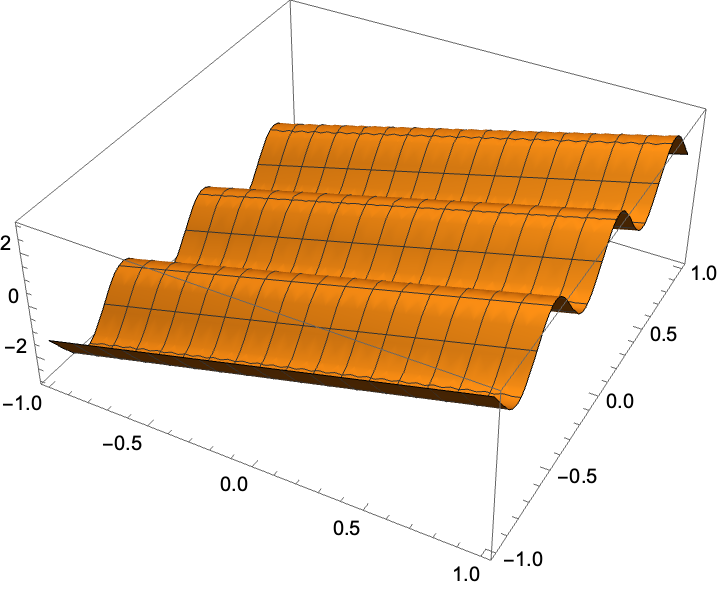
\includegraphics[width=0.275\linewidth]{Plots/s_4_1/sin(y)+2x.png} \end{center}

When we integrate a 2D function $f(x, y)$, the domain of integration needs to be a patch of area on the $xy$-plane. Perhaps the domain is a square, or a circle, or some area that is irregularly shaped. Regardless, the domain must be a \bred{2 dimensional object} on the $xy$-plane. \bred{The dimension of the domain must match the dimension of the function}.

The value of the integral over the domain corresponds to the \bred{3D volume} under the curved surface $f(x, y)$ \bred{above the domain of integration}.

\begin{center} 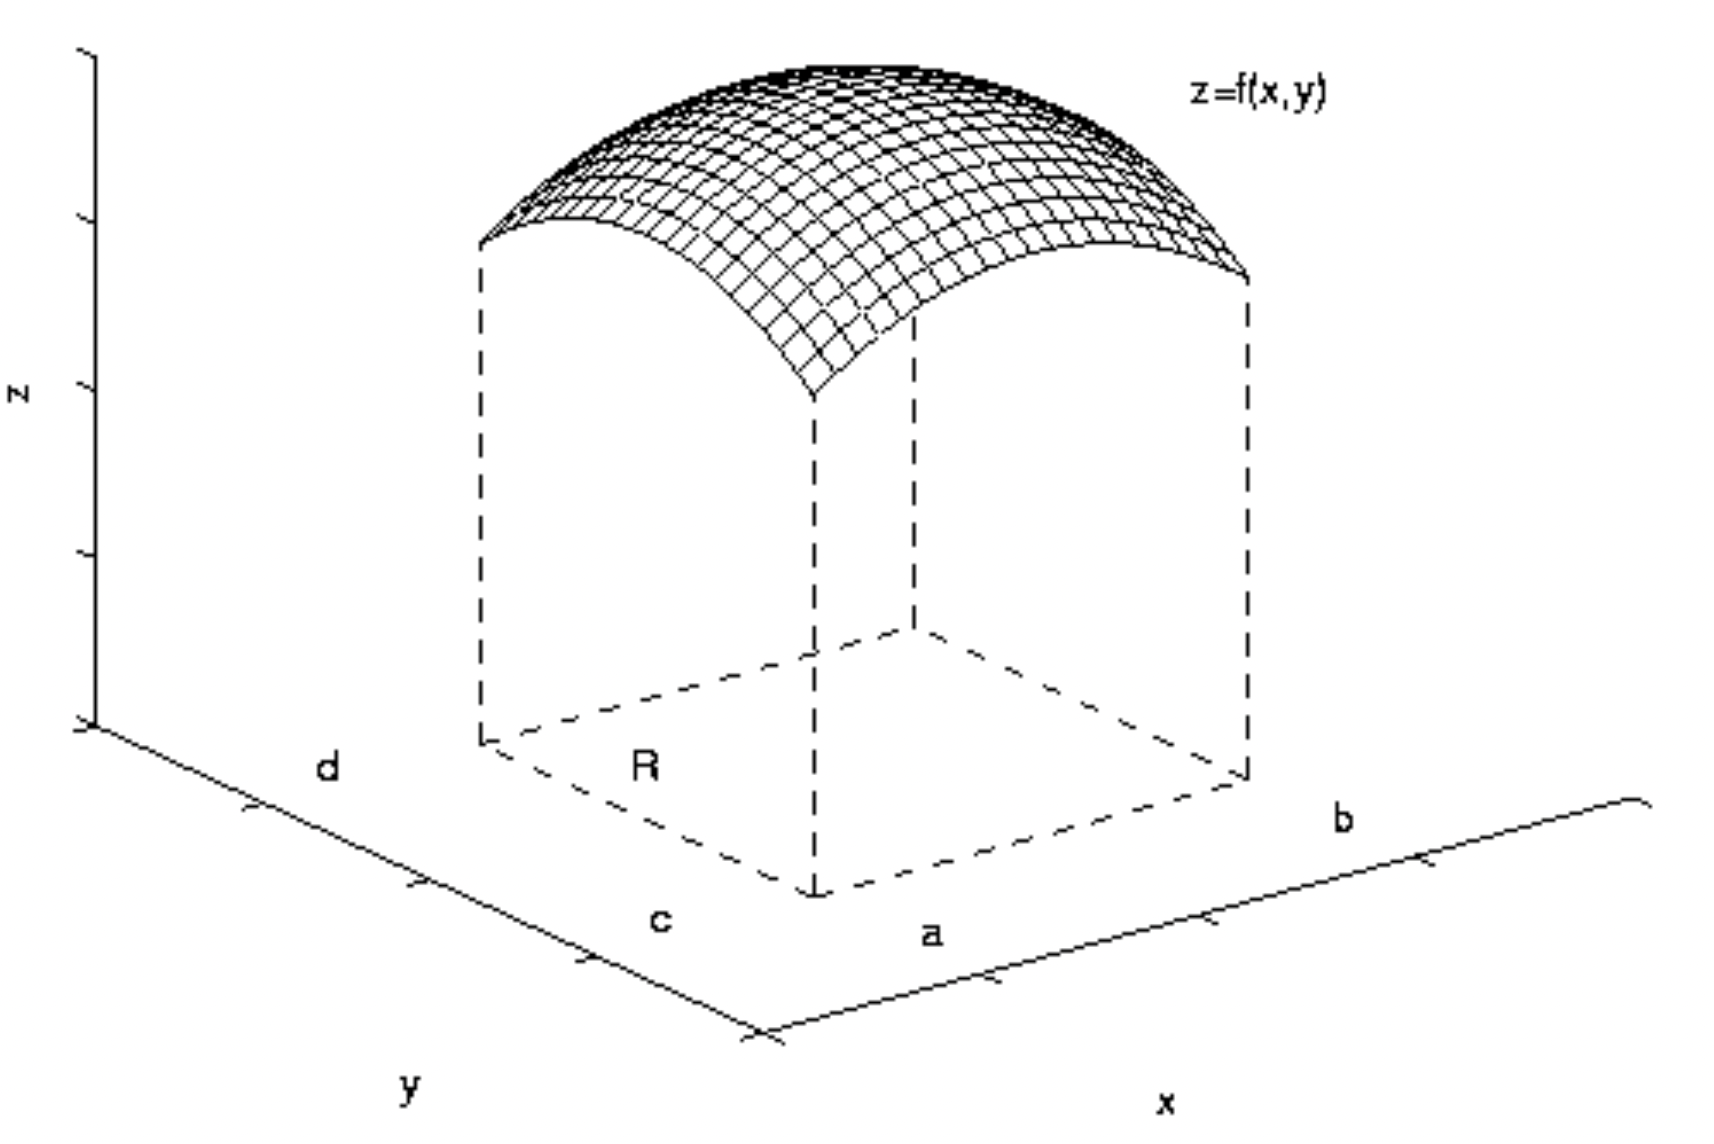
\includegraphics[width=0.75\linewidth]{Plots/s_4_1/Integral.png} \end{center}

In the above case, the domain is the rectangle on the $xy$-plane, with $x$ between $[a, b]$ and $y$ between $[c, d]$. For the volume, the base is always flat, but the top will usually be curved, since the function $z = f(x, y)$ tends to create a curved surface in 3D. If the domain had been a triangle, then the value of the integral would be the volume of a triangular prism, except the top will be curved.

Thus, when we try to integrate a 2D function $f(x, y)$ over any domain that is a 1D curve in the $xy$-plane, we would be trying to find the volume above the 1D curve. By agreeing that a curve is infinitely thin, we conclude that \itblue{the volume above the curve must be zero}. This is why our domain of integration for $f(x, y)$ \bred{must be a 2D area}.

\subsection*{Compute 2D Integrals}

A 2D integral typically will look like $$\iint_D f(x,y) = \int_D f(x, y) = \int_D f(x,y) \,dA$$ where $D$ is some 2D domain on the $xy$-plane.

To compute a 2D integral, we do not plot the function in 3D space. We split the 2D integral into 2 components, with $dx$ and $dy$.

\begin{enumerate}
    \item Draw the domain in the $xy$-plane.

    \item For all points inside the domain, determine the maximum and minimum values of $x$. These two values will be constant numbers $x_{min}$ and $x_{max}$.

    \item Pick a random value of $x$ between the minimum and maximum. Consider the vertical line that passes through the point $x$. Consider the maximum and minimum values of $y$ on the vertical line.

    \item Repeat step 3 several times. For different values of $x$ chosen, the max and min values of $y$ would be different. Typically, all the minimum values of $y$ would lie on a smooth curve, $y_{min} = m(x)$. Similarly, the maximum values would be the same, $y_{max} = M(x)$. In other words, the max and min of $y$ are \bred{functions of $x$}.

    \item Thus the integral can be evaluated as $$\int_D f(x, y) = \int_{x=x_{min}}^{x=x_{max}} \left( \int_{y=M(x)}^{y=m(x)} \,dy \right) \,dx$$ where the \bred{1D integral} inside the bracket is evaluated first. When carrying out integration with $dy$, we pretend that the variable $x$ is constant in the integration. We use the results of the inner integral, to carry out the integral outside the brackets with $dx$ afterwards.
\end{enumerate}

In the above steps, we first \bred{fix} $x$, and let $y$ vary between the lower bound curve and the upper bound curve while integrating. Then we add (integrate) all possible values of $x$.

We can also do the reverse by first attaining the min and max values of $y$ in the domain.

\begin{enumerate}
    \item Draw the domain in the $xy$-plane.

    \item For all points inside the domain, determine the maximum and minimum values of $y$. These two values will be constant numbers $y_{min}$ and $y_{max}$.

    \item Pick a random value of $y$ between the minimum and maximum. Consider the horizontal line that passes through the point $y$. Consider the maximum and minimum values of $x$ on the horizontal line. 

    \item Repeat step 3 several times. For different values of y chosen, the max and min values of x would be different. Typically, all the minimum values of x would lie on a smooth curve, xmin = m(y). Similarly, the maximum values would be the same, $x_{max} = M(y)$. In other words, the max and min of $x$ are \bred{functions of $y$}.

    \item Thus the integral can be evaluated as $$\int_D f(x, y) = \int_{y=y_{min}}^{y=y_{max}} \left( \int_{x=M(y)}^{x=m(y)} \,dx \right) \,dy$$ where the \bred{1D integral} inside the bracket is evaluated first. 
    
    Notice in the inner integral, $x$ is integrated first, and $y$ is regarded as constant. Here, $y$ is integrated after $x$, whereas in the previous way, $x$ is integrated after $y$. This is sometimes called \itblue{changing the order of integration}.

    This is not a good name since, when the order is changed, the limits of integrating are almost \bred{never the same}. In fact, the outer integral would always have limits that are constant numbers.
\end{enumerate}

Fubini's Theorem tells us that the 2 results will always be the same regardless of the order we choose, so we are free to choose the order of integration to our convenience when calculating 2D integrals \footnote{Fubini's Theorem requires all relevant integrals to be integrable. Typically no division by zero will ensure the function is integrable. }. 

Sometimes this may be used to our advantage, as some functions do not have 1D antiderivatives.

\subsection*{Properties of Integrals}

For integrals over some domain $D$ in $\mathbb{R}^n$ with integrable functions 

{~~~}

\begin{itemize}
    \item $\int_D(f + g) = \int_D f + \int_D g$ and $\int_D cf = c \int_D f$.
    
    \item If $f \le g$ on all of $D$, then $\int_D f \le \int_D g$. 
    
    \item $|f|$ is integrable and $\left| \int_D f \right| = \int_D |f|$. 

    \item If domain $C$ is contained in $D$ and $f \ge 0$, then $\int_C f \le \int_D f$. 
    
    \item For domain $C$ and $D$ (that we usually see), $\int_{C \cup D} f = \int_C f + \int_D f - \int_{C \cap D} f$. 
\end{itemize}

Notice that all properties of integral are shared with the integral in 1D.

\subsection*{Sharp Points on the Boundary of Domain}

In the case where the domain has a sharp point in the boundary, we can split up domain at the sharp point into 2 pieces, and integrate the 2 pieces separately, then add up the answers.

\subsection*{$n$-dimensional Volume}

For any set $D$ in $\mathbb{R}^n$, define the $n$-dimensional volume of $D$ $$V = \int_D 1$$ (Note: here $f = 1$, the constant function). 

\begin{itemize}
    \item If $n = 1$, then $V$ is the length of $D$ (1D interval with 1-dimensional volume). 
    \item If $n = 2$, then $V$ is the area of $D$ (2D area with 2-dimensional volume). 
    \item If $n = 3$, then $V$ is the volume of $D$ (3D volume with 3-dimensional volume). 
\end{itemize}

\begin{example}
    Let $f(x, y) = 10$. Let $D$ be the unit square between $0$ and $1$. 
    
    By noticing that the function is constant, we can see that the plot in 3D space will be a flat surface. The integral will represent the \bred{volume of the rectangular prism}, which can be calculated as base area $\times$ height. Thus, the answer will be $10 \cdot 1 = 10$.

    We can also evaluate the integral using the above steps.

    Drawing the domain, we see that the min and max values of $x$ is $0$ and $1$. For any fixed value of $x$, we see that the min and max values of $y$ is $0$ and $1$.

    % TODO: finish the graph
    \begin{center}
        \begin{tikzpicture}
                \draw[->] (-0.7, 0) -- (1.7, 0) node[right] {$x$};
                \draw[->] (0, -0.7) -- (0, 1.7) node[above] {$y$};

                \draw[DarkGreen] (0,0) rectangle (1,1);
        \end{tikzpicture}
    \end{center}
    \begin{align*}
        \int_D f(x,y)   = \int_D 10
                        = 10 \cdot \left( \int_D 1 \right)
                        = 10 \cdot \int_{x=0}^{x=1} \left( \int_{y=0}^{y=1} 1 \,dy \right) \,dx
                      & = 10 \cdot \int_{x=0}^{x=1} 1 \,dx                                      \\
                      & = 10
    \end{align*}
\end{example}

\begin{example}
    Let $f(x, y) = x$. Let $D$ be the triangle with vertices $(0, 0)$, $(1, 0)$, $(1, 2)$.

    Drawing the domain, The min and max values of $x$ is $0$ and $1$. For any fixed value of $x$, the min value of $y$ is $0$.

    However, the max value of $y$ changes. The max value of $y$ all lie on the curve $y = 2x = M(x)$.
    
    % TODO: finish the graph
    \begin{center}
        \begin{tikzpicture}
                \draw[->] (-0.7, 0) -- (1.7, 0) node[right] {$x$};
                \draw[->] (0, -0.7) -- (0, 2.7) node[above] {$y$};

                \draw[thick,DarkGreen] (0,0) -- (1,0);
                \draw[thick,DarkGreen] (1,0) -- (1,2);
                \draw[thick,DarkGreen] (1,2) -- (0,0);

                \draw[yellow] (0.33,-0.2) -- (0.33,2.2);
                \draw[yellow] (0.67,-0.2) -- (0.67,2.2);
        \end{tikzpicture}
    \end{center}
    \begin{align*}
        \int_D f(x,y)   = \int_D x
                        = \int_{x=0}^{x=1} \left( \int_{y=0}^{{\color{red}y=2x}} x \,dy \right) \,dx
                      & = \int_{x=0}^{x=1} x \left( \int_{y=0}^{{\color{red}y=2x}} 1 \,dy \right) \,dx \\
                      & = \int_{x=0}^{x=1} x \left( y \bigg|_{y=0}^{{\color{red}y=2x}} \right) \,dx    \\
                      & = \int_{x=0}^{x=1} x \cdot 2x \,dx                                             \\
                      & = \int_{x=0}^{x=1} 2x^2
                        = \frac{2}{3} x^3 \bigg|_{x=0}^{x=1}
                        = \frac{2}{3}
    \end{align*}

    Notice that the bound inside the inner integral is a function of $x$. Since we are integrating with $dy$, we regard $x$ as constant, and move it out of the integral.
\end{example}

\subsection*{Domain Defined Using Inequalities}

When domains are defined using an inequality, we take the inequality and make it equality. This will create a curve in the $xy$-plane which we can draw. We start on the curve, and move a little bit to the right of the curve. This increased the value of $x$, so one side of the equality has become larger. Using this information, we can determine the area defined by the equality.

\begin{example}
    Let $f(x, y)$ be a function. Let $D$ be bounded by $y = x$ and $y = x^2$.

    \begin{center}
        \begin{tikzpicture}
            \draw[->] (-2.2,0) -- (2.7,0) node[right] {$x$};
            \draw[->] (0,-1.2) -- (0,2.7) node[above] {$y$};

            \draw[thick,blue,domain=-1:3] plot (\x, {\x}) node[below right] {$y=x$};
            \draw[thick,DarkGreen,domain=-2:2.5] plot (\x, {((\x)^2)/2}) node[left] {$y=x^2$};

            \draw[dashed] (2,2) -- (2,0) node[below] {$1$};
            \draw[dashed] (2,2) -- (0,2) node[left] {$1$};
        \end{tikzpicture}
    \end{center}

    After drawing the curve, we see that the intersection is at $(0, 0)$ and $(1, 1)$. We see that the min value of $y$ lies on the curve $y = x^2 = m(x)$. The max value of $y$ is $y = x = M(x)$.
    $$\int_D f(x, y) = \int_{x=0}^{x=1} \left( \int_{y=x^2}^{y=x} f(x, y) \,dx \right) \,dy$$
\end{example}

\begin{example}
    Let $D$ be bounded by $y = x$ and $y = -x + 2$, $y = 0$.

    The max value of $y$ is not a smooth curve due to the sharp point at $x = 1$. We can split the integral in 2 pieces, with $x \in [0, 1]$, and $x \in [1, 2]$.
    $$\int_D f(x, y) = \int_{x=0}^{x=1} \left( \int_{y=0}^{y=x} f(x, y) \,dy \right) + \int_{x=1}^{x=2} \left( \int_{y=0}^y={-x+2} f(x, y) \,dy \right)$$

    We can also interchange the order of integration.
\end{example}

\begin{exercise}
    Let $D$ be bounded by $y = x$ and $y = -x + 2$, $y = 0$.

    Compute the integral by changing the order of integration. Compare with example 4.4, notice that we no longer need to split up the domain, because the sharp point is now the endpoint of the integral.
\end{exercise}

\begin{exercise}
    Integrate $\int_D f(x, y)$. 

    \begin{enumerate}
        \item Let $D$ be bounded by $x = 0$, $y = 0$, $y = -2x + 2$. 
        \item Let $D$ be bounded by $y = x + 1$, $y = -x^2 + 1$.
        \item Let $D$ be the triangle defined by $(0, 2)$, $(0, -2)$, $(2, 0)$.
        \item Let $D = \{ (x, y) \in \mathbb{R}^2 | x \in [0, 1], y \in [0, 1], y > x^2 \}$
    \end{enumerate}
\end{exercise}

\begin{exercise}
    Evaluate $$\int_{y=0}^{y=1} \left( \int_{x=0}^{x=y^4} y \frac{\sin{x}}{(1 - \sqrt{x})} \,dx \right) \,dy$$

    \textbf{Strategy:}

    The function looks difficult. What is the region of integration? Try changing the order of integration.
\end{exercise}

\begin{exercise}
    Evaluate

    {~~~}

    \begin{enumerate}
        \item $\int_{x=0}^{x=8} \left( \int_{y=\sqrt[3]{x}}^{y=2} \frac{x}{y^7 +1} \,dy \right) \,dx$
        \item $\int_{x=0}^{x=4} \left( \int_{y=\sqrt{x}}^{y=2} y \cos(y^4 + 3) \,dy \right) \,dx$
        \item $\int_{y=0}^{y=1} \left( \int_{x=y}^{x=\sqrt{y}} \frac{\sin{x}}{x} \,dx \right) \,dy$
        \item $\int_{y=0}^{y=1} \left( \int_{x=0}^{x=arccos{y}} e^{2\sin{x}} \,dx \right) \,dy$
    \end{enumerate}
\end{exercise}

\section{Regular Integral in 3D}

To compute integral of $f(x,y,z)$ over a 3 dimensional domain $D$, it is similar.

\begin{enumerate}
    \item Draw the domain in 3D. (This is difficult). 

    \item Take the \bred{projection} of the 3D domain onto one of the 3 planes created by the axis. This creates a 2D domain. Suppose in this case, we take the projection onto the $xy$-plane.
    
    \item Compute the limits of integration for the 2D domain in $xy$-plane (as a 2D integral). These will be the limits of the outer most integrals. Match $dx$ and dy according to the order used. 
    
    \item Pick a random point $(x, y)$ in the projection. Consider the \bred{vertical} line in the $z$ direction. Consider the maximum and minimum values of $z$. 
    
    \item Repeat step $4$ several times. The min and max values of $z$ usually will be on a smooth surface that depend on the point $(x, y)$. Thus $z_{min} = m(x, y)$ and $z_{max} = M(x, y)$.
    
    These are the limits of the inner most integral, with $dz$.
    $$\int_D f(x, y, z) = \int_{2D} \left( \int_{z=m(x,y)}^{z=M(x,y)} f(x, y, z) \,dz \right) \,dx \,dy$$
    where the order of $dx \,dy$ depends upon the order chosen for the 2D integral. In general, inner limits can depend on variables from outer integrals, but limits of outer integrals never depend on variables from inner integrals. 
\end{enumerate}

When an equation involves only 2 variables (in 3D), it gives a curve in 2D which extends infinitely toward the 3rd dimension, giving a cylinder-like surface in 3D. With 2 such curves, we will get at least 2 intersection points. Connecting the intersection points with a ``smooth'' curve typically gives the picture of the domain in 3D.

\begin{example}
    Let $D$ be bounded by the given equations, in first octant. 

    Compute the integral $\int_D f(x, y, z)$ in 6 ways (3 ways to project, 2 ways to compute the 2D integral of the projection). 

    \begin{minipage}[t]{0.45\linewidth}
        \begin{enumerate}
            \item $z = 1 - x$, $y = 1$
            \item $z = 1 - y$, $x = y^2$
            \item $z = 1 - x^2$, $y = 1 - x$
        \end{enumerate}
    \end{minipage}
    \begin{minipage}[t]{0.45\linewidth}
        \begin{enumerate} \setcounter{enumi}{3}
            \item $z = 1 - y^2$, $y = x$
            \item $y^2 + z^2 = 9$, $y = 3x$
            \item $2x + y + 2z = 1$
        \end{enumerate}
    \end{minipage}
\end{example}

%----------------------------------------------------------------------------------------
%	APPENDICES
%----------------------------------------------------------------------------------------

\part{Appendices}

\chapterimage{sol.png}

\chapter*{Solutions to Exercise Questions}
\addcontentsline{toc}{chapter}{\textcolor{ocre}{A Solutions to Exercise Questions}}
\setlength{\parindent}{0pt} % No indentation

\section*{Chapter 1}

\subsection*{Exercise 1.1}

\begin{enumerate}
    \item
    \begin{minipage}[t]{0.45\linewidth}
        $x = 2y^2$
    \end{minipage}
    \begin{minipage}[t]{0.45\linewidth}
        \begin{center}
            \tikzsetnextfilename{c01e01-01}%
            \begin{tikzpicture}[baseline=(current bounding box.west)]
                \draw[->] (-0.5, 0) -- (2.5, 0) node[right] {$x$};
                \draw[->] (0, -1.5) -- (0, 1.5) node[above] {$y$};

                \draw[thick,blue,domain=0:2] plot (\x, {sqrt(\x)});
                \draw[thick,blue,domain=0:2] plot (\x, {-sqrt(\x)});
            \end{tikzpicture}
        \end{center}
    \end{minipage}

    \item
    \begin{minipage}[t]{0.45\linewidth}
        $\begin{aligned}[t]
            \frac{x^2}{2} + \frac{y^2}{9}                                  & = 1 \\
            \left(\frac{x}{\sqrt{2}}\right)^2 + \left(\frac{y}{3}\right)^2 & = 1
        \end{aligned}$
    \end{minipage}
    \begin{minipage}[t]{0.45\linewidth}
        \begin{center}
            \tikzsetnextfilename{c01e01-02}%
            \begin{tikzpicture}[baseline=(current bounding box.west)]
                \draw[->] (-1.12, 0) -- (1.12, 0) node[right] {$x$};
                \draw[->] (0, -2) -- (0, 2) node[above] {$y$};

                \draw[thick,blue] (0, 0) ellipse (0.8cm and 1.68cm);

                \draw[thick,red] (0.8, 0.25) -- (0.8, 0) node[below,red] {$\sqrt{2}$};
                \draw[thick,red] (-0.8, 0.25) -- (-0.8, 0) node[below,red] {$-\sqrt{2}$};
                \draw[thick,red] (0.25, 1.68) -- (0, 1.68) node[left,red] {$3$};
                \draw[thick,red] (0.25, -1.68) -- (0, -1.68) node[left,red] {$-3$};
            \end{tikzpicture}
        \end{center}
    \end{minipage}

    \item
    \begin{minipage}[t]{0.45\linewidth}
        $\begin{aligned}[t]
            x^2 + 2y^2                                                     & = 4 \\
            \frac{x^2}{4} + \frac{2y^2}{4}                                 & = 1 \\
            \left(\frac{x}{2}\right)^2 + \left(\frac{y}{\sqrt{2}}\right)^2 & = 1
        \end{aligned}$
    \end{minipage}
    \begin{minipage}[t]{0.45\linewidth}
        \begin{center}
            % \tikzsetnextfilename{c01e01-03}%
            \begin{tikzpicture}[baseline=(current bounding box.north)]
                \draw[->] (-1.92, 0) -- (1.92, 0) node[right] {$x$};
                \draw[->] (0, -1.44) -- (0, 1.44) node[above] {$y$};

                \draw[thick,blue] (0, 0) ellipse (1.6cm and 1.12cm);

                \draw[thick,red] (1.6, 0.25) -- (1.6, 0) node[below,red] {$2$};
                \draw[thick,red] (-1.6, 0.25) -- (-1.6, 0) node[below,red] {$-2$};
                \draw[thick,red] (0.25, 1.12) -- (0, 1.12) node[left,red] {$\sqrt{2}$};
                \draw[thick,red] (0.25, -1.12) -- (0, -1.12) node[left,red] {$-\sqrt{2}$};
            \end{tikzpicture}
        \end{center}
    \end{minipage}

    \item
    \begin{minipage}[t]{0.45\linewidth}
        $\begin{aligned}[t]
            x^2 + 3y^2 + 2x - 12y + 10                                             & = 0 \\
            (x^2 + 2x + 1) + 3(y^2 - 4y + 4) - 3                                   & = 0 \\
            (x + 1)^2 + 3(y - 2)^2                                                 & = 3 \\
            \left(\frac{x + 1}{\sqrt{3}}\right)^2 + \left(\frac{y - 2}{1}\right)^2 & = 1
        \end{aligned}$

        Ellipse before the shift (in {\color{DarkGreen}green}): $$\left(\frac{x}{\sqrt{3}}\right)^2 + \left(\frac{y}{1}\right)^2 = 1$$

        Then, shift $1$ unit left and $2$ units up.
    \end{minipage}
    \begin{minipage}[t]{0.45\linewidth}
        \begin{center}
            \tikzsetnextfilename{c01e01-04}%
            \begin{tikzpicture}[baseline=(current bounding box.north)]
                \draw[->] (-3.2, 0) -- (2.2, 0) node[right] {$x$};
                \draw[->] (0, -1.2) -- (0, 3.7) node[above] {$y$};

                \draw[thick,DarkGreen] (0, 0) ellipse (1.7cm and 1cm);
                \draw[thick,blue] (-1, 2) ellipse (1.7cm and 1cm);

                \draw[thick,orange] (1.7, 0.25) -- (1.7, 0) node[below] {$\sqrt{3}$};
                \draw[thick,orange] (0.25, 1) -- (0, 1) node[left,red] {$1$};

                \draw[thick,red,dashed] (0.7, 2) -- (0.7, 0) node[below] {$\sqrt{3} - 1$};
                \draw[thick,red,dashed] (-2.7, 2) -- (-2.7, 0) node[below] {$-\sqrt{3} - 1$};

                \draw[thick,red,dashed] (-1, 2) -- (0, 2) node[left] {$2$};
                \draw[thick,red,dashed] (-1, 2) -- (-1, 0) node[below] {$-1$};

                \draw[thick,red,dashed] (-1, 3) -- (0, 3) node[left] {$3$};
                \draw[thick,red,dashed] (-1, 1) -- (0, 1);
            \end{tikzpicture}
        \end{center}
    \end{minipage}

    \item
    \begin{minipage}[t]{0.45\linewidth}
        $y^2 - x^2 = 1$

        {~~~}

        If $y = 0$, then $-x^2 = 1$, not possible.

        Thus, the graph must not cross the horizontal axis, and the hyperbola opens \bred{up and down}.

        {~~~}

        If $x = 0$, then $y^2 = 1$, $y = \pm 1$.
    \end{minipage}
    \begin{minipage}[t]{0.45\linewidth}
        \begin{center}
            \tikzsetnextfilename{c01e01-05}%
            \begin{tikzpicture}[baseline=(current bounding box.north)]
                \draw[->] (-2.2, 0) -- (2.2, 0) node[right] {$x$};
                \draw[->] (0, -2.2) -- (0, 2.2) node[above] {$y$};

                \clip(-2, -2) rectangle (2, 2);

                \draw[thick,blue,rotate around={90:(0,0)},domain=-0.99:0.99] plot ({( 1+(\x)^2)/(1-(\x)^2)}, {  2 *(\x)/(1-(\x)^2)});
                \draw[thick,blue,rotate around={90:(0,0)},domain=-0.99:0.99] plot ({(-1-(\x)^2)/(1-(\x)^2)}, {(-2)*(\x)/(1-(\x)^2)});

                \draw[red] (0.25,-1) -- (0,-1) node[left] {$-1$};
                \draw[red] (0.25,1) -- (0,1) node[left] {$1$};
            \end{tikzpicture}
        \end{center}
    \end{minipage}

    \item
    \begin{minipage}[t]{0.45\linewidth}
        $\begin{aligned}[t]
            \frac{(x-2)^2}{4} - \frac{(y+2)^2}{9}                       & = 1 \\
            \left(\frac{x-2}{2}\right)^2 - \left(\frac{y+2}{3}\right)^2 & = 1
        \end{aligned}$

        {~~~}

        Hyperbola before the shift (in {\color{DarkGreen}green}): $$\left(\frac{x}{2}\right)^2 - \left(\frac{y}{3}\right)^2 = 1$$

        If $x = 0$, then $-y^2 = 1$, not possible.

        Thus, the graph must not cross the vertical axis, and the hyperbola opens \bred{left and right}.

        If $y = 0$, then $\left(\frac{x}{2}\right)^2 = 1$, $x = \pm 2$.
    \end{minipage}
    \begin{minipage}[t]{0.45\linewidth}
        \begin{center}
            \tikzsetnextfilename{c01e01-06}%
            \begin{tikzpicture}[baseline=(current bounding box.north)]
                \draw[->] (-2.2, 0) -- (3.2, 0) node[right] {$x$};
                \draw[->] (0, -2.7) -- (0, 2.7) node[above] {$y$};

                \clip(-3, -2.5) rectangle (3, 2);

                \draw[thick,DarkGreen,domain=-0.99:0.99] plot ({( 1+(\x)^2)/(1-(\x)^2)}, {  2 *(\x)/(1-(\x)^2)});
                \draw[thick,DarkGreen,domain=-0.99:0.99] plot ({(-1-(\x)^2)/(1-(\x)^2)}, {(-2)*(\x)/(1-(\x)^2)});

                \draw[thick,blue,domain=-0.99:0.99] plot ({( 1+(\x)^2)/(1-(\x)^2) + 1}, {  2 *(\x)/(1-(\x)^2) - 1});
                \draw[thick,blue,domain=-0.99:0.99] plot ({(-1-(\x)^2)/(1-(\x)^2) + 1}, {(-2)*(\x)/(1-(\x)^2) - 1});

                \draw[thick,red,dashed] (2,-1) -- (0,-1) node[left] {$-2$};
                \draw[thick,red,dashed] (2,-1) -- (2,0) node[below] {$4$};
                \draw[thick,red,dashed] (1,0) -- (1,-1) node[below] {$(2,-2)$};

                \draw[orange] (-1,0.25) -- (-1,0) node[below] {$-2$};
                \draw[orange] (1,0.25) -- (1,0) node[below] {$2$};
            \end{tikzpicture}
        \end{center}
    \end{minipage}
\end{enumerate}

\subsection*{Exercise 1.2}

\begin{enumerate}
    \item
    \begin{minipage}[t]{0.25\linewidth}
        $\begin{aligned}[t]
            x^2 + y^2 & = 1 \\
            r^2       & = 1 \\
            r         & = 1
        \end{aligned}$
    \end{minipage}
    \begin{minipage}[c]{0.2\linewidth}
        \begin{center}
            \begin{tikzpicture}
                \draw[->] (-1.2, 0) -- (1.2, 0) node[right] {$r_{(y)}$};
                \draw[->] (0, -1.2) -- (0, 1.2) node[above] {$z$};

                \draw[thick,blue,domain=-1:1] plot (1, \x) node[left,red] {$r = 1$};
            \end{tikzpicture}
        \end{center}
    \end{minipage}
    \begin{minipage}[c]{0.5\linewidth}
        \begin{center} 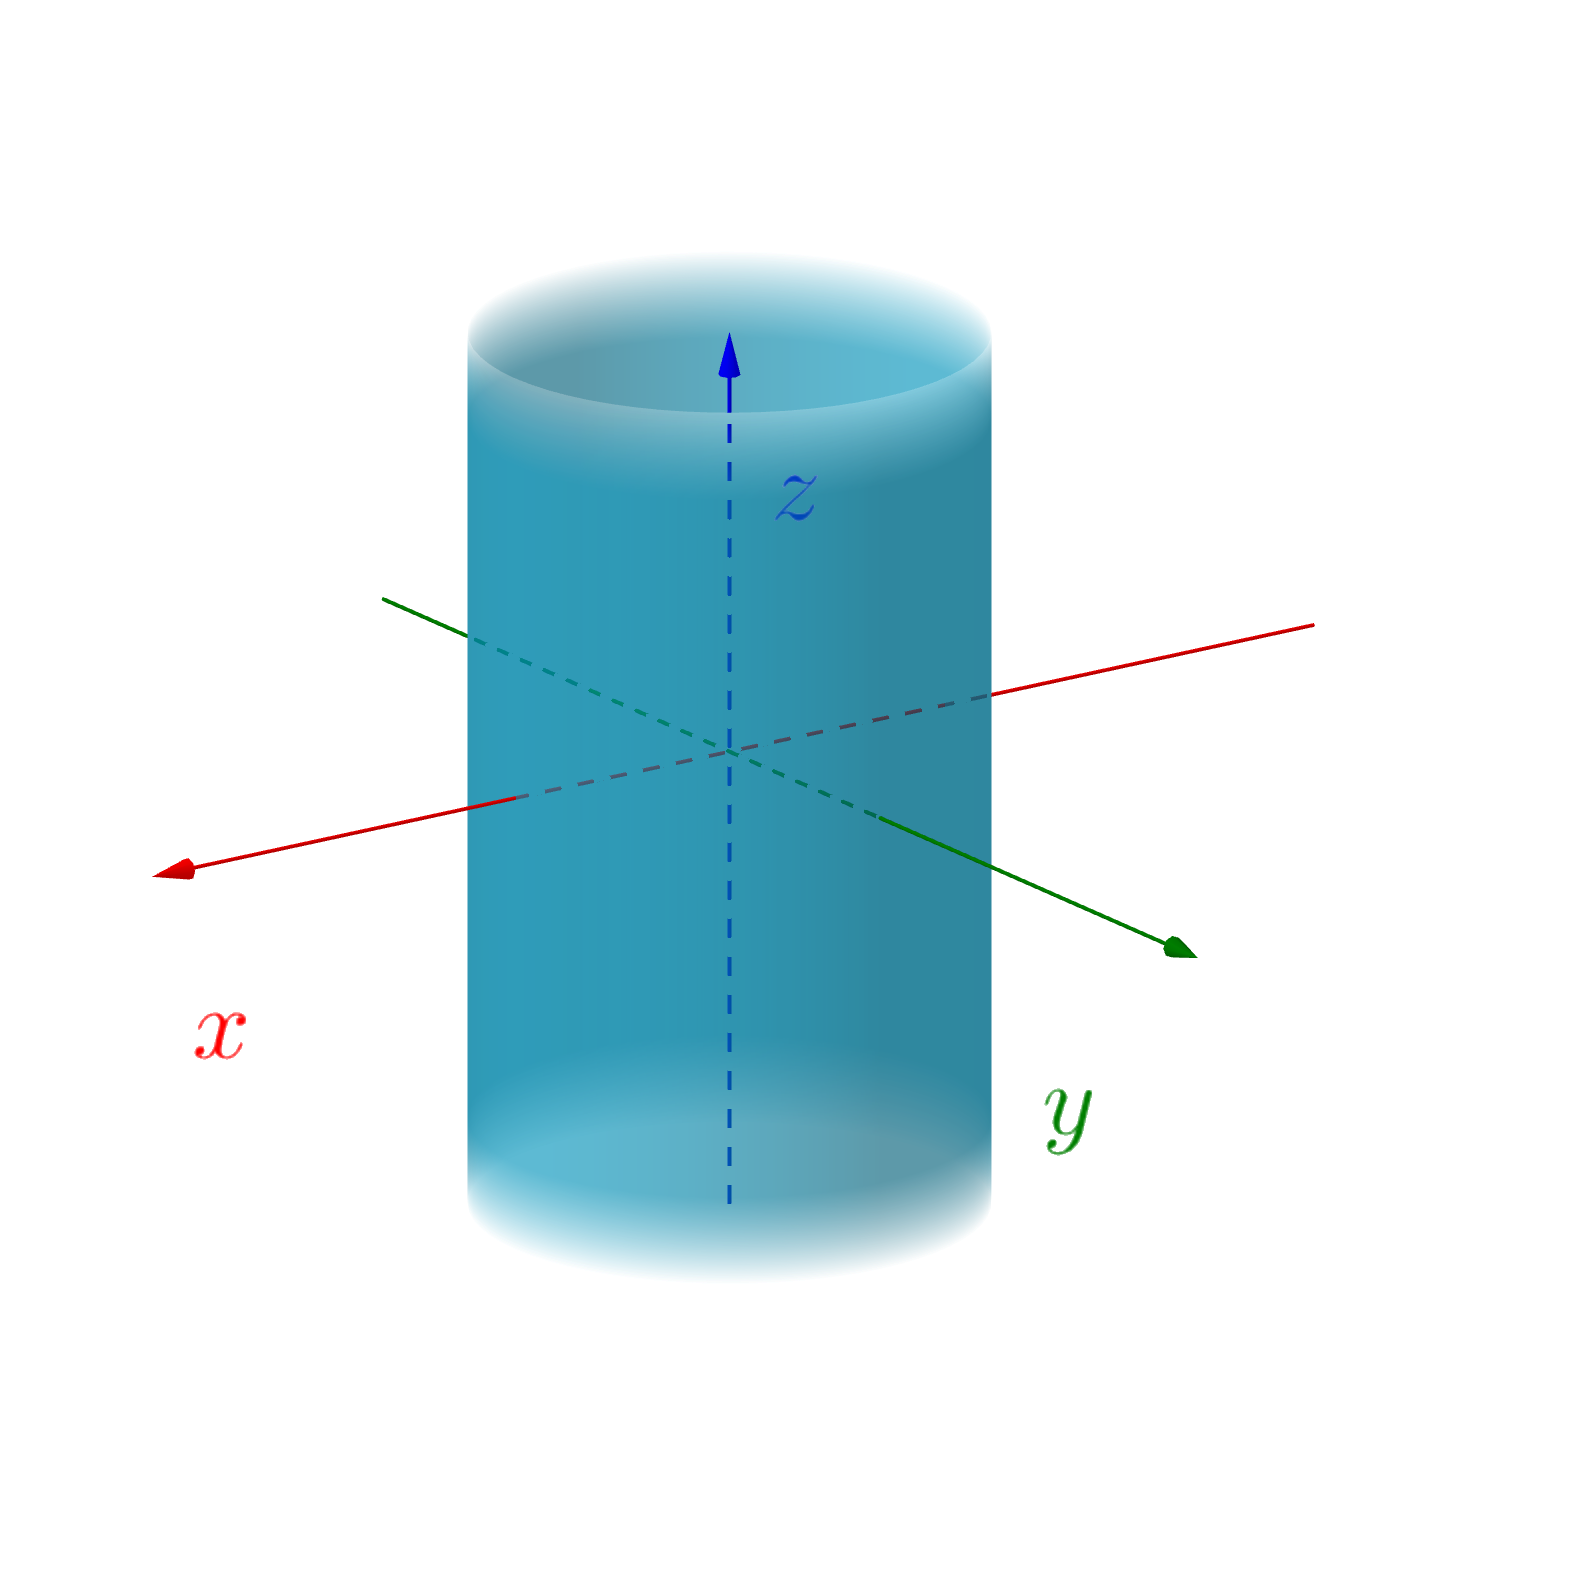
\includegraphics[width=0.9\linewidth]{Plots/e_1_2/1.png} \end{center}
    \end{minipage}

    \item
    \begin{minipage}[t]{0.25\linewidth}
        $\begin{aligned}[t]
            z & = x^2 + y^2 \\
            z & = r^2
        \end{aligned}$
    \end{minipage}
    \begin{minipage}[c]{0.2\linewidth}
        \begin{center}
            \begin{tikzpicture}
                \draw[->] (-1.2, 0) -- (1.2, 0) node[right] {$r_{(y)}$};
                \draw[->] (0, -0.7) -- (0, 1.7) node[above] {$z$};

                \draw[thick,blue,domain=0:1.25] plot (\x, {(\x)^2}) node[above,red] {$z = r^2$};
            \end{tikzpicture}
        \end{center}
    \end{minipage}
    \begin{minipage}[c]{0.5\linewidth}
        \begin{center} 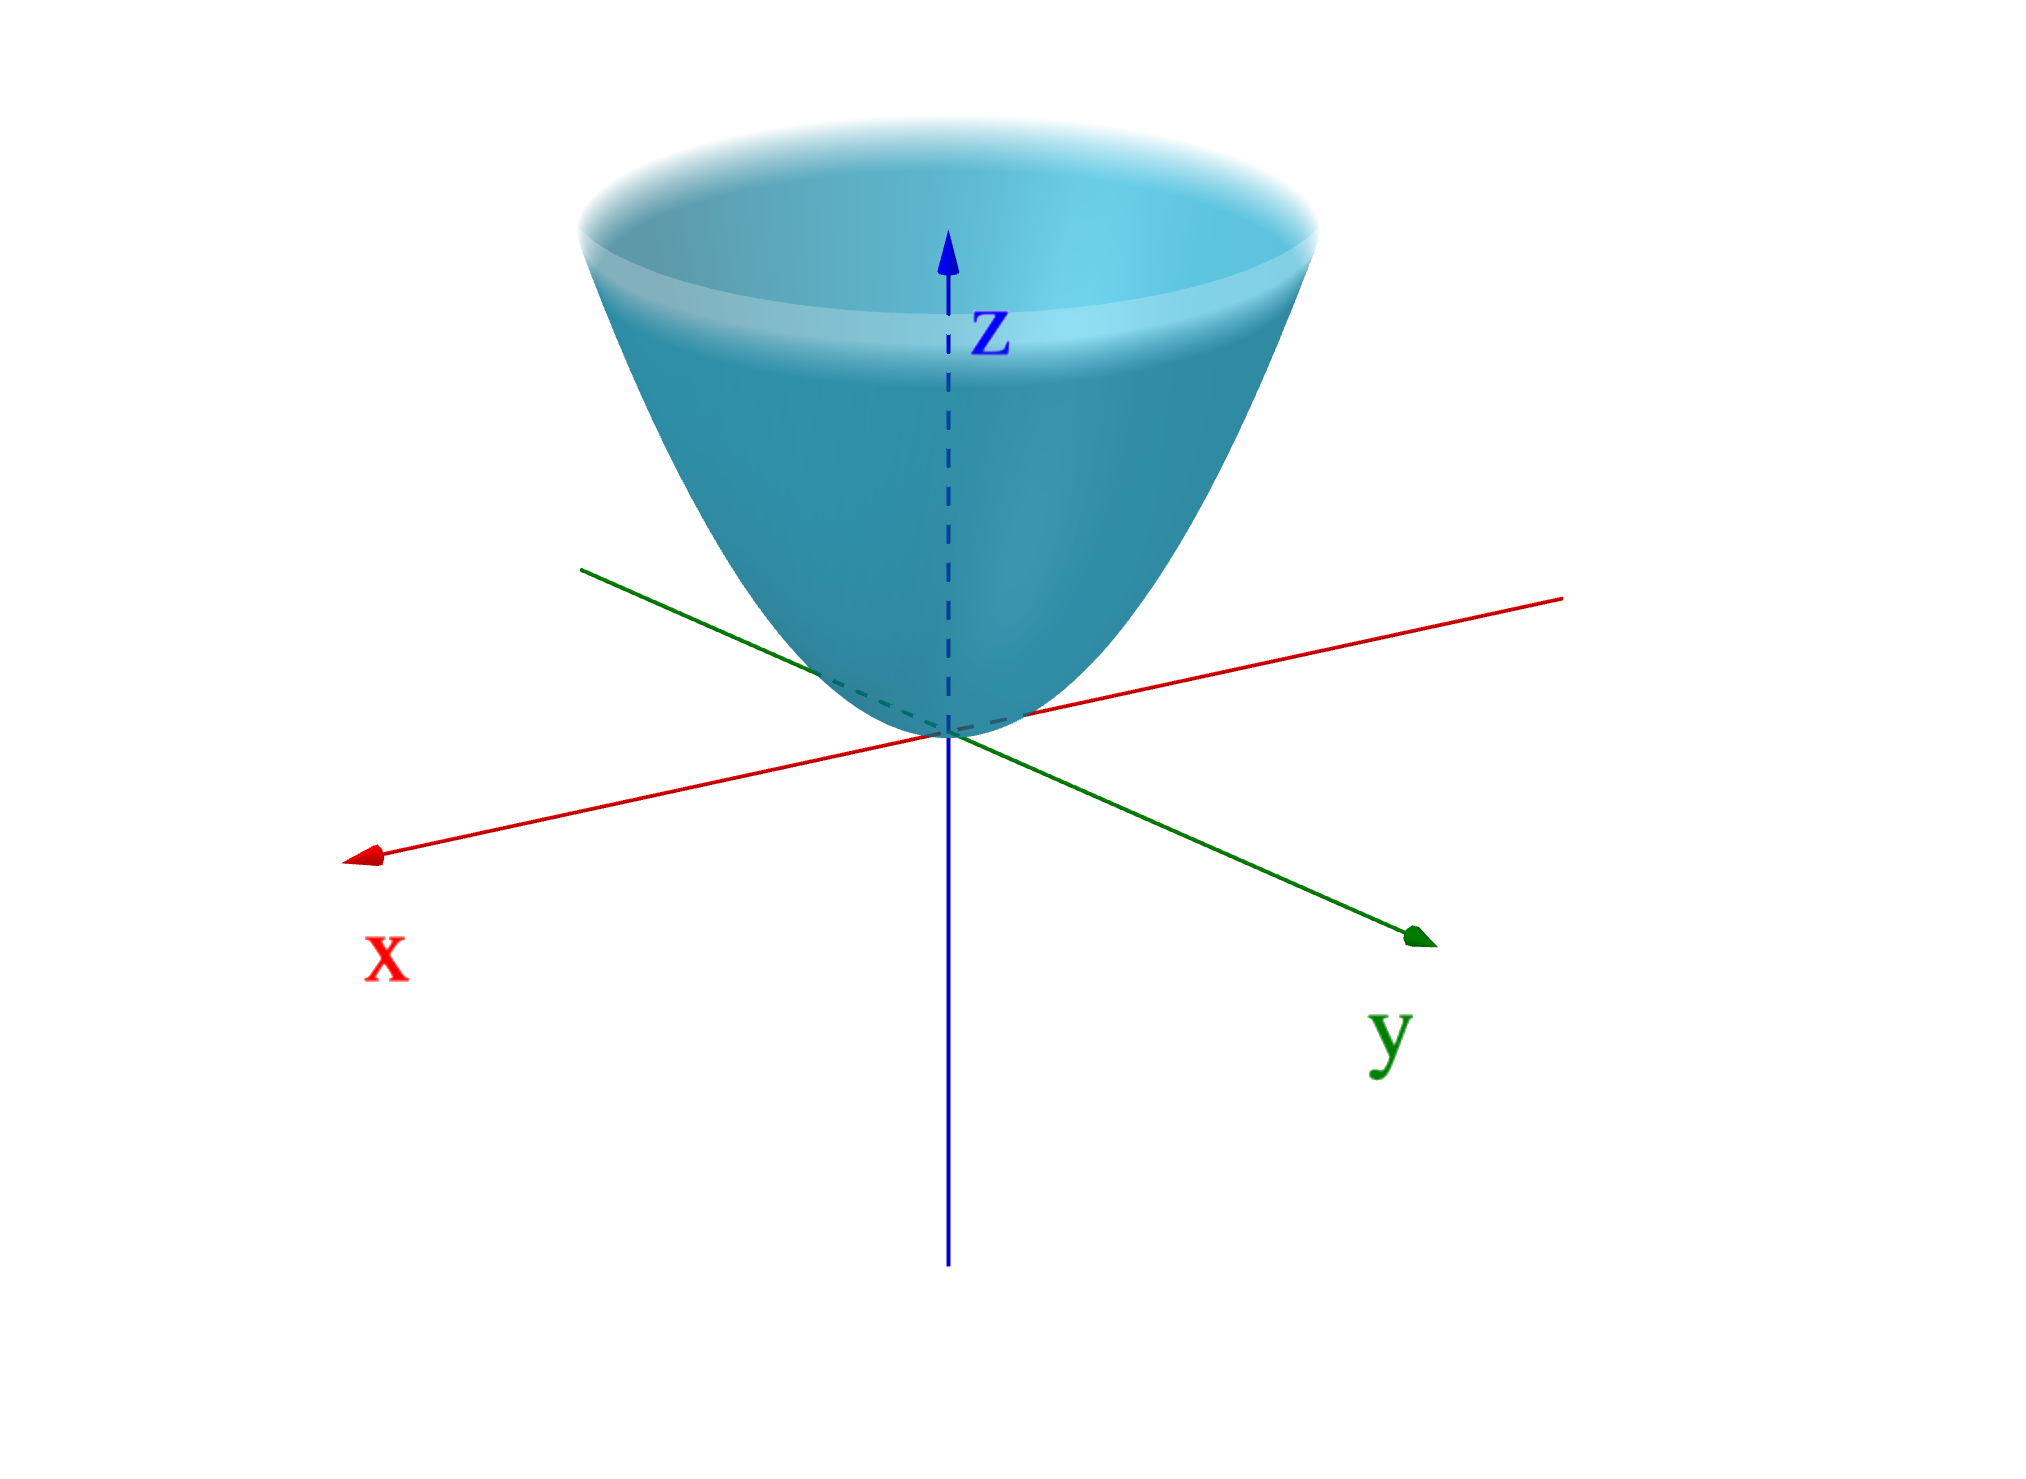
\includegraphics[width=0.9\linewidth]{Plots/e_1_2/2.png} \end{center}
    \end{minipage}

    \item
    \begin{minipage}[t]{0.25\linewidth}
        $\begin{aligned}[t]
            z^2 & = x^2 + y^2 \\
            z^2 & = r^2       \\
            z   & = \pm r
        \end{aligned}$
    \end{minipage}
    \begin{minipage}[c]{0.2\linewidth}
        \begin{center}
            \begin{tikzpicture}
                \draw[->] (-1.2, 0) -- (1.2, 0) node[right] {$r_{(y)}$};
                \draw[->] (0, -1.2) -- (0, 1.2) node[above] {$z$};

                \draw[thick,blue,domain=0:1] plot (\x, {\x});
                \draw[thick,blue,domain=0:1] plot (\x, {-\x});

                \node[red] at (-0.6,0.25) {$z = \pm r$};
            \end{tikzpicture}
        \end{center}
    \end{minipage}
    \begin{minipage}[c]{0.5\linewidth}
        \begin{center} 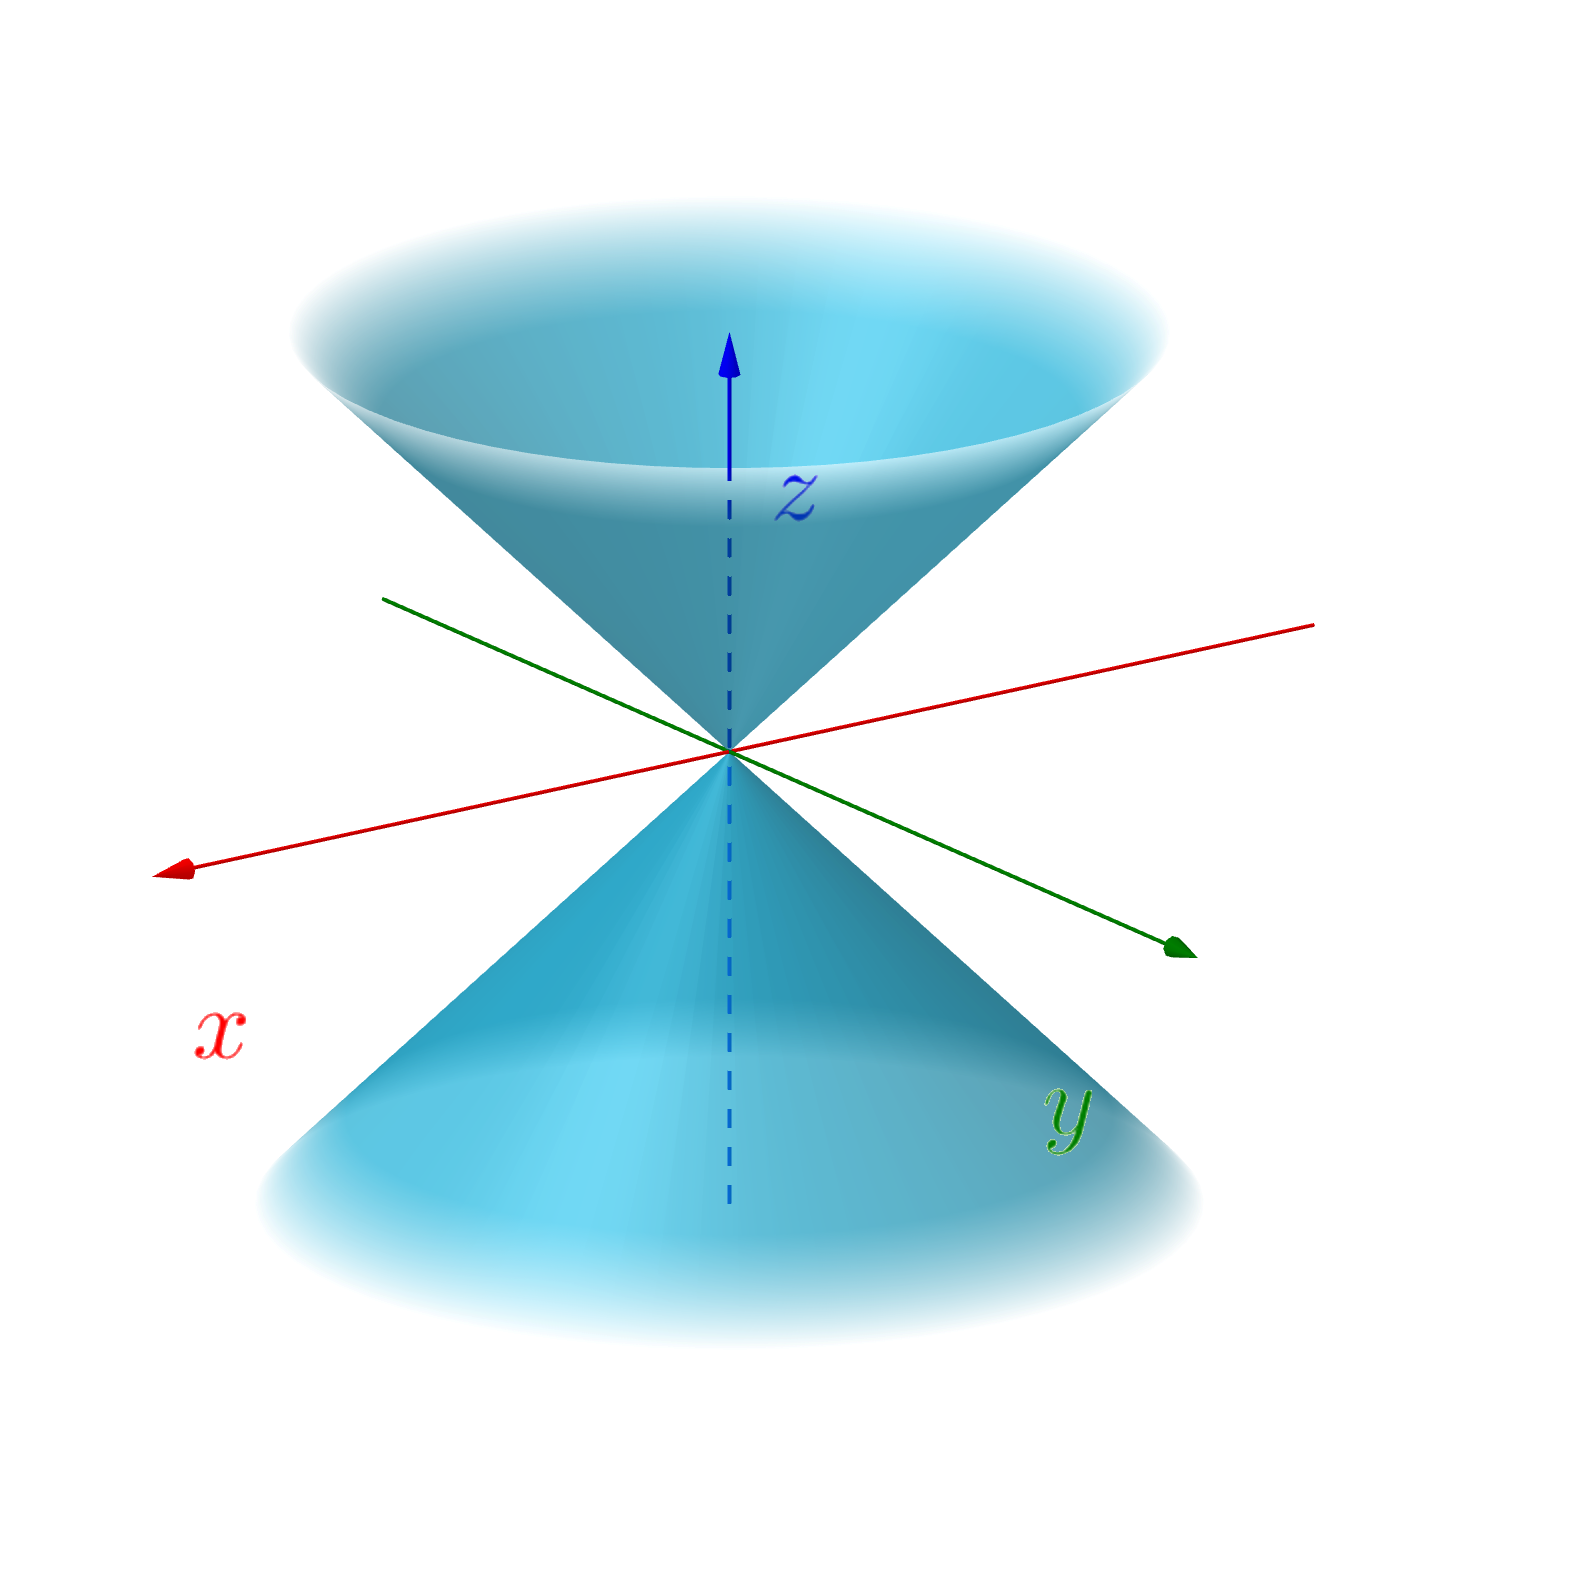
\includegraphics[width=0.9\linewidth]{Plots/e_1_2/3.png} \end{center}
    \end{minipage}

    \item
    \begin{minipage}[t]{0.25\linewidth}
        $\begin{aligned}[t]
            x^2 + y^2 + \frac{z^2}{4}                               & = 1 \\
            r^2 + \frac{z^2}{4}                                     & = 1 \\
            \left(\frac{r}{1}\right)^2 + \left(\frac{z}{2}\right)^2 & = 1
        \end{aligned}$
    \end{minipage}
    \begin{minipage}[c]{0.2\linewidth}
        \begin{center}
            \begin{tikzpicture}
                \draw[->] (-1.2, 0) -- (1.2, 0) node[right] {$r_{(y)}$};
                \draw[->] (0, -1.2) -- (0, 1.2) node[above] {$z$};

                \draw[thick,blue] (0,1) arc (90:-90:0.5cm and 1cm);

                \node[red] at (0,0.5) {$\left(\frac{r}{1}\right)^2 + \left(\frac{z}{2}\right)^2 = 1$};
            \end{tikzpicture}
        \end{center}
    \end{minipage}
    \begin{minipage}[c]{0.5\linewidth}
        \begin{center} 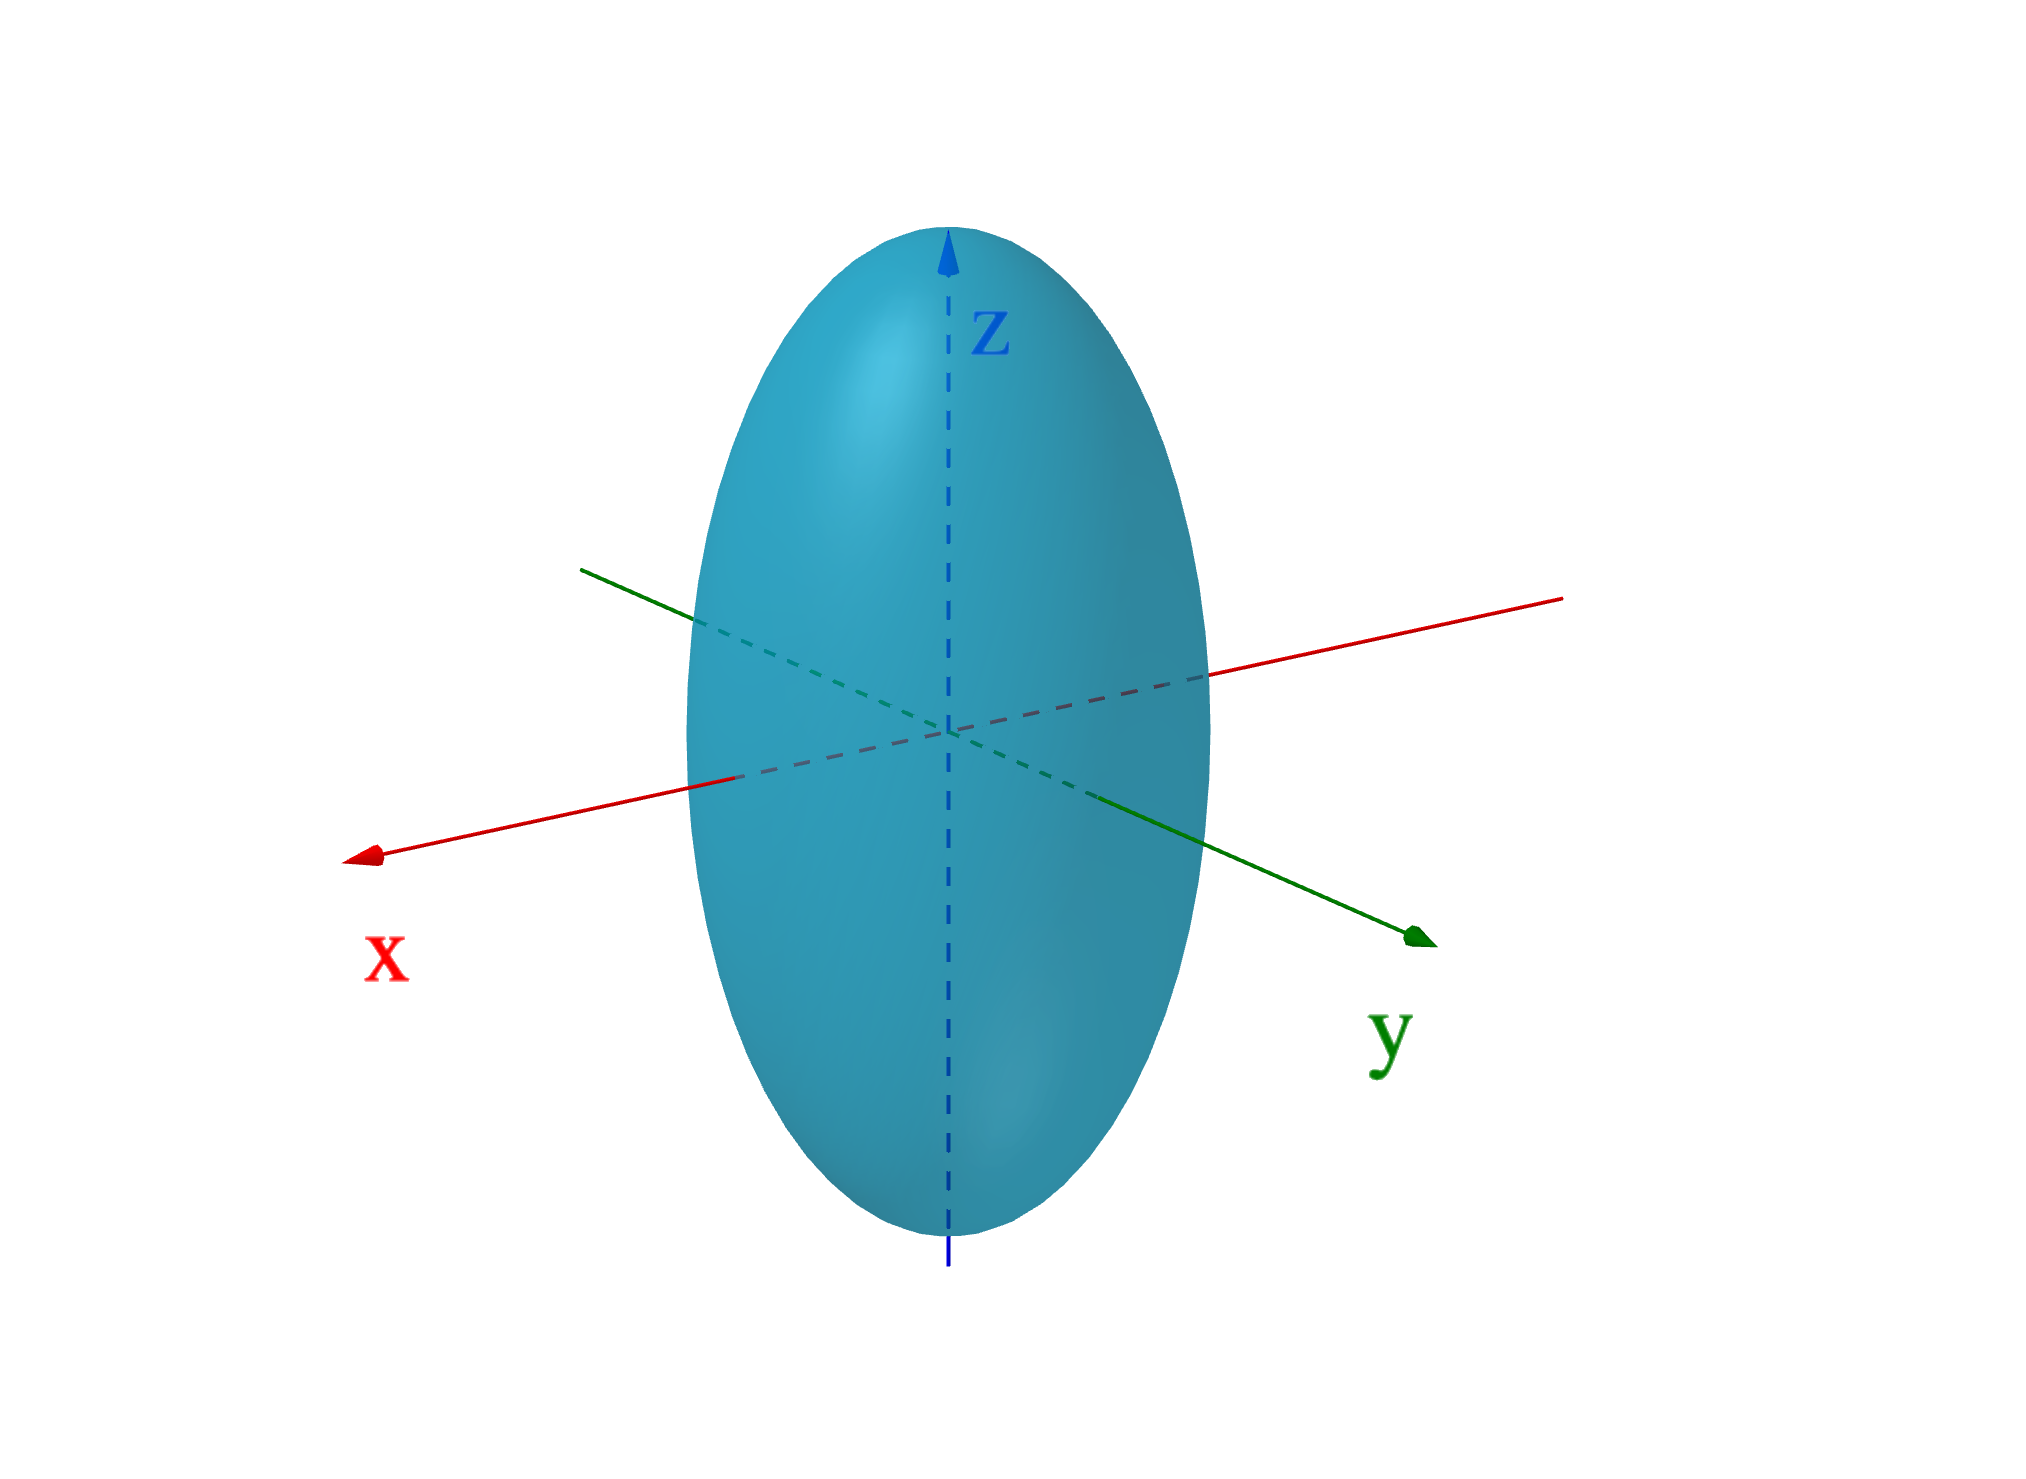
\includegraphics[width=0.9\linewidth]{Plots/e_1_2/4.png} \end{center}
    \end{minipage}

    \item
    \begin{minipage}[t]{0.25\linewidth}
        $\begin{aligned}[t]
            z & = \left(\sqrt{x^2 + y^2} - 1\right)^2 \\
            z & = (r - 1)^2
        \end{aligned}$
    \end{minipage}
    \begin{minipage}[c]{0.2\linewidth}
        \begin{center}
            \begin{tikzpicture}
                \draw[->] (-0.7, 0) -- (1.7, 0) node[right] {$r_{(y)}$};
                \draw[->] (0, -0.7) -- (0, 1.7) node[above] {$z$};

                \draw[thick,blue,domain=0:2.5] plot (\x, {(\x - 1)^2}) node[below left,red] {$z = (r - 1)^2$};
            \end{tikzpicture}
        \end{center}
    \end{minipage}
    \begin{minipage}[c]{0.5\linewidth}
        \begin{center} 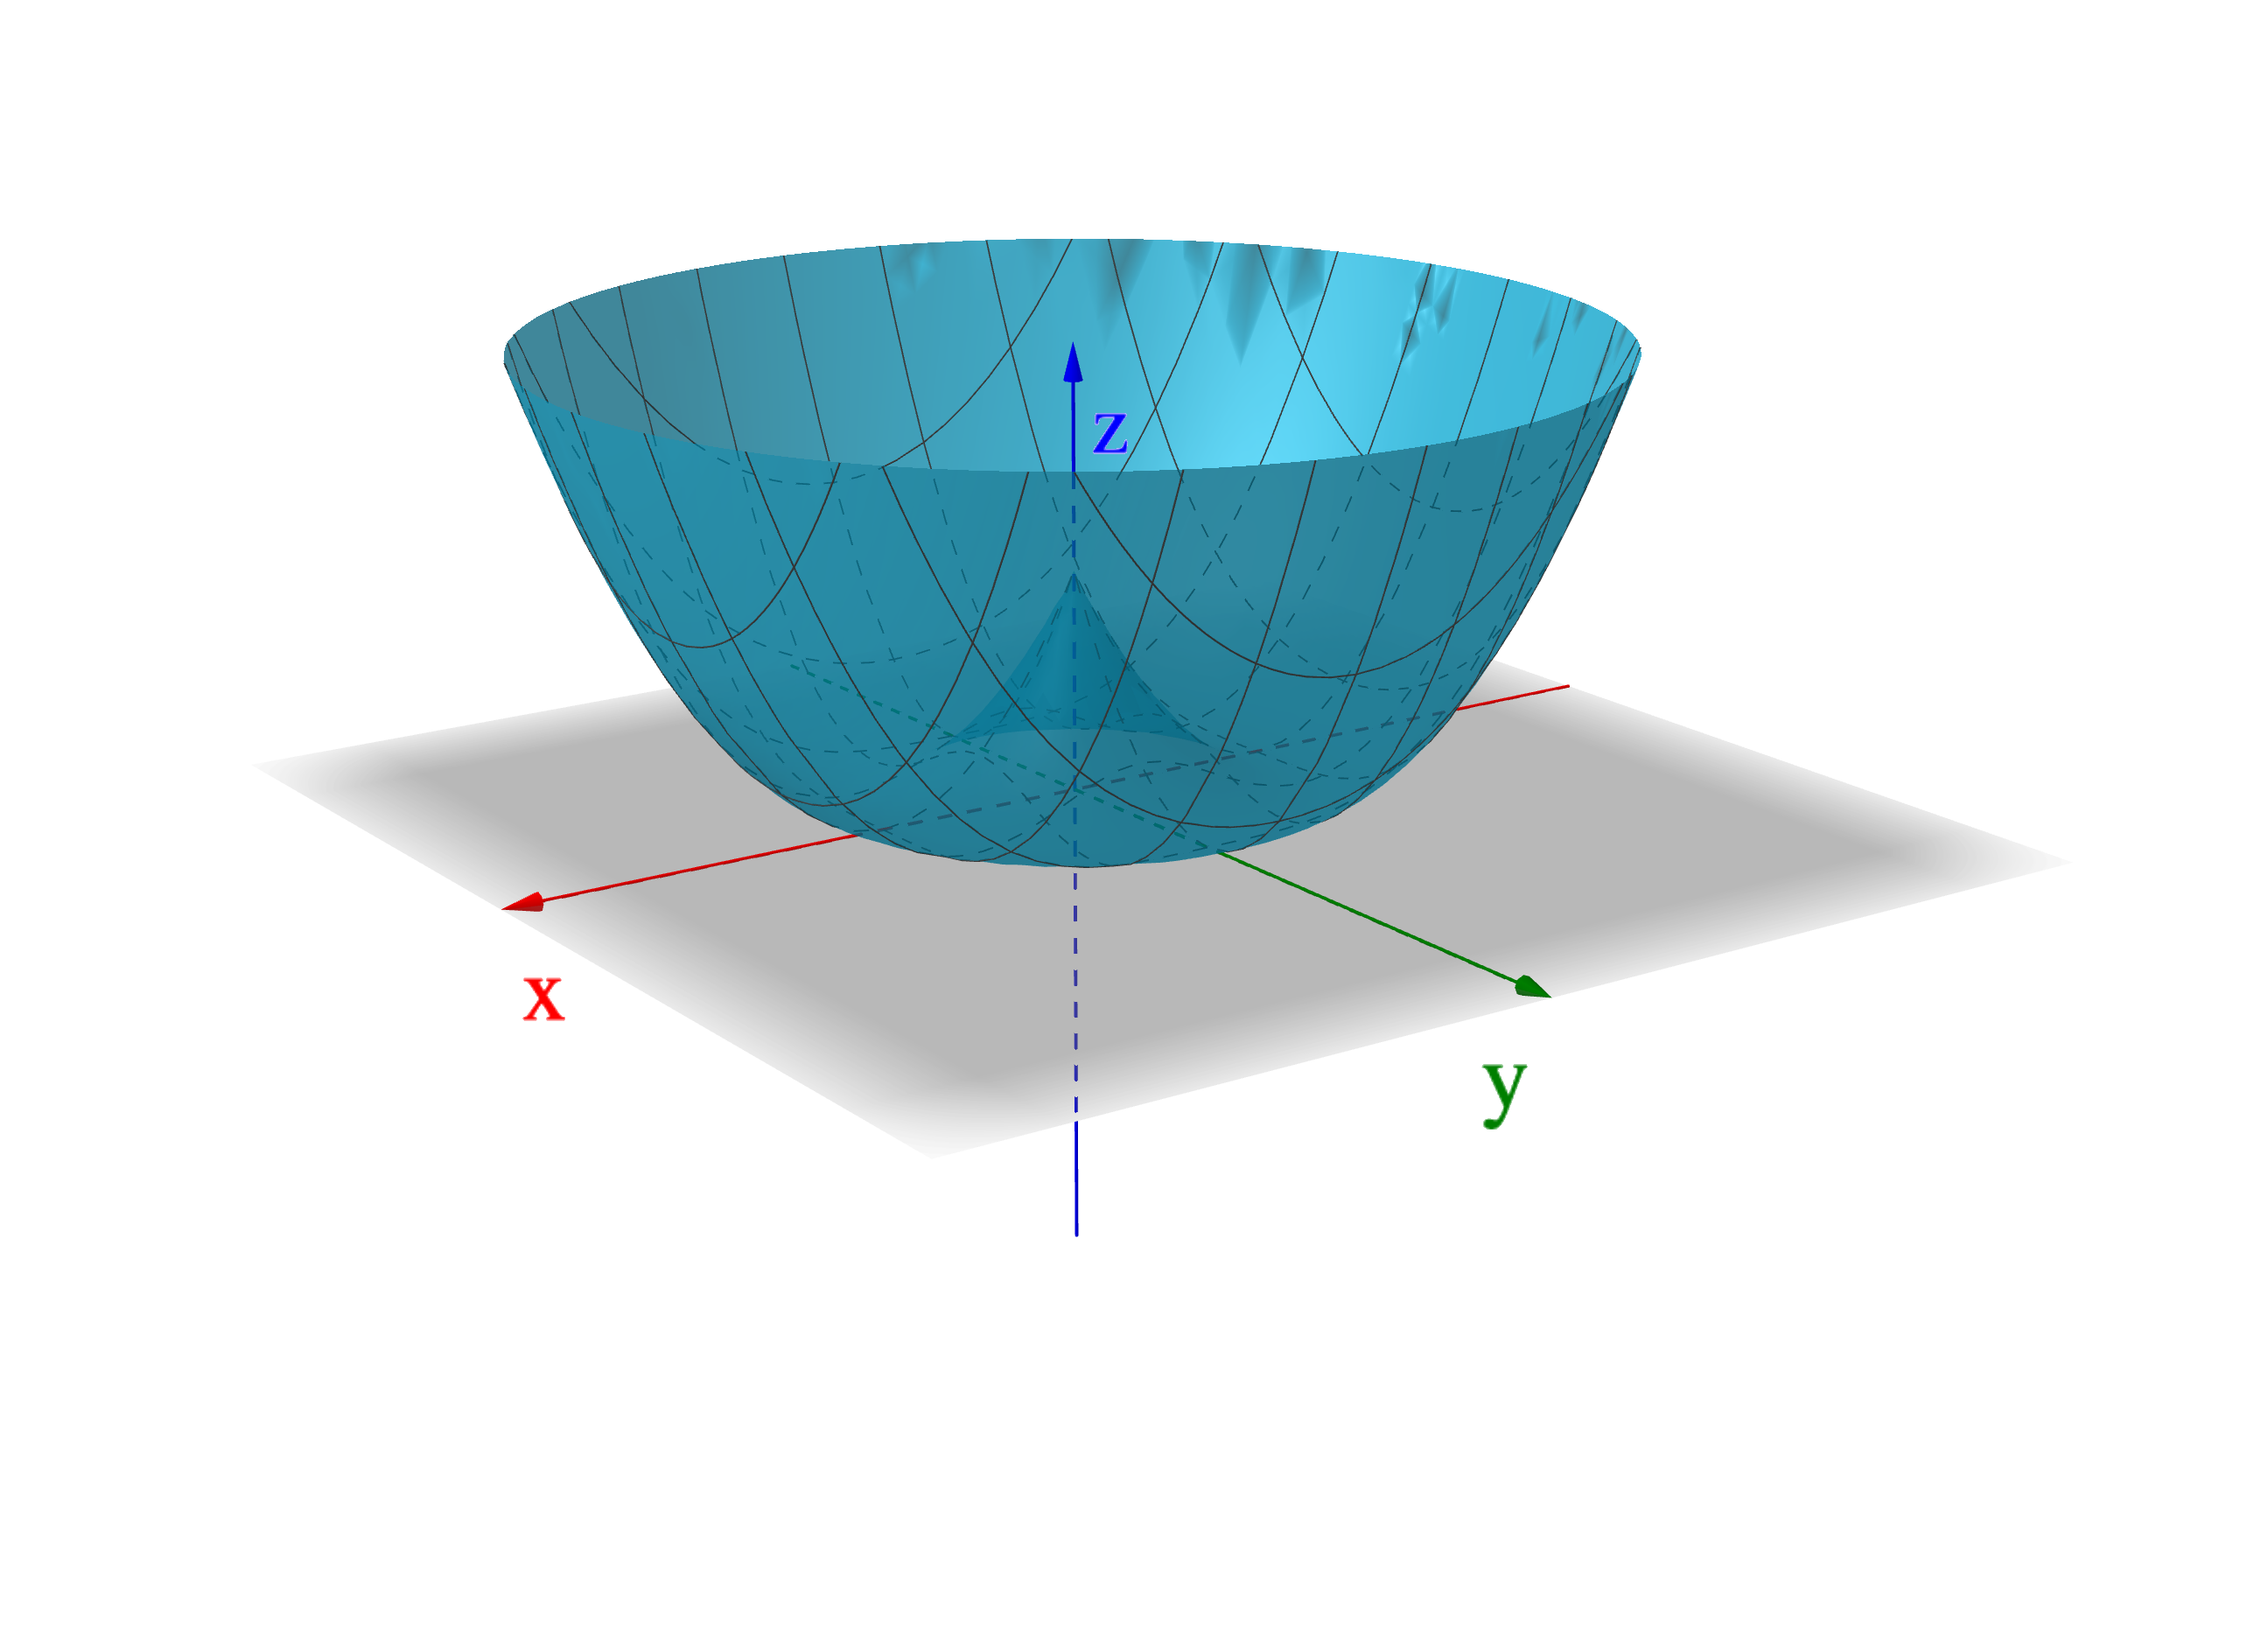
\includegraphics[width=0.9\linewidth]{Plots/e_1_2/5.png} \end{center}
    \end{minipage}

    \item
    \begin{minipage}[t]{0.25\linewidth}
        $\begin{aligned}[t]
            x^2 + y^2 + z^2    & = 2z \\
            r^2 + z^2 - 2z + 1 & = 1  \\
            r^2 + (z - 1)^2    & = 1
        \end{aligned}$
    \end{minipage}
    \begin{minipage}[c]{0.2\linewidth}
        \begin{center}
            \begin{tikzpicture}
                \draw[->] (-1.2, 0) -- (1.2, 0) node[right] {$r_{(y)}$};
                \draw[->] (0, -0.2) -- (0, 2.2) node[above] {$z$};

                \draw[thick,blue] (0,2) arc (90:-90:1cm and 1cm);

                \node[red] at (0,1) {$r^2 + (z - 1)^2 = 1$};
            \end{tikzpicture}
        \end{center}
    \end{minipage}
    \begin{minipage}[c]{0.5\linewidth}
        \begin{center} 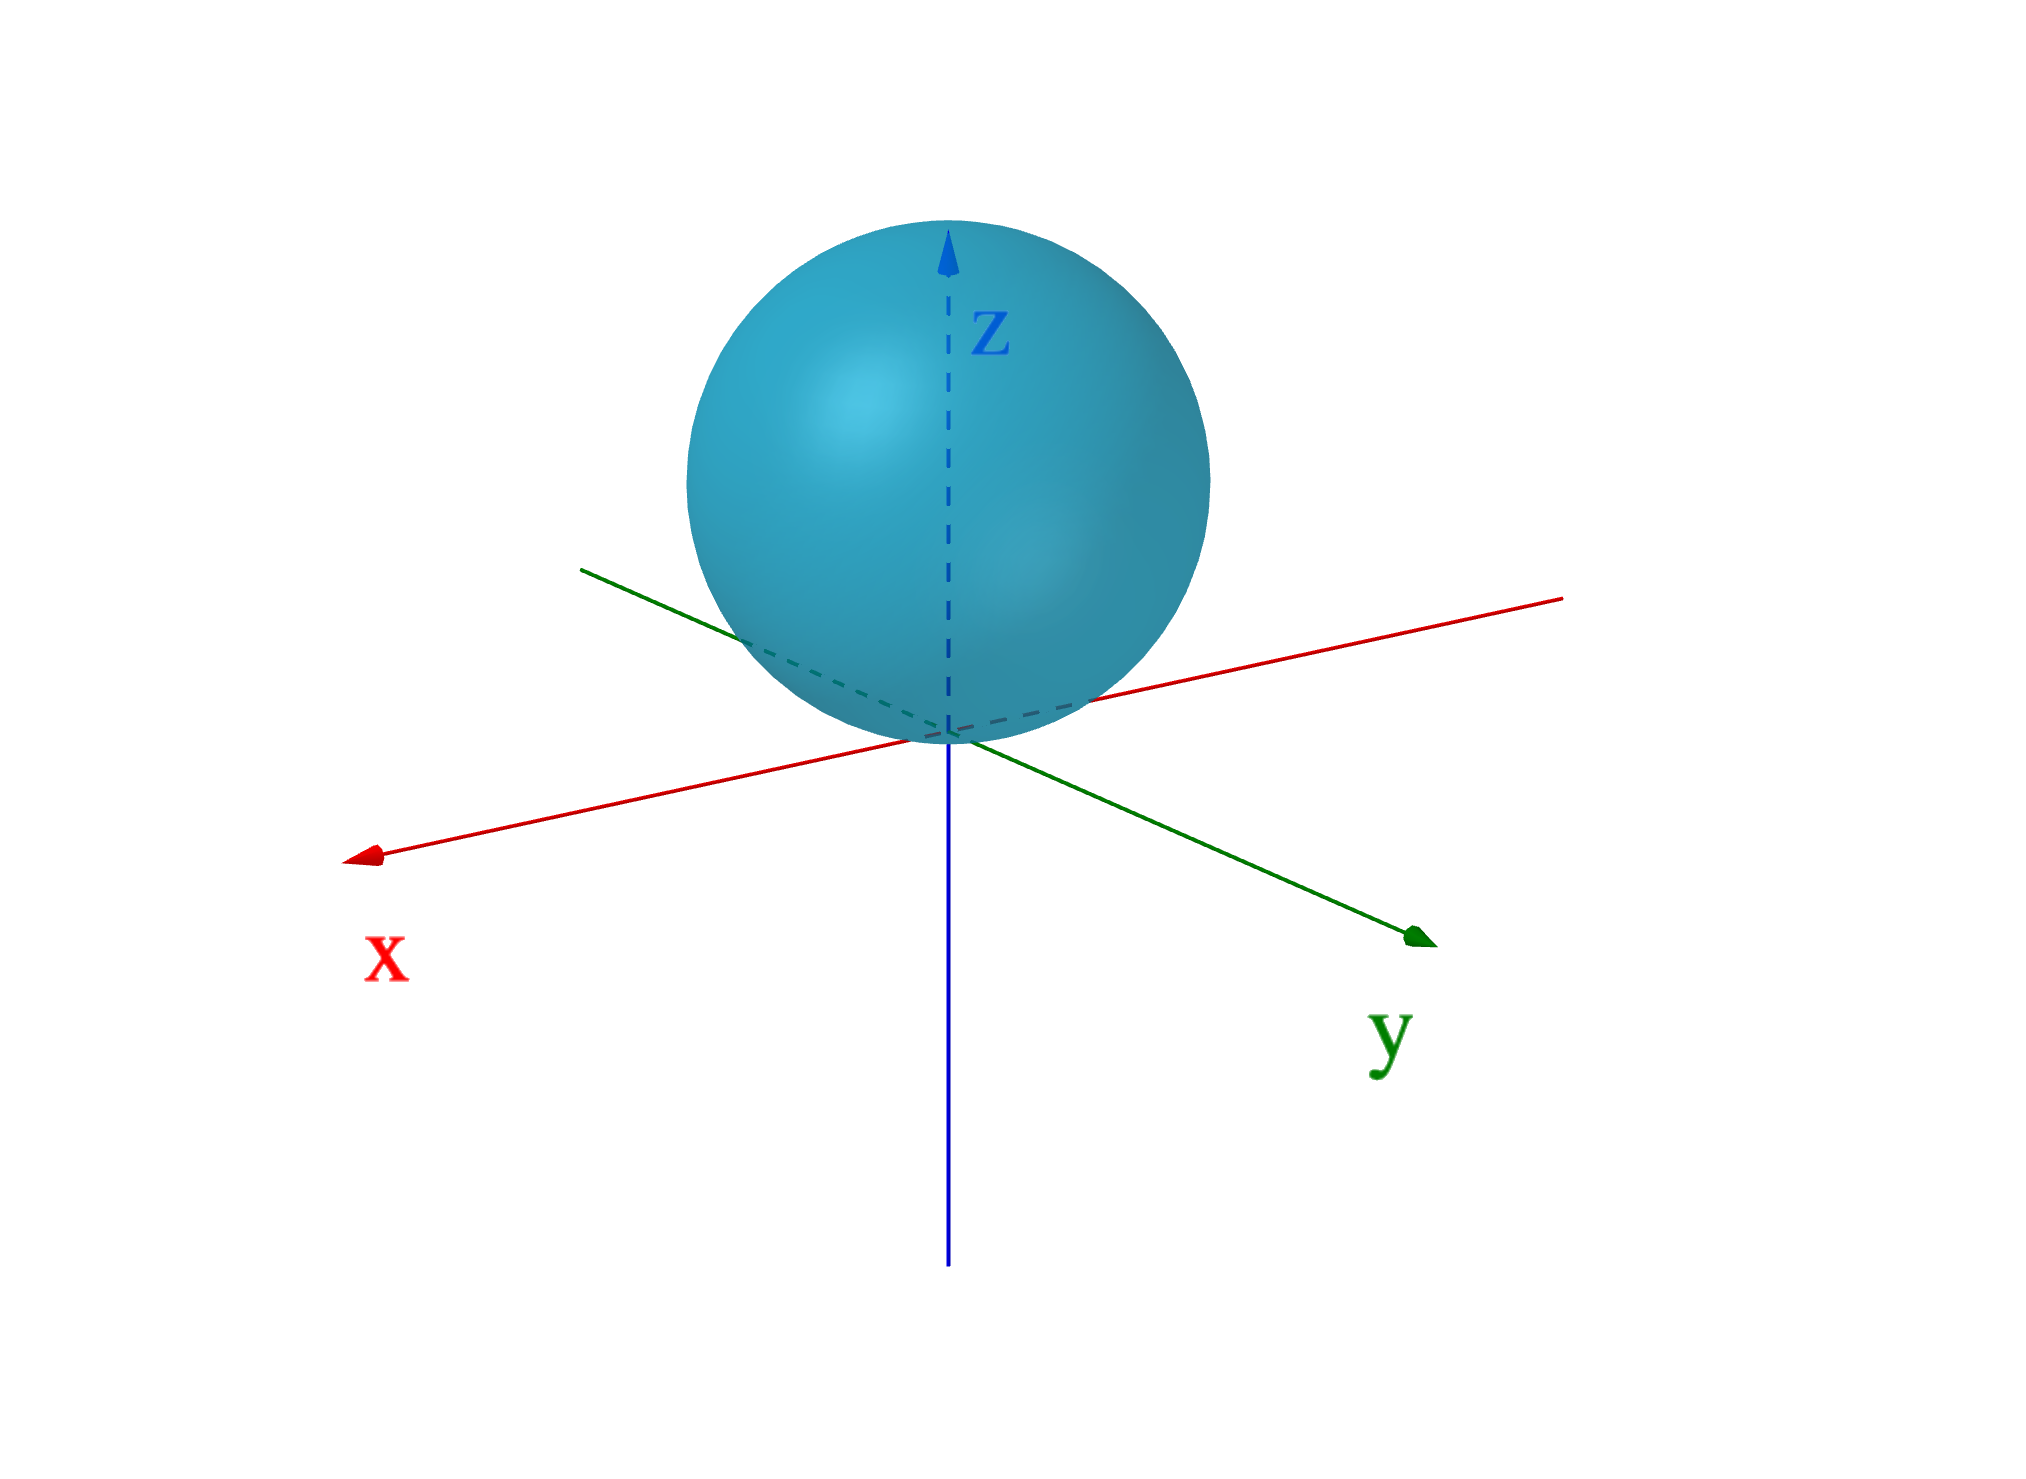
\includegraphics[width=0.9\linewidth]{Plots/e_1_2/6.png} \end{center}
    \end{minipage}
\end{enumerate}

\section*{Chapter 2}

\subsection*{Exercise 2.1}

\begin{enumerate}
    \item 
    $\begin{aligned}[t]
        \det \begin{pmatrix} 3 & -1 \\ 2 & 5 \end{pmatrix} 
        & = 3 \times 5 - 2 \times (-1) \\
        & = 15 + 2                     \\
        & = 17
    \end{aligned}$

    {~~~}

    \item 
    $\begin{aligned}[t]
        \det \begin{pmatrix} 1 & 3 & -3 \\ -3 & -5 & 2 \\ -4 & 4 & -6 \end{pmatrix}
        & = 1 \cdot \det \begin{pmatrix} -5 & 2 \\ 4 & -6 \end{pmatrix} - 3 \cdot \det \begin{pmatrix} -3 & 2 \\ -4 & -6 \end{pmatrix} + (-3) \cdot \det \begin{pmatrix} -3 & -5 \\ -4 & 4 \end{pmatrix} \\
        & = 1 \cdot 22 - 3 \cdot 26 + (-3) \cdot (-32)                  \\
        & = 22 - 78 + 96                                                \\
        & = 40
    \end{aligned}$

    {~~~}

    \item 
    $\begin{aligned}[t]
        \det \begin{pmatrix} 3 & 1 & 0 \\ 1 & 3 & 4 \\ 0 & 0 & 4 \end{pmatrix} & = 0 \cdot \det \begin{pmatrix} 1 & 0 \\ 3 & 4 \end{pmatrix} - 0 \cdot \det \begin{pmatrix} 3 & 0 \\ 1 & 4 \end{pmatrix} + 4 \cdot \det \begin{pmatrix} 3 & 1 \\ 1 & 3 \end{pmatrix}
        & \text{since }\begin{pmatrix} + & - & + \\ - & + & - \\ + & - & + \end{pmatrix}             \\
                                                                               & = 0 - 0 + 4 \cdot 8 \\
                                                                               & = 32
    \end{aligned}$
\end{enumerate}

\subsection*{Exercise 2.2}

\begin{minipage}[t]{0.45\linewidth}
    \begin{enumerate}
        \item 
        $\begin{aligned}[t]
            | \vec{a} |           & = \sqrt{\vec{a} \cdot \vec{a}}                          \\
                                  & = \sqrt{4^2 + 3^2}                                      \\
                                  & = 5
            \\ \\
            | \vec{b} |           & = \sqrt{\vec{b} \cdot \vec{b}}                          \\
                                  & = \sqrt{2^2 + (-1)^2}                                   \\
                                  & = \sqrt{5}
            \\ \\
            \vec{a} \cdot \vec{b} & = 4 \cdot 2 + 3 \cdot (-1)                              \\
                                  & = 5
            \\ \\
            \vec{a} \cdot \vec{b} & = | \vec{a} | | \vec{b} | \cos(\theta)                  \\
            \cos \theta           & = \frac{\vec{a} \cdot \vec{b}}{| \vec{a} | | \vec{b} |} \\
                                  & = \frac{5}{5 \cdot \sqrt{5}}                            \\
            \theta                & = \arccos \left( \frac{1}{\sqrt{5}} \right)
        \end{aligned}$
    \end{enumerate}
\end{minipage}
\begin{minipage}[t]{0.45\linewidth}
    \begin{enumerate} \setcounter{enumi}{1}
        \item 
        $\begin{aligned}[t]
            | \vec{a} |           & = \sqrt{\vec{a} \cdot \vec{a}}                          \\
                                  & = \sqrt{4^2 + 0^2 + 2^2}                                \\
                                  & = 2\sqrt{5}
            \\ \\
            | \vec{b} |           & = \sqrt{\vec{b} \cdot \vec{b}}                          \\
                                  & = \sqrt{2^2 + (-1)^2 + 0^2}                             \\
                                  & = \sqrt{5}
            \\ \\
            \vec{a} \cdot \vec{b} & = 4 \cdot 2 + 0 \cdot (-1) + 2 \cdot 0                  \\
                                  & = 8
            \\ \\
            \vec{a} \cdot \vec{b} & = | \vec{a} | | \vec{b} | \cos(\theta)                  \\
            \cos \theta           & = \frac{\vec{a} \cdot \vec{b}}{| \vec{a} | | \vec{b} |} \\
                                  & = \frac{8}{2\sqrt{5} \cdot \sqrt{5}}                    \\
            \theta                & = \arccos \left( \frac{4}{5} \right)
        \end{aligned}$
    \end{enumerate}
\end{minipage}

\vfill
\subsection*{Exercise 2.3}

$\begin{aligned}[t]
    \vec{x} \times \vec{y} 
    & = \det \begin{pmatrix} i & j & k \\ 3 & -2 & 1 \\ 1 & -1 & 1 \end{pmatrix} \\
    & = i \cdot \det \begin{pmatrix} -2 & 1 \\ -1 & 1 \end{pmatrix} - j \cdot \det \begin{pmatrix} 3 & 1 \\ 1 & 1 \end{pmatrix} + k \cdot \begin{pmatrix} 3 & -2 \\ 1 & -1 \end{pmatrix} \\
    & = (-1, -2, -1)
\end{aligned}$

\subsection*{Exercise 2.4}

\begin{enumerate}
    \item
    $\begin{aligned}[t]
        \vec{v} 
        & =(3, -2, 4) - (-8, 0, 4)                                                                   \\
        & = (11, -2, 0)
        \\
        \vec{r} 
        & = t\begin{bmatrix} 11 \\ 2 \\ 0 \end{bmatrix} + \begin{bmatrix} -8 \\ 0 \\ 4 \end{bmatrix}
    \end{aligned}$

    {~~~}

    \item
    $\begin{cases}
        \vec{r}_0 = (0, 0, 0) \\
        \vec{n} = (1, 5, 2)
    \end{cases}$

    {~~~}

    $\begin{aligned}[t]
        \vec{n} \cdot \vec{r}                                   
        & = \vec{n} \cdot \vec{r}_0                                                                   \\
        \begin{bmatrix} 1 \\ 5 \\ 2 \end{bmatrix} \cdot \vec{r} 
        & = \begin{bmatrix} 1 \\ 5 \\ 2 \end{bmatrix} \cdot \begin{bmatrix} 0 \\ 0 \\ 0 \end{bmatrix} \\
        \begin{bmatrix} 1 \\ 5 \\ 2 \end{bmatrix} \cdot \vec{r} 
        & = 0
    \end{aligned}$

    {~~~}

    \item
    $\begin{cases}
        \vec{r}_0 = (2, 4, 6) \\
        \vec{n} ~= (1, 1, -1)
    \end{cases}$

    {~~~}

    $\begin{aligned}[t]
        \vec{n} \cdot \vec{r}                                    
        & = \vec{n} \cdot \vec{r}_0                                                                     \\
        \begin{bmatrix} 1 \\ 1 \\ -1 \end{bmatrix} \cdot \vec{r} 
        & = \begin{bmatrix} 1 \\ 1 \\ -1 \end{bmatrix} \cdot \begin{bmatrix} 2 \\ 4 \\ -6 \end{bmatrix} \\
        \begin{bmatrix} 1 \\ 1 \\ -1 \end{bmatrix} \cdot \vec{r} & = 0
    \end{aligned}$

    {~~~}

    \item
    $\vec{x} = (1, 0, 1) - (0, 1, 1) = (1, -1, 0)$, and $\vec{y} = (1, 1, 0) - (0, 1, 1) = (1, 0, -1)$.

    {~~~}

    $\begin{aligned}[t]
        \vec{n}
        & = \vec{x} \times \vec{y}\\
        & = \det \begin{pmatrix} i & j & k \\ 1 & -1 & 0 \\ 1 & 0 & -1 \end{pmatrix} \\
        & = i \cdot \det \begin{pmatrix} -1 & 0 \\ 0 & -1 \end{pmatrix} - j \cdot \det \begin{pmatrix} 1 & 0 \\ 1 & -1 \end{pmatrix} + k \cdot \det \begin{pmatrix} 1 & -1 \\ 1 & 0 \end{pmatrix} \\
        & = \begin{bmatrix} 1 \\ 1 \\ 1 \end{bmatrix}
    \end{aligned}$

    $\begin{cases}
        \vec{r}_0 = (0, 1, 1) \\
        \vec{n} ~= (1, 1, 1)
    \end{cases}$

    {~~~}

    $\begin{aligned}[t]
        \vec{n} \cdot \vec{r}
        & = \vec{n} \cdot \vec{r}_0                                                                   \\
        \begin{bmatrix} 1 \\ 1 \\ 1 \end{bmatrix} \cdot \vec{r}
        & = \begin{bmatrix} 1 \\ 1 \\ 1 \end{bmatrix} \cdot \begin{bmatrix} 0 \\ 1 \\ 1 \end{bmatrix} \\
        \begin{bmatrix} 1 \\ 1 \\ 1 \end{bmatrix} \cdot \vec{r}
        & = 0
    \end{aligned}$

    {~~~}

    \item 
    $\begin{aligned}[t]
        \vec{r}_0 & = \frac{(3, 1, 5) + (-2, 0, 0)}{2} \\
                  & = \frac{1}{2} (1, 1, 5)
        \\ \\
        \vec{n}   & = (-2, 0, 0) - (3, 1, 5)           \\
                  & = (-5, -1, -5)
    \end{aligned}$

    {~~~}

    {~~~}

    $\begin{aligned}[t]
        \vec{n} \cdot \vec{r}     & = \vec{n} \cdot \vec{r}_0                \\
        (-5, 1, -5) \cdot \vec{r} & = (-5, 1, -5) \cdot \frac{1}{2}(1, 1, 5) \\
        -5x - y - 5z              & = \frac{1}{2}(-5 + 1 - 25)               \\
                                  & = \frac{-31}{2}
    \end{aligned}$
\end{enumerate}

\section*{Chapter 3}

\subsection*{Exercise 3.1}

\begin{enumerate}
    \item 
    \begin{minipage}[t]{0.45\linewidth}
        At $k = 2$, 
        $\begin{aligned}[t]
            4x^2 + y^2 + 1 &= 2 \\
            4x^2 + y^2     &= 1 \\
            \left(\frac{x}{\frac{1}{2}}\right)^2 + \left(\frac{y}{1}\right)^2 &= 1
        \end{aligned}$
    \end{minipage}
    \begin{minipage}[t]{0.45\linewidth}
        At $k = 5$, 
        $\begin{aligned}[t]
            4x^2 + y^2 + 1      &= 5 \\
            4x^2 + y^2          &= 4 \\
            x^2 + \frac{y^2}{4} &= 1 \\
            \left(\frac{x}{1}\right)^2 + \left(\frac{y}{2}\right)^2 &= 1
        \end{aligned}$
    \end{minipage}

    \begin{center}
        \tikzsetnextfilename{c03e01-01}%
        \begin{tikzpicture}
            \draw[->] (-2.2,0) -- (2.2,0) node[right] {$x$};
            \draw[->] (0,-2.7) -- (0,2.7) node[above] {$y$};
            
            \draw[thick,blue] (0,0) ellipse (0.5cm and 1cm);
            \draw[thick,DarkGreen] (0,0) ellipse (1cm and 2cm);

            \draw[thick,red] (0.5,0.25) -- (0.5,0) node[below left] {$\frac{1}{2}$};
            \draw[thick,red] (1,0.25) -- (1,0) node[below left] {$1$};

            \draw[thick,red] (0.25,1) -- (0,1) node[left] {$1$};
            \draw[thick,red] (0.25,2) -- (0,2) node[left] {$2$};

            \node[blue] at (1.5,3) {Level set at $k = 2$};
            \node[DarkGreen] at (1.5,2.5) {Level set at $k = 5$};
        \end{tikzpicture}
    \end{center}

    \item 
    \begin{minipage}[t]{0.45\linewidth}
        At $k = 0$, 
        $\begin{aligned}[t]
            x^2 + y^2 - z &= 0 \\
            x^2 + y^2     &= z \\
            r^2           &= z
        \end{aligned}$
        
        \begin{center} 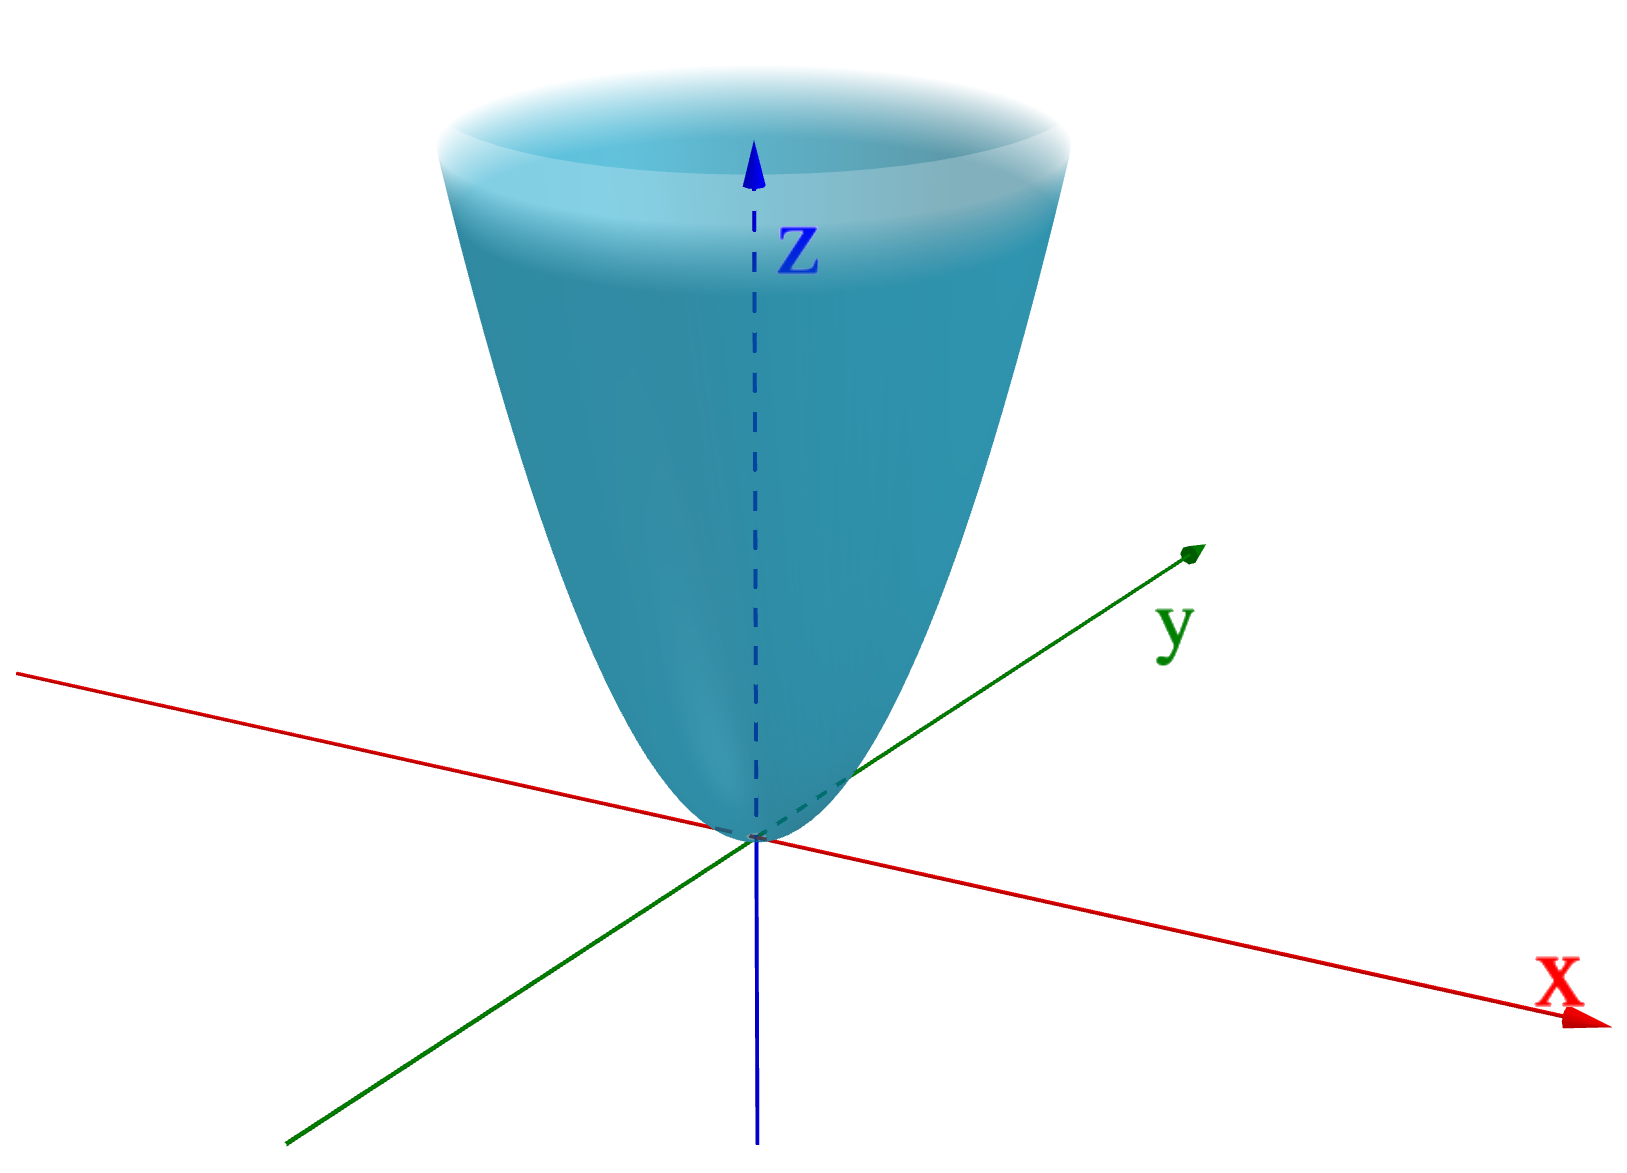
\includegraphics[width=\linewidth]{Plots/e_1_7/1.png} \end{center}
    \end{minipage}
    \begin{minipage}[t]{0.45\linewidth}
        At $k = 2$, 
        $\begin{aligned}[t]
            x^2 + y^2 - z &= 2 \\
            x^2 + y^2 - 2 &= z \\
            r^2 - 2       &= z
        \end{aligned}$

        \begin{center} 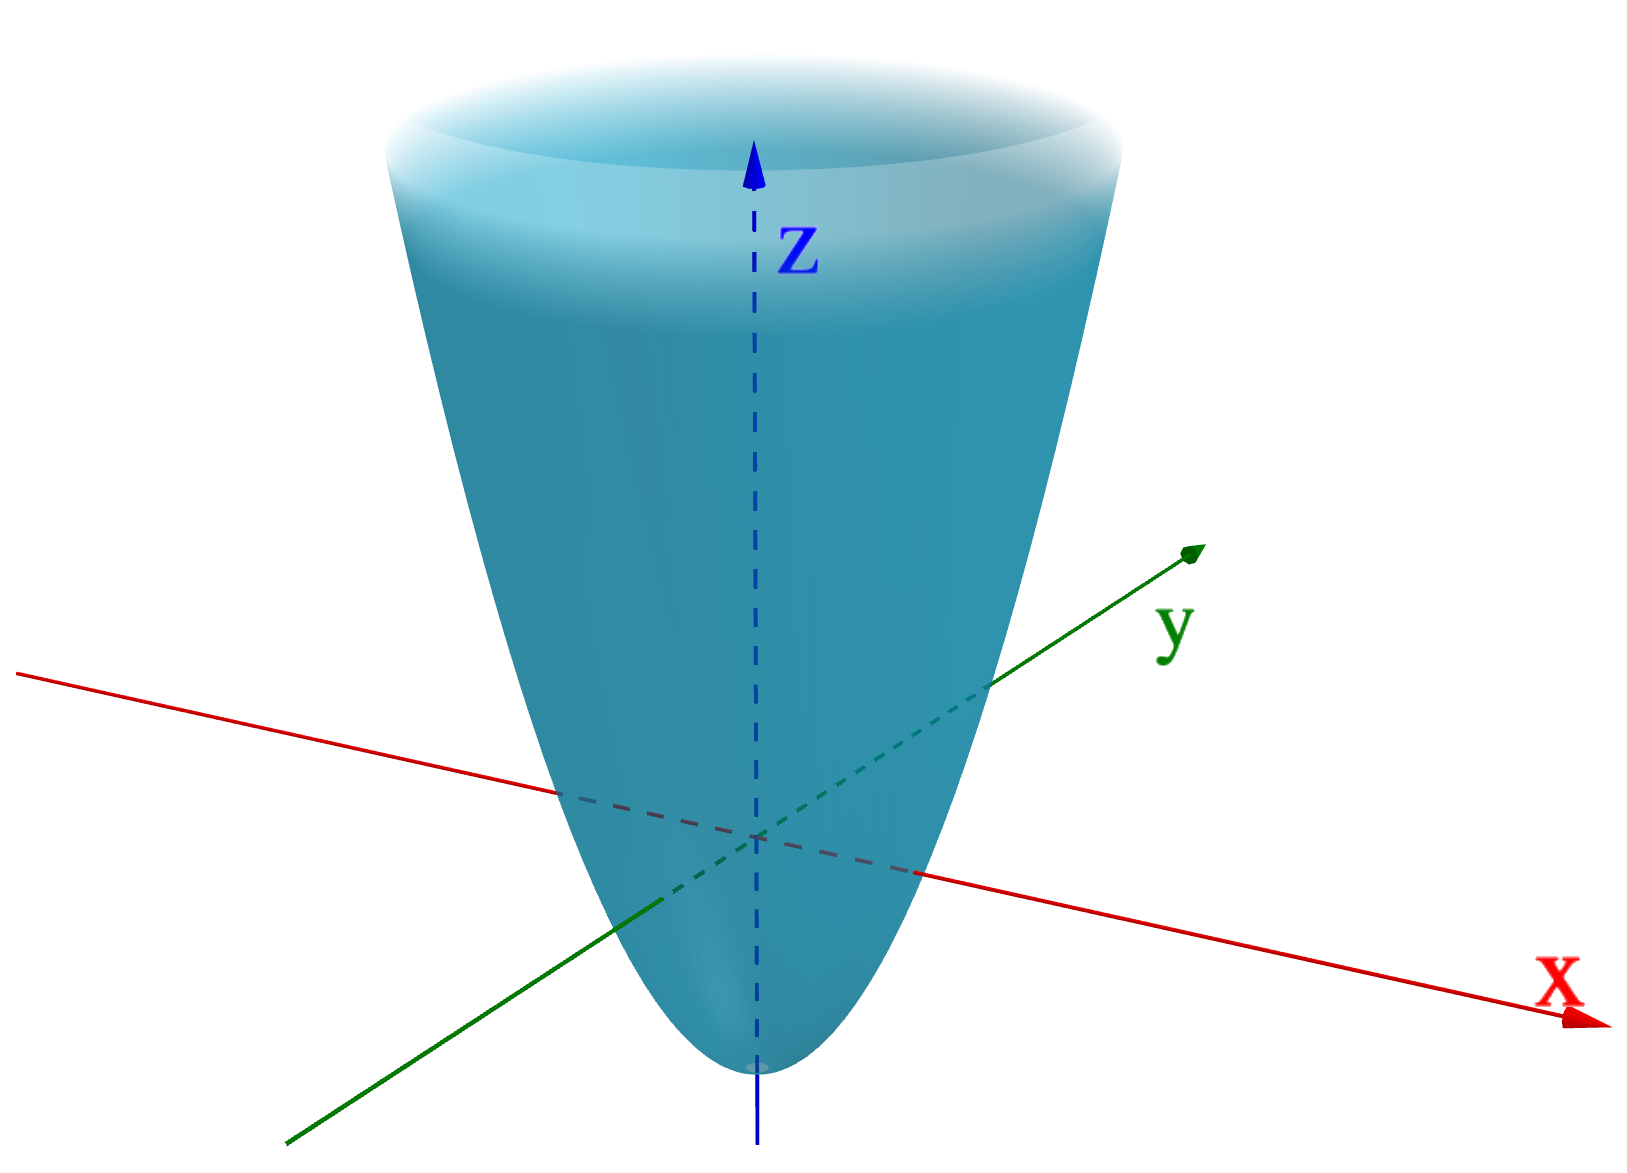
\includegraphics[width=\linewidth]{Plots/e_1_7/2.png} \end{center}
    \end{minipage}
\end{enumerate}

\subsection*{Exercise 3.2}

\begin{itemize}
        \item For $x = 0$, $\lim_{(x,y)\to(0,0)}f(x,y) = \lim_{y\to0}\frac{0}{0 + y^2} = 0$. 

        {~~~}

        \item For $y = x$, $\lim_{(x,y)\to(0,0)}f(x,y) = \lim_{x\to0} \frac{x^2x}{x^4 + x^2} = \lim_{x\to0} \frac{x}{x+1} = 0$. 

        {~~~}

        \item For $y = 0$, $\lim_{(x,y)\to(0,0)}f(x,y) = \lim_{x\to0}\frac{0}{x^4 + 0} = 0$. 

        {~~~}

        \item For $y = x^2$, $\lim_{(x,y)\to(0,0)}f(x,y) = \lim_{x\to0} \frac{x^2x^2}{x^4 + (x^2)^2} = \lim_{x\to0} \frac{x^4}{2x^4} = \frac{1}{2}$. 
\end{itemize} 

Thus, the limit at $(a,y) = (0,0)$ does not exist. 

\subsection*{Exercise 3.3}

$$|f(x, y)| = \left| \frac{xy}{\sqrt{x^4 + y^2}} \right| \le \left| \frac{xy}{\sqrt{y^2}} \right| = \left| \frac{xy}{y} \right| = |x| \to 0$$

Thus, by the Squeeze Theorem, $\lim_{(x,y) \to (0,0)} \frac{xy}{\sqrt{x^4 + y^2}} = 0 = f(0, 0)$. 

Thus, the function is continuous at $(0, 0)$. 

\subsection*{Exercise 3.4}

By removing $2x^4$ from the denominator, we obtain $\left| \frac{x^2 \sin^2{y}}{2x^4 + y^2} \right| \le \left| \frac{x^2 \sin^2{y}}{y^2} \right|$. 

{~~~}

Note that $| \sin{\theta} | \le | \theta |$, and that as $\theta \to 0$, $\sin \theta \approx \theta$. This is the \term{small angle approximation}. 

\begin{center}
    \tikzsetnextfilename{c03e04-01}%
    \begin{tikzpicture}
        \draw[->] (-2.6, 0) -- (2.6, 0) node[right] {$x$};
        \draw[->] (0, -2.2) -- (0, 1.7) node[above] {$y$};

        \draw[thick,blue,domain=-2.5:2.5,smooth] plot (\x, {sin(2*\x r)}) node[below left] {$y = \sin{x}$};
        \draw[thick,DarkGreen,domain=-1:1] plot (\x, {2*\x}) node[right] {$y = x$};
    \end{tikzpicture}
\end{center}

So $\left| \frac{x^2 \sin^2{y}}{y^2} \right| \approx \left| \frac{x^2 \cdot y^2}{y^2} \right| = \left| x^2 \right| \to 0$. 

{~~~}

Then, by the Squeeze Theorem, $\lim_{(x,y) \to (0,0)} \frac{x^2 \sin^2{y}}{2x^4 + y^2} = 0$. 

\subsection*{Exercise 3.5}

\begin{enumerate}
    \item 
    $\frac{\partial f}{\partial x} = 2x(y + 1)$ and 
    $\frac{\partial f}{\partial y} = x^2 - 1$. 
    
    So $\nabla f = \left( \frac{\partial f}{\partial x}, \frac{\partial f}{\partial y} \right) = (2x(y + 1), x^2 - 1)$. 

    {~~~}

    \item 
    $\frac{\partial f}{\partial x} = 2{\color{red}y}(xy - 2)$ and 
    $\frac{\partial f}{\partial y} = 2{\color{red}x}(xy - 2)$. 
    
    So $\nabla f = \left( \frac{\partial f}{\partial x}, \frac{\partial f}{\partial y} \right) = (2y(xy - 2), 2x(xy - 2))$. 

    {~~~}

    \item 
    $\frac{\partial f}{\partial x} = \frac{-2}{(x + 3y)^2}$ and 
    $\frac{\partial f}{\partial y} = \frac{-6}{(x + 3y)^2}$. 
    
    So $\nabla f = \left( \frac{\partial f}{\partial x}, \frac{\partial f}{\partial y} \right) = \left( \frac{-2}{(x + 3y)^2}, \frac{-6}{(x + 3y)^2} \right)$. 

    {~~~}

    \item 
    $\frac{\partial f}{\partial x} = e^{x + 4y}$ and 
    $\frac{\partial f}{\partial y} = 4e^{x + 4y}$. 
    
    So $\nabla f = \left( \frac{\partial f}{\partial x}, \frac{\partial f}{\partial y} \right) = (e^{x + 4y}, 4e^{x + 4y})$. 

    {~~~}

    \item 
    $\frac{\partial f}{\partial x} = 2x$, 
    $\frac{\partial f}{\partial y} = 0$, and
    $\frac{\partial f}{\partial z} = 2$. 
    
    So $\nabla f = \left( \frac{\partial f}{\partial x}, \frac{\partial f}{\partial y}, \frac{\partial f}{\partial z} \right) = (2x, 0, 2)$. 

    {~~~}

    \item 
    $\frac{\partial f}{\partial x} = y{\color{red}z}e^{xz}$, 
    $\frac{\partial f}{\partial y} = e^{xy}$, and
    $\frac{\partial f}{\partial z} = {\color{red}x}ye^{xz}$. 
    
    So $\nabla f = \left( \frac{\partial f}{\partial x}, \frac{\partial f}{\partial y}, \frac{\partial f}{\partial z} \right) = (yze^{xz}, e^{xz}, xye^{xz})$. 
\end{enumerate}

\subsection*{Exercise 3.6}

\begin{minipage}[t]{0.3\linewidth}
    $\begin{aligned}[t]
        \vec{u} & = \frac{\vec{v}}{| \vec{v} |}                             \\
                & = \frac{(1, 3)}{\sqrt{1^2 + 3^2}}                         \\
                & = \frac{1}{\sqrt{10}}\begin{bmatrix} 1 \\ 3 \end{bmatrix}
    \end{aligned}$
\end{minipage}
\begin{minipage}[t]{0.3\linewidth}
    $\begin{aligned}[t]
        \nabla f 
        & = \left( \frac{\partial f}{\partial x}, \frac{\partial f}{\partial y} \right) \\
        & = \begin{bmatrix} 2ye^{2x} \\ e^{2x} + 2y \end{bmatrix} \\
        \nabla f(0, 0) 
        & = \begin{bmatrix}
            2 \cdot 0 \cdot e^{2 \cdot 0} \\
            e^{2 \cdot 0} + 2 \cdot 0
        \end{bmatrix} \\
        &= \begin{bmatrix} 0 \\ 1 \end{bmatrix}
    \end{aligned}$

\end{minipage}
\begin{minipage}[t]{0.3\linewidth}
    So $\begin{aligned}[t]
        D_{\vec{u}} f 
        & = \nabla f \cdot \vec{u} \\
        & = \begin{bmatrix} 0 \\ 1 \end{bmatrix} \cdot \frac{1}{\sqrt{10}} \begin{bmatrix} 1 \\ 3 \end{bmatrix} \\
        & = \frac{3}{\sqrt{10}}
    \end{aligned}$
\end{minipage}

\subsection*{Exercise 3.7}

$\nabla f = \left( \frac{\partial f}{\partial x}, \frac{\partial f}{\partial y}, \frac{\partial f}{\partial z} \right) = \begin{bmatrix} 2xy \\ x^2 \\ 1 \end{bmatrix}$. 

The directional vector, $\nabla f(2, 2, 1) = \begin{bmatrix} 2 \cdot 2 \cdot 2 \\ 2^2 \\ 1 \end{bmatrix} = \begin{bmatrix} 8 \\ 4 \\ 1 \end{bmatrix}$. 

The maximum rate of change is $| \nabla f(2, 2, 1) | = \sqrt{8^2 + 4^2 + 1} = 9$. 

Thus, the maximum rate of change at $(2, 2, 1)$ is $9$ in the $\begin{bmatrix} 8 \\ 4 \\ 1 \end{bmatrix}$ direction. 

\subsection*{Exercise 3.8}

$\nabla f  = \left( \frac{\partial f}{\partial x} \\ \frac{\partial f}{\partial y} \\ \frac{\partial f}{\partial z} \right) = \left( y^2e^z, 2xye^z, xy^2e^z \right)$

So $\vec{n} = \nabla f(1,1,1) = \begin{bmatrix} 1^2 \cdot e^1 \\ 2 \cdot 1 \cdot 1 \cdot e^1 \\ 1 \cdot 1^2 \cdot e^1 \end{bmatrix} = \begin{bmatrix} e \\ 2e \\ e \end{bmatrix}$.

$\begin{aligned}[t]
    \text{For the equation of the tangent plane, }
    \vec{n} \cdot \vec{r}
     & = \vec{n} \cdot \vec{r}_0                                                                    \\
    \begin{bmatrix} e \\ 2e \\ e \end{bmatrix} \cdot \vec{r}
     & = \begin{bmatrix} e \\ 2e \\ e \end{bmatrix} \cdot \begin{bmatrix} 1 \\ 1 \\ 1 \end{bmatrix} \\
    ex + 2ey + ez
     & = e + 2e + e                                                                                 \\
     & = 4e                                                                                         \\
    x + 2y + z
     & = 4
\end{aligned}$

\subsection*{Exercise 3.9}

\begin{enumerate}[label=\alph*)]
    \item Let $\vec{u} = (a,b)$ such that $a^2 + b^2 = 0$ (that is, $\vec{u}$ is a unit vector). 
    
    We focus on $\vec{a} = (0,0)$. 

    {~~~}

    Now, $\begin{aligned}[t]
        D_{\vec{u}} f(\vec{a}) & = \lim_{h\to0} \frac{f(\vec{a} + h\vec{u}) - f(\vec{a})}{h}          \\
                               & = \lim_{h\to0} \frac{f(ha,hb) - f(0,0)}{h}                           \\
                               & = \lim_{h\to0} \frac{1}{h} \cdot \frac{ha \cdot hb}{(ha)^2 + (hb)^2} \\
                               & = \lim_{h\to0} \frac{1}{h} \cdot \frac{h^2ab}{h^2(a^2 + b^2)}        \\
                               & = \lim_{h\to0} \frac{ab}{h}                                          \\
                               & = \begin{cases}
                                        0          & b = 0 ~ (\vec{u} = (1,0))\\
                                        0          & a = 0 ~ (\vec{u} = (0,1))\\
                                        \text{DNE} & \text{otherwise}
                                   \end{cases}
    \end{aligned}$

    {~~~}

    To check for continuity, we want $\lim_{(x,y)\to(0,0)} f(x,y) = f(0,0) = 0$. 

    \begin{itemize}
        \item For $x = 0$, $\lim_{(x,y)\to(0,0)} f(x,y) = \lim_{x\to0} \frac{0 \cdot y}{0^2 + y^2} = 0$.
        \item For $y = 0$, $\lim_{(x,y)\to(0,0)} f(x,y) = \lim_{y\to0} \frac{x \cdot 0}{x^2 + 0^2} = 0$.
        \item For $y = x$, $\lim_{(x,y)\to(0,0)} f(x,y) = \lim_{x\to0} \frac{x \cdot x}{x^2 + x^2} = \frac{1}{2} \neq 0$. 
    \end{itemize}

    {~~~}
    
    Thus, this function is not continuous. 

    {~~~}

    \item Let $\vec{u} = (a,b)$ such that $a^2 + b^2 = 0$ (that is, $\vec{u}$ is a unit vector). 
    
    We focus on $\vec{a} = (0,0)$. 

    {~~~}

    Now, $\begin{aligned}[t]
        D_{\vec{u}} f(\vec{a}) & = \lim_{h\to0} \frac{f(\vec{a} + h\vec{u}) - f(\vec{a})}{h} \\
                               & = \lim_{h\to0} \frac{f(ha,hb) - f(0,0)}{h}                  \\
                               & = \lim_{h\to0} \frac{1}{h} \cdot \sqrt{| ha \cdot hb |}     \\
                               & = \lim_{h\to0} \frac{1}{h} \cdot \sqrt{h^2 | a \cdot b |}   \\
                               & = \frac{|h|}{h} \sqrt{| a \cdot b |}                        \\
                               & = \begin{cases}
                                       0          & b = 0 ~ (\vec{u} = (1,0)) \\
                                       0          & a = 0 ~ (\vec{u} = (0,1)) \\
                                       \text{DNE} & \text{otherwise}
                                   \end{cases}
        \end{aligned}$

        {~~~}

        Since there is no division by $0$, this function is continuous. 
\end{enumerate}

\subsection*{Exercise 3.10}

\subsubsection*{Solution 1}

Let $\vec{u} = (a,b)$. 

We focus on $\vec{a} = (0,0)$. 

Now, 
$\begin{aligned}[t]
    D_{\vec{u}} f(\vec{a}) & = \lim_{h\to0} \frac{f(\vec{a} + h\vec{u}) - \cancelto{0}{f(\vec{a}})}{h} \\
                           & = \lim_{h\to0} \frac{f(ha, hb)}{h}                                        \\
                           & = \lim_{h\to0} \frac{1}{h} \cdot \frac{(ha)^2 \cdot hb}{(ha)^4 + (hb)^2}  \\
                           & = \lim_{h\to0} \frac{1}{h} \cdot \frac{h^3 \cdot ab}{h^2(h^2a^4 + b^2)}   \\
                           & = \lim_{h\to0} \frac{a^2b}{h^2a^4 + b^2}                                  \\
                           & = \begin{cases}
                                   0             & b = 0 ~ (\vec{u} = (1,0)) \\
                                   \frac{a^2}{b} & \text{otherwise}
                               \end{cases}
\end{aligned}$

Thus, the directional derivatives exist at $(0,0)$. 

{~~~}

For $f$ to be differentiable, we need $\lim_{\vec{h}\to\vec{0}} \frac{f(\vec{a} + \vec{h}) - f(\vec{a}) - \nabla f(\vec{a}) \cdot \vec{h}}{| \vec{h} |} = 0$. 

Note that $\nabla f(\vec{a}) = \left( \frac{\partial f}{\partial x}, \frac{\partial f}{\partial y} \right) = \begin{bmatrix} D_{(1,0)} f(\vec{a}) \\ D_{(0,1)} f(\vec{a}) \end{bmatrix} = \begin{bmatrix} 0 \\ 0 \end{bmatrix}$.

Let $(x,y) = \vec{x} = \vec{a} + \vec{h} = \vec{h}$ since $\vec{a} = (0,0)$. 

Thus, 
$\begin{aligned}[t]
    \lim_{\vec{h}\to\vec{0}} \frac{f(\vec{a} + \vec{h}) - \cancelto{0}{f(\vec{a})} - \cancelto{0}{\nabla f(\vec{a})} \cdot \vec{h}}{| \vec{h} |}
     & = \lim_{\vec{h}\to\vec{0}} \frac{f(\vec{a} + \vec{h})}{| \vec{h} |}          \\
     & = \lim_{(x,y)\to(0,0)} \frac{f(x,y)}{\sqrt{x^2 + y^2}}                       \\
     & = \lim_{(x,y)\to(0,0)} \frac{1}{\sqrt{x^2+y^2}} \cdot \frac{x^2y}{x^4 + y^2} 
\end{aligned}$

\begin{itemize}
    \item For $x = 0$, $\lim_{(x,y)\to(0,0)} \frac{1}{\sqrt{x^2+y^2}} \cdot \frac{x^2y}{x^4 + y^2} = \lim_{y\to0} \frac{1}{\sqrt{0^2+y^2}} \cdot \frac{0^2 \cdot y}{0^4 + y^2} = 0$. 
    \item For $y = 0$, $\lim_{(x,y)\to(0,0)} \frac{1}{\sqrt{x^2+y^2}} \cdot \frac{x^2y}{x^4 + y^2} = \lim_{x\to0} \frac{1}{\sqrt{x^2+0^2}} \cdot \frac{x^2 \cdot 0}{x^4 + 0^2} = 0$. 
    \item For $y = x$, $\begin{aligned}[t]
        \lim_{\vec{h}\to\vec{0}} \frac{f(\vec{a} + \vec{h}) - \cancelto{0}{f(\vec{a})} - \cancelto{0}{\nabla f(\vec{a})} \cdot \vec{h}}{| \vec{h} |}
         & = \lim_{(x,y)\to(0,0)} \frac{1}{\sqrt{x^2+y^2}} \cdot \frac{x^2y}{x^4 + y^2}                   \\
         & = \lim_{x\to0} \frac{1}{\sqrt{x^2 + x^2}} \cdot \frac{x^2 \cdot x}{x^4 + x^2}                  \\
         & = \lim_{x\to0} \frac{1}{\sqrt{2x^2}} \cdot \frac{\cancel{x^2} \cdot x}{\cancel{x^2} (x^2 + 1)} \\
         & = \lim_{x\to0} \frac{x}{\sqrt{2}|x|} \cdot \frac{1}{x^2 + 1}                                   \\
         & = \pm \frac{1}{\sqrt{2}}
    \end{aligned}$
\end{itemize}

Thus, $\lim_{\vec{h}\to\vec{0}} \frac{f(\vec{a} + \vec{h}) - f(\vec{a}) - \nabla f(\vec{a}) \cdot \vec{h}}{| \vec{h} |}$ does not exist. $f$ is not differentiable. 

\begin{center} \line(1,0) {250} \end{center}

\subsubsection*{Solution 2}

Take $\vec{a} = (0,0)$ and $\vec{u} = (a,b)$ \footnote{Here $\vec{u}$ is a always unit vector, so we have $a^2 + b^2 = 1$. },
$\begin{aligned}[t]
    D_{\vec{u}} f(\vec{a}) & = \lim_{h\to0} \frac{f(\vec{a} + h\vec{u}) - \cancelto{0}{f(\vec{a}})}{h} \\
                           & = \lim_{h\to0} \frac{f(ha, hb)}{h}                                        \\
                           & = \lim_{h\to0} \frac{1}{h} \cdot \frac{(ha)^2 \cdot hb}{(ha)^4 + (hb)^2}  \\
                           & = \lim_{h\to0} \frac{1}{h} \cdot \frac{h^3 \cdot ab}{h^2(h^2a^4 + b^2)}   \\
                           & = \lim_{h\to0} \frac{a^2b}{h^2a^4 + b^2}                                  \\
                           & = \begin{cases}
                                   0             & b = 0 ~ (\vec{u} = (1,0)) \\
                                   \frac{a^2}{b} & \text{otherwise}
                               \end{cases}
\end{aligned}$

Assume $f$ is differentiable at $(0,0)$. Then, $D_{\vec{u}}f = \nabla f \cdot \vec{u}$. 

Let $\vec{u} = (a,b)$, $\nabla f(\vec{a}) = (c,d)$. 
\begin{itemize}
    \item When $a = 1$, $b = 0$,  $D_{\vec{u}} f = 0$, and $\nabla f \cdot \vec{u} = (c, d) \cdot (1, 0) = c$. Thus, $c = 0$. 
    \item When $a = 0$, $b = 1$,  $D_{\vec{u}} f = a|b| = 0 \cdot 1 = 0$, and $\nabla f \cdot \vec{u} = (c, d) \cdot (0, 1) = d$. Thus, $d = 0$. 
    \item When $a = \frac{1}{\sqrt{2}}$, $b = \frac{1}{\sqrt{2}}$, $D_{\vec{u}} f = \frac{b}{a^3} = \frac{0}{0^3}$ DNE. % TODO: check this part
\end{itemize}

\subsection*{Exercise 3.11}

\begin{enumerate}[label=\alph*)]
    \item Take $\vec{a} = (0,0)$ and $\vec{u} = (a,b)$,
    $\begin{aligned}[t]
        D_{\vec{u}} f
         & = \lim_{h\to0} \frac{f(\vec{a} + h\vec{u}) - f\vec(a)}{h}                                                \\
         & = \lim_{h\to0} \frac{f(ha, hb) - \cancelto{0}{f(0, 0)}}{h}                                               \\
         & = \lim_{h\to0} \frac{1}{\cancel{h}} \cdot \frac{\cancel{h} \cdot a \cdot | hb |}{\sqrt{(ha)^2 + (hb)^2}} \\
         & = \lim_{h\to0} \frac{a | hb |}{\sqrt{h^2(\cancelto{-1}{a^2 + b^2})}}                                     \\
         & = \lim_{h\to0} \frac{a | hb |}{| h |}                                                                    \\
         & = \lim_{h\to0} \frac{a \cdot \cancel{| h |}}{\cancel{| h |}}                                             \\
         & = \lim_{h\to0} a | b |                                                                                   \\
         & = a | b |
    \end{aligned}$

    Assume $f$ is differentiable at $(0,0)$. Then, $D_{\vec{u}} f = \nabla f \cdot \vec{u}$. 

    Let $\vec{u} = (a, b)$, $\nabla f(\vec{a}) = (c, d)$. 

    \begin{itemize}
        \item When $a = 1$, $b = 0$,  $D_{\vec{u}} f = a|b| = 1 \cdot 0 = 0$, and $\nabla f \cdot \vec{u} = (c, d) \cdot (1, 0) = c$. Thus, $c = 0$. 
        \item When $a = 0$, $b = 1$,  $D_{\vec{u}} f = a|b| = 0 \cdot 1 = 0$, and $\nabla f \cdot \vec{u} = (c, d) \cdot (0, 1) = d$. Thus, $d = 0$. 
        \item When $a = \frac{1}{\sqrt{2}}$, $b = \frac{1}{\sqrt{2}}$, $D_{\vec{u}} f = a|b| = \frac{1}{\sqrt{2}} \cdot \frac{1}{\sqrt{2}} = \frac{1}{2}$, but $\nabla f \cdot \vec{u} = (c, d) \cdot \left(\frac{1}{\sqrt{2}}, \frac{1}{\sqrt{2}} \right) = (0,0) \cdot \left(\frac{1}{\sqrt{2}}, \frac{1}{\sqrt{2}} \right) = 0$
    \end{itemize}

    This is a contradiction. Thus, $f$ must not be differentiable at $(0,0)$. 

    {~~~}

    \item Take $\vec{a} = (0,0)$ and $\vec{u} = (a,b)$,
    $\begin{aligned}[t]
        D_{\vec{u}} f
         & = \lim_{h\to0} \frac{f(\vec{a} + h\vec{u} - f(\vec{a}))}{h}                          \\
         & = \lim_{h\to0} \frac{f(ha, hb) - \cancelto{0}{f(0,0)}}{h}                            \\
         & = \lim_{h\to0} \frac{1}{h} \cdot \frac{(ha)^4 + (hb)^4}{(ha)^2 + (hb)^2}             \\
         & = \lim_{h\to0} \frac{1}{h} \cdot \frac{h^4(a^4 + b^4)}{h^2\cancelto{1}{(a^2 + b^2)}} \\
         & = \lim_{h\to0} h(a^4 + b^4)                                                          \\
         & = 0
    \end{aligned}$

    {~~~}

    To show $f$ is differentiable, we want $\lim_{\vec{h}\to\vec{0}} \frac{f(\vec{a} + \vec{h}) - \cancelto{0}{f(\vec{a})} - \nabla f(\vec{a}) \cdot \vec{h}}{|h|} = 0$. 

    Take $(x, y) = \vec{x} = \vec{a} + \vec{h}$. Since $\vec{a} = \vec{0}$, $\vec{h} = \vec{x} = (x, y)$.

    Then, $\frac{\partial f}{\partial x} = D_{(1,0)} f(\vec{a}) = 0$ and $\frac{\partial f}{\partial x} = D_{(0,1)} f(\vec{a}) = 0$. Thus, $\nabla f(\vec{a}) = (0,0)$. 

    Thus, $\lim_{(x,y)\to(0,0)} \frac{f(\vec{a} + \vec{h}) - \cancelto{0}{\nabla f(\vec{a}) \cdot \vec{h}}}{|h|} = \lim_{(x,y)\to(0,0)} \frac{f(x,y)}{\sqrt{x^2+y^2}} = \lim_{(x,y)\to(0,0)}\frac{1}{\sqrt{x^2 + y^2}} \cdot \frac{x^4 + y^4}{x^2 + y^2}$.

    \vfill\newpage

    \begin{align*}
        \left| \frac{1}{\sqrt{x^2+y^2}} \cdot \frac{x^4 + y^4}{x^2 + y^2} \right|
         & \le \left| \frac{x^4}{\sqrt{x^2 + \cancel{y^2}}(x^2 + \cancel{y^2})} \right| + \left| \frac{y^4}{\sqrt{\cancel{x^2} + y^2} (\cancel{x^2} + y^2)} \right| \\
         & =   \left| \frac{x^4}{\sqrt{x^2} \cdot x^2} \right| + \left| \frac{y^4}{\sqrt{y^2}\cdot y^2} \right| \\
         & =   | x | + | y | \to 0
    \end{align*}

    Thus, by the Squeeze Theorem, $\lim_{(x,y)\to(0,0)} \frac{f(x,y)}{|\vec{h}|} = 0$. That is, $f$ is differentiable at $(0,0)$.
\end{enumerate}

\subsection*{Exercise 3.12}

\begin{minipage}[t]{0.5\linewidth}    
    \begin{enumerate} \setstretch{1.5}
        \item $\nabla f = (6x + 4y, 4x + 10y)$

        $H = \begin{bmatrix} 6 & 4 \\ 4 & 10 \end{bmatrix}$

        {~~~}

        \item $\nabla f = (-\sin(x + 2y), -2\sin(x + 2y))$

        $H = \begin{bmatrix} -\cos(x + 2y) & -2\cos(x + 2y) \\ -2\cos(x + 2y) & -4\cos(x + 2y)) \end{bmatrix}$

        {~~~}

        \item $\nabla f = (2e^{2x+y}, e^{2x+y})$

        $H = \begin{bmatrix} 4e^{2x+y} & 2e^{2x+y} \\ 2e^{2x+y} & e^{2x+y} \end{bmatrix}$
    \end{enumerate}
\end{minipage}
\begin{minipage}[t]{0.45\linewidth}    
    \begin{enumerate} \setcounter{enumi}{3} \setstretch{1.5}
        \item $\nabla f = (2xe^{x^2+y}, e^{x^2+y})$

        $H = \begin{bmatrix} 4x^2e^{x^2+y} + 2e^{x^2+y} & 2xe^{x^2+y} \\ 2xe^{x^2+y} & e^{x^2+y} \end{bmatrix}$

        {~~~}

        \item $\nabla f = (e^x\sin(y), e^x\cos(y))$

        $H = \begin{bmatrix} e^x\sin(y) & e^x\cos(y) \\ e^x\cos(y) & -e^x\sin(y) \end{bmatrix}$

        {~~~}

        \item $\nabla f = (2xy + z, x^2, x + 2z)$

        $H = \begin{bmatrix} 2y & 2x & 1 \\ 2x & 0 & 0 \\ 1 & 0 & 2 \end{bmatrix}$
    \end{enumerate}
\end{minipage}

{~~~}

\subsection*{Exercise 3.13}

\subsubsection*{Solution 1}

Take $\vec{a} = (0,0)$ and $\vec{u} = (a,b)$, 
$\begin{aligned}[t]
    D_{\vec{u}} f(\vec{a}) & = \lim_{h\to0} \frac{ f(\vec{a} + h\vec{u}) - \cancelto{0}{{f(\vec{a})}}}{h}               \\
                           & = \lim_{h\to0} \frac{1}{h} \cdot f(ha + hb)                                                \\
                           & = \lim_{h\to0} \frac{1}{h} \cdot \frac{(ha)^3 \cdot hb - ha \cdot (hb)^3}{(ha)^2 + (hb)^2} \\
                           & = \lim_{h\to0} \frac{1}{h} \cdot \frac{h^4(a^3b - ab^3)}{h^2\cancelto{1}{(a^2+b^2)}}       \\
                           & = \lim_{h\to0} h(a^3b - ab^3)                                                              \\
                           & = 0
\end{aligned}$

In particular, $\nabla f = (0,0)$. That is, $\frac{\partial f}{\partial x} = 0$ (for $\vec{u} = (1,0)$) and $\frac{\partial f}{\partial y} = 0$ (for $\vec{u} = (0,1)$).

Let $g(x,y) = \frac{\partial f}{\partial x} =
    \begin{cases}
        \frac{(3x^2y - y^3)(x^2 + y^2) - 2x(x^3y - xy^3)}{(x^2 + y^2)^2} & (x,y) \neq (0,0) \\
        0                                                                & (x,y) = (0,0)
    \end{cases}$

Then, $\frac{\partial}{\partial y}\left( \frac{\partial f}{\partial x} \right) = \frac{\partial g}{\partial y} = D_{\vec{u}} g(\vec{a})$ at $\vec{a} = (0,0)$ when $\vec{u} = (0,1)$. 

$\begin{aligned}[t]
    D_{\vec{u}} f(\vec{a}) & = \lim_{h\to0} \frac{g(\vec{a} + h\vec{u}) - \cancelto{0}{g(\vec{a})}}{h} \\
                           & = \lim_{h\to0} \frac{1}{h} \cdot g(0,h)                                   \\
                           & = \lim_{h\to0} \frac{1}{h} \cdot \frac{(-h^2)(h^2)}{(h^2)^2}              \\
                           & = \lim_{h\to0} -1                                                         \\
                           & = -1
\end{aligned}$

{~~~}

Let $k(x,y) = \frac{\partial f}{\partial y} =
    \begin{cases}
        \frac{(x^3 - 3xy^2)(x^2 + y^2) - 2y(x^3y - xy^3)}{(x^2 + y^2)^2} & (x,y) \neq (0,0) \\
        0                                                                & (x,y) = (0,0)
    \end{cases}$

Then, $\frac{\partial}{\partial x}\left( \frac{\partial f}{\partial y} \right) = \frac{\partial k}{\partial x} = D_{\vec{u}} k(\vec{a})$ at $\vec{a} = (0,0)$ when $\vec{u} = (1,0)$. 

$\begin{aligned}[t]
    D_{\vec{u}} k(\vec{a}) & = \lim_{h\to0} \frac{k(\vec{a} + h\vec{u}) - \cancelto{0}{k(\vec{a})}}{h} \\
                           & = \lim_{h\to0} \frac{1}{h} \cdot k(h,0)                                   \\
                           & = \lim_{h\to0} \frac{1}{h} \cdot \frac{(h^3)(h^2)}{(h^2)^2}               \\
                           & = \lim_{h\to0} 1                                                          \\
                           & = 1
\end{aligned}$

{~~~}

Thus, $f_{xy} = 1 \neq -1 = f_{yx}$, $f$ is not $C^2$ at $(0,0)$. 

\begin{center} \line(1,0) {250} \end{center}

\subsubsection*{Solution 2}

Show $f$ is not $C^2$ at $(0,0)$ by trying to show $\frac{\partial}{\partial y}\left(\frac{\partial f}{\partial x}\right)$ is not continuous at $(0,0)$. 

Let $g(x,y) = \frac{\partial f}{\partial x} =
    \begin{cases}
        \frac{(3x^2y - y^3)(x^2 + y^2) - 2x(x^3y - xy^3)}{(x^2 + y^2)^2} & (x,y) \neq (0,0) \\
        0                                                                & (x,y) = (0,0)
    \end{cases}$

That is, after simplification, $g(x,y) = 
    \begin{cases}
        \frac{x^4y + 4x^2y^3 - y^5}{(x^2 + y^2)^2} & (x,y) \neq (0,0) \\
        0                                          & (x,y) = (0,0)
    \end{cases}$

Then, 
$\begin{aligned}[t]
    \frac{\partial}{\partial y} \left(\frac{\partial f}{\partial x}\right) = \frac{\partial g}{\partial y}
     & = \frac{(x^4 + 12x^2y^2 - 5y^4)(x^2 + y^2)^2 - 4y(x^2 + y^2)(x^4y + 4x^2y^3 - y^5)}{\left[(x^2 + y^2)^2\right]^2} \\
     & = \frac{x^6 + 9x^4y^2 - 9x^2y^4 - y^6}{(x^2 + y^2)^3}
\end{aligned}$

{~~~}

\begin{itemize}
    \item For $x = 0$, $\frac{\partial g}{\partial y} = \frac{0^6 + 9 \cdot 0^4 \cdot y^2 - 9 \cdot 0^2 \cdot y^4 - y^6}{(0^2 + y^2)^3} = -1$

    \item For $y = 0$, $\frac{\partial g}{\partial y} = \frac{x^6 + 0 \cdot x^4 \cdot 0^2 - 9 \cdot x^2 \cdot 0^4 - 0^6}{(x^2 + 0^2)^3} = 1$
\end{itemize}

Thus, $\lim_{(x,y)\to(0,0)} \frac{\partial f}{\partial y}$ DNE, $\frac{\partial g}{\partial y} = \frac{\partial}{\partial y}\left( \frac{\partial f}{\partial x} \right)$ is not continuous at $(0,0)$. That is, $f$ is not $C^2$ at $(0,0)$. 

{~~~}

\subsection*{Exercise 3.14}

\begin{enumerate}
    \item $\nabla f = \left( 6x + 4y, 4x + 10y \right)$.
    
    For critical points, $\nabla f = \vec{0}$. That is, $\begin{cases} 6x + 4y = 0 \\ 4x + 10y = 0 \end{cases} \implies \begin{cases} x = 0 \\ y = 0 \end{cases}$. 

    Thus, $(0,0)$ is the only critical point. 

    {~~~}

    $H = \begin{bmatrix} 6 & 4 \\ 4 & 10 \end{bmatrix}$. 
    
    \begin{itemize}
        \item At $(0, 0)$, $H = \begin{bmatrix} 6 & 4 \\ 4 & 10 \end{bmatrix}$. $\det H = 46 > 0$. $f_{xx} = 6 > 0$. 

        Thus, $(0, 0)$ is a local minimum. 
    \end{itemize}
    
    {~~~}

    \item $\nabla f = \left( 2x, 12y^3 + 12y^2 - 24y \right)$.

    For critical points, $\nabla f = \vec{0}$. That is, $\begin{cases} 2x = 0 \\ 12y^3 + 21y^2 - 24y = 0 \end{cases} \implies \begin{cases} x = 0 \\ y = \begin{cases} -2 \\ 0 \\ 1 \end{cases} \end{cases}$. 
    
    Thus, $(0, -2)$, $(0, 0)$ and $(0, 1)$ are the critical points. 

    {~~~}

    $H = \begin{bmatrix} 2 & 0 \\ 0 & 12(3y^2 + 2y - 2) \end{bmatrix}$. 

    \begin{itemize}
        \item At $(0, -2)$, $H = \begin{bmatrix} 2 & 0 \\ 0 & 72 \end{bmatrix}$. $\det H = 144 > 0$. $f_{xx} = 2 > 0$
        
        Thus, $(0, -2)$ is a local minimum. 

        \item At $(0, 0)$, $H = \begin{bmatrix} 2 & 0 \\ 0 & -24 \end{bmatrix}$. $\det H = -24 < 0$.
        
        Thus, $(0, 0)$ is a saddle point. 

        \item At $(0, 1)$, $H = \begin{bmatrix} 2 & 0 \\ 0 & 36 \end{bmatrix}$. $\det H = 72 > 0$. $f_{xx} = 2 > 0$. 
        
        Thus, $(0, 1)$ is a local minimum. 
    \end{itemize}

    {~~~}
    
    \item $\nabla f = \left( 3x^2 - y^2 - 2x, 2y - 2xy \right)$

    For critical points, $\nabla f = \vec{0}$. That is. $\begin{cases} 3x^2 - y^2 - 2x = 0 \\ 2y - 2xy = 0 \end{cases} \implies \begin{cases} \begin{cases} \begin{cases} x = 0 \\ x = \frac{2}{3} \end{cases} \\ y = 0 \end{cases} \\ \begin{cases} x = 1 \\ \begin{cases} y = 1 \\ y = -1 \end{cases} \end{cases} \end{cases}$

    Thus, $(0, 0)$, $(\frac{2}{3}, 0)$, $(1, -1)$ and $(1, 1)$ are the critical points.
    
    {~~~}

    $H = \begin{bmatrix} 6x - 2 & -2y \\ -2y & 2 - 2x \end{bmatrix}$

    \begin{itemize}
        \item At $(0, 0)$, $H = \begin{bmatrix} -2 & 0 \\ 0 & 2 \end{bmatrix}$. $\det H = -4 < 0$. 
        
        Thus, $(0, 0)$ is a saddle point. 

        \item At $(\frac{2}{3}, 0)$, $H = \begin{bmatrix} 2 & 0 \\ 0 & \frac{2}{3} \end{bmatrix}$. $\det H = \frac{4}{3} > 0$. $f_{xx} = 2 > 0$. 
        
        Thus, $(\frac{2}{3}, 0)$ is a local minimum. 

        \item At $(1, -1)$, $H = \begin{bmatrix} 4 & 2 \\ 2 & 0 \end{bmatrix}$. $\det H = -4 < 0$. 
        
        Thus, $(1, -1)$ is a saddle point. 

        \item At $(1, 1)$, $H = \begin{bmatrix} 4 & -2 \\ -2 & 0 \end{bmatrix}$. $\det H = -4 < 0$. 

        Thus, $(1, 1)$ is a saddle point. 
    \end{itemize}

    {~~~}

    \item $\begin{aligned}[t]
        \nabla f & = \left( 2xe^{-x^2-y^2} - 2x(x^2 + 2y^2)e^{-x^2-y^2}, 4ye^{-x^2-y^2} - 2y(x^2 + 2y^2)e^{-x^2-y^2} \right) \\
                 & = \left( -2xe^{-x^2-y^2} (x^2 + 2y^2 - 1), -2ye^{-x^2-y^2} (x^2 + 2y^2 - 2) \right)
    \end{aligned}$

    For critical points, $\nabla f = \vec{0}$. That is, $\begin{cases} -2e^{-x^2-y^2} (x^2 + 2y^2 - 1) = 0 \\ -2e^{-x^2-y^2} (x^2 + 2y^2 - 2) = 0 \end{cases} \implies \begin{cases} \begin{cases} x = -1 \\ x = 1 \end{cases} \\ y = 0 \end{cases}$ and $\begin{cases} x = 0 \\ \begin{cases} y = -1 \\ y = 0 \\ y = 1 \end{cases} \end{cases}$.

    Thus, $(-1, 0)$, $(0, -1)$, $(0, 0)$, $(0, 1)$ and $(1, 0)$ are the critical points. 

    {~~~}

    $H = \begin{bmatrix} e^{-x^2-y^2} (4x^4 - + 8x^2y^2 - 10x^2 - 4y^2 + 2) & 4xye^{-x^2-y^2}(x^2 + 2y^2 - 3) \\ 4xye^{-x^2-y^2} (x^2 + 2y^2 - 3) & e^{-x^2-y^2} (8y^4 + 4x^2y^2 - 2x^2 - 20y^2 + 4) \end{bmatrix}$. 

    \begin{itemize}
        \item At $(-1, 0)$, $H = \begin{bmatrix} -\frac{4}{e} & 0 \\ 0 & \frac{2}{e} \end{bmatrix}$. $\det H = -\frac{8}{e^2} < 0$. 
        
        Thus, $(-1, 0)$ is a saddle point. 

        \item At $(0, -1)$, $H = \begin{bmatrix} -\frac{2}{e} & 0 \\ 0 & -\frac{8}{e} \end{bmatrix}$. $\det H = \frac{16}{e^2} > 0$. $f_{xx} = -\frac{2}{e} < 0$. 
        
        Thus, $(0, -1)$ is a local maximum. 

        \item At $(0, 0)$, $H = \begin{bmatrix} 2 & 0 \\ 0 & 4 \end{bmatrix}$. $\det H = 8 > 0$. $f_{xx} = 2 > 0$. 
        
        Thus, $(0, 0)$ is a local minimum. 

        \item At $(0, 1)$, $H = \begin{bmatrix} -\frac{2}{e} & 0 \\ 0 & -\frac{8}{e} \end{bmatrix}$. $\det H = \frac{16}{e^2} > 0$. $f_{xx} = -\frac{2}{e} < 0$. 
        
        Thus, $(0, 1)$ is a local maximum. 

        \item At $(1, 0)$, $H = \begin{bmatrix} -\frac{4}{e} & 0 \\ 0 & \frac{2}{e} \end{bmatrix}$. $\det H = -\frac{8}{e^2} < 0$. 
        
        Thus, $(1, 0)$ is a saddle point. 
    \end{itemize}
\end{enumerate}

{~~~}

\subsection*{Exercise 3.15}

\begin{center}
    \tikzsetnextfilename{c03e15-01}%
    \begin{tikzpicture}
        \newcommand\A{(0,-3)};
        \newcommand\B{(0, 3)};
        \newcommand\C{(3, 0)};

        \draw[->] (-1.2, 0) -- (4.2, 0) node[right] {$x$};
        \draw[->] (0, -4.2) -- (0, 4.2) node[above] {$y$};

        \draw[very thick] \A -- \B;
        \draw[very thick,orange] \A -- \C;
        \draw[very thick,DarkGreen] \C -- \B;

        % \shade[red] \A -- \B -- \C -- cycle;

        \draw[violet,fill=violet] \A circle (0.075cm) node[below] {$(0,-3)$};
        \draw[violet,fill=violet] \B circle (0.075cm) node[above] {$(0, 3)$};
        \draw[violet,fill=violet] \C circle (0.075cm) node[above right] {$(3, 0)$};

        \node at (-2,2) {Domain of $f$};
    \end{tikzpicture}
\end{center}

\subsubsection*{Critical Points}

$\nabla f = (2x - 4, 2y)$. 

For critical points, $\nabla f = \vec{0}$. That is, $\begin{cases} 2x - 4 = 0 \\ 2y = 0 \end{cases} \implies \begin{cases} x = 2 \\ y = 0 \end{cases}$

Thus, $(2, 0)$ is the only critical point. 

$H = \begin{bmatrix} 2 & 0 \\ 0 & 2 \end{bmatrix}$, and $\det H = 4 > 0$. 

Since $H_{00} = 2 > 0$, $(2, 0)$ is a local minimum. 

\subsubsection*{Boundary Points}

Boundary points: $\begin{cases} (0, -3) \\ (-3, 0) \\ (3, 0) \end{cases}$

\subsubsection*{Boundary Curves}

\begin{itemize}
    \item 
    
    The curve is $x = 0$. 

    Then, $f(x, y) = f(0, y) = y^2$. That is, $f(y) = y^2$. 

    $f'(y) = 2y$. 
        
    For critical points on this curve, $f'(y) = 0 \implies y = 0$. 

    Thus, $(0,0)$ is a possible point for absolute minimum / maximum for the function. 

    \item {\color{orange}
    
    The curve is $y = x - 3$. 

    Then, $f(x, y) = f(x, x-3) = 2x^2 - 10x + 9$. That is, $f(x) = 2x^2 - 10x + 9$.

    $f'(x) = 4x - 10$.

    For critical points on this curve, $f'(x) = 0 \implies x = \frac{5}{2}$. 

    Now, $y = x - 3 = -\frac{1}{2}$.

    Thus, $(\frac{5}{2}, -\frac{1}{2})$ is a possible point for absolute minimum / maximum for the function. 

    } \item \color{DarkGreen}
    
    The curve is $y = -x + 3$. 

    Then, $f(x, y) = f(x, -x+3) = 2x^2 - 10x + 9$. That is, $f(x) = 2x^2 - 10x + 9$.

    $f'(x) = 4x - 10$.

    For critical points on this curve, $f'(x) = 0 \implies x = \frac{5}{2}$. 

    Now, $y = x - 3 = \frac{1}{2}$.

    Thus, $(\frac{5}{2}, \frac{1}{2})$ is a possible point for absolute minimum / maximum for the function. 
\end{itemize}

\begin{center}
    \begin{tabular}{r | r r}
        $(x, y)$                      & $f(x, y)$            \\
        \hline
        $(2,~0)$                      & $-4$           & min \\
        $(0,~0)$                      & $0$                  \\
        $(3,~0)$                      & $-3$                 \\
        $(0,~3)$                      & $9$            & max \\
        $(0,~-3)$                     & $9$            & max \\
        \rule{0pt}{0.25cm}
        $(\frac{5}{2},~\frac{1}{2})$  & $-\frac{7}{2}$       \\
        \rule{0pt}{0.75cm}
        $(\frac{5}{2},~-\frac{1}{2})$ & $-\frac{7}{2}$       \\
    \end{tabular}
\end{center}

{~~~}

\subsection*{Exercise 3.16}

Consider the level set 
$\begin{aligned}[t]
    f(x, y) & = k                            \\
    3x - 6y & = k                            \\
    y       & = \frac{1}{2} x - \frac{1}{6}k
\end{aligned}$

Set $g(x, y) = 4x^2 + 2y - 25$, then $\nabla g(x, y) = (8x, 4y)$. 

Consider the level set $g(x, y) = 0$, we have $4x^2 + 2y^2 = 25$.
$$\begin{aligned}[t]
    \nabla f & = \lambda \nabla g \\
    (3, -6)  & = \lambda (8x, 4y)
\end{aligned}$$
This gives the system of equations $\begin{cases} 3 = \lambda 8x \\ -6 = \lambda 4x \\ 4x^2 + 2y^2 = 25 \end{cases}$. 

Normally, we would solve for $\lambda$ first. 

\subsubsection*{Case 1: $x \neq 0$}

Now, $\lambda = \frac{3}{8x}$. 

Plugging into the second equation, $\begin{aligned}[t]
    -6  & = \frac{3}{8x} \cdot 4y \\
    -4x & = y
\end{aligned}$

Plugging into the third equation, $\begin{aligned}[t]
    4x^2 + 2(-4x)^2 & = 25              \\
    x^2             & = \frac{25}{36}   \\
    x               & = \pm \frac{5}{6}
\end{aligned}$

Thus, we have $\begin{cases} x = -\frac{5}{6} \\ y = \frac{10}{3} \\ \lambda = -\frac{9}{20} \end{cases}$ and $\begin{cases} x = \frac{5}{6} \\ y = -\frac{10}{3} \\ \lambda = \frac{9}{20} \end{cases}$ as the solutions. 

\subsubsection*{Case 2: $x = 0$}

$\begin{aligned}[t]
    3 & = \lambda 8 x \\
      & = \lambda \cdot 8 \cdot 0 \\
      & = 0
\end{aligned}$

Contradiction, there is no solution. 

{~~~}

\begin{center}
    \begin{tabular}{c | r c}
        $(x, y)$                      & $f(x, y)$             \\
        \hline
        \rule{0pt}{0.75cm}
        $(-\frac{5}{6},\frac{10}{5})$ & $-\frac{29}{2}$ & min \\
        \rule{0pt}{0.75cm}
        $(\frac{5}{6},-\frac{10}{5})$ & $\frac{29}{2}$  & max \\
    \end{tabular}
\end{center}

{~~~}

\subsection*{Exercise 3.17}

Take $\begin{aligned}[t]
    f(x, y) = \text{distance}^2 & = (x - 0)^2 + (y - (-1))^2 \\
                                & = x^2 + (y + 1)^2
\end{aligned}$

Take $g(x, y) = x^2 - y$. 

Then, $\nabla f = (2x, 2y +2)$, and $\nabla g = (2x, 1)$. 
$$\begin{aligned}[t]
    \nabla f   & = \lambda \nabla g \\
    (2x, 2y+2) & = \lambda(2x, 1)
\end{aligned}$$
This gives the system of equations $\begin{cases}
    2x     & = \lambda 2x \\
    2y + 2 & = \lambda    \\
    y = x^2
\end{cases}$

\subsubsection*{Case 1: $x \neq 0$}

From the first equation, we get $\lambda = 1$. 

Substitute into the second equation, we get $\begin{aligned}[t]
    2y + 2 & = 1 \\ y = -\frac{1}{2}
\end{aligned}$

Substitute into the third equation, we get $-\frac{1}{2} = x^2$. 

There is no solution. 

\subsubsection*{Case 2: $x = 0$}

Substitute into the third equation, we get $\begin{aligned}[t]
    y & = 0^2 \\
    y & = 0
\end{aligned}$

Substitute into the second equation, we get $\begin{aligned}[t]
    2 \cdot 0 + 2 & = \lambda \\
    \lambda       & = 2
\end{aligned}$

Thus, we have $\begin{cases} x = 0 \\ y = 0 \\ \lambda = 2 \end{cases}$ as the solution. 

{~~~}

\subsection*{Exercise 3.18}

Take $f(x_1, y_1, x_2, y_2) = \text{distance}^2 = (x_2 - x_1)^2 + (y_2 - y_1)^2$. 

Take $g(x_1, y_1, x_2, y_2) = y_1 - {x_1}^2$, and $h(x_1, y_2, x_2, y_2) = y_2 - x_2 + 1$. 

Then, $\nabla f = \begin{pmatrix} -2(x_2 - x_2) \\ -2(y_2 - y_1) \\ 2(x_2 - x_1) \\ 2(y_2 - y_1) \end{pmatrix}$, $\nabla g = \begin{pmatrix} -2x \\ 1 \\ 0 \\ 0 \end{pmatrix}$ and $\nabla h = \begin{pmatrix} 0 \\ 0 \\ -1 \\ 1 \end{pmatrix}$. 
$$\begin{aligned}[t]
    \nabla f 
     & = \lambda \nabla g + \mu \nabla h \\
    \begin{pmatrix} -2(x_2 - x_2) \\ -2(y_2 - y_1) \\ 2(x_2 - x_1) \\ 2(y_2 - y_1) \end{pmatrix} 
     & = \lambda \begin{pmatrix} -2x \\ 1 \\ 0 \\ 0 \end{pmatrix} + \mu \begin{pmatrix} 0 \\ 0 \\ -1 \\ 1 \end{pmatrix}
\end{aligned}$$

This gives the system of equations $\begin{cases}
    -2(x_2 - x_1) = -2\lambda x_1 & \Circled{1} \\
    -2(y_2 - y_1) = \lambda       & \Circled{2} \\
    2(x_2 - x_1) = -\mu           & \Circled{3} \\
    2(y_2 - y_1) = \mu            & \Circled{4} \\
    y_1 - {x_1}^2 = 0             & \Circled{5} \\
    y_2 - x_2 + 1 = 0             & \Circled{6}
\end{cases}$

From \Circled{2} and \Circled{4}, we have $\lambda = -\mu$. 

From \Circled{1} and \Circled{3}, we have $\begin{aligned}[t]
    2\lambda x_1 & = -\mu    \\
                 & = \lambda
\end{aligned}$.

\subsubsection*{Case 1: $\lambda \neq 0$}

Then, we have $\begin{aligned}[t]
    2\lambda x_1 & = \lambda    \\
    2x_1         & = 1          \\
    x_1          & = \frac{1}{2}
\end{aligned}$

Substitute into \Circled{5}, we get $\begin{aligned}[t]
    y_1 & = \left( \frac{1}{2} \right)^2 \\
    y_1 & = \frac{1}{4}
\end{aligned}$

Now, we have $\begin{cases}
    2(x_2 - x_1) = \lambda  & \Circled{7} \\
    2(y_2 - y_1) = -\lambda & \Circled{8}  \\
    y_2 - x_2 + 1 = 0       & \Circled{9} 
\end{cases}$

Substitute $x_1 = \frac{1}{2}$, $y_1 = \frac{1}{4}$ into \Circled{7} and \Circled{8}, we get 
$\begin{aligned}[t]
    2(y_2 - \frac{1}{4}) & = -2(x_2 - \frac{1}{2}) \\
    2y_2 - \frac{1}{2}   & = -2x_2 + 1             \\
    2y_2                 & = -2x_2 + \frac{3}{2}   \\
    y_2                  & = -x_2 + \frac{3}{4}
\end{aligned}$

Substitute into \Circled{9}, we get $\begin{aligned}[t]
    ( -x_2 + \frac{3}{4} ) - x_2 + 1 & = 0 \\
    2x_2 = -\frac{7}{8}                    \\
    x_2 = \frac{7}{8}
\end{aligned}$

Then, $\begin{aligned}[t]
    y_2 & = -\frac{7}{8} + \frac{3}{4} \\
        & = -\frac{1}{8}
\end{aligned}$

\subsubsection*{Case 2: $\lambda = 0$}

From \Circled{3}, we get $x_1 = x_2$. 

From \Circled{4}, we get $y_1 = y_2$. 

Thus, $p = (x_1, y_1) = (x_2, y_2) = q$. 

However, since $C_1$ and $C_2$ do not collide, there is no solution. 

{~~~}

Thus, $p = (\frac{1}{2}, \frac{1}{4})$ and $q = (\frac{7}{8}, -\frac{1}{8})$ is the solution. 

{~~~}

\subsection*{Exercise 3.19}

\begin{enumerate}
    \item Take $y = x^n$, then $y' = nx^{n-1}$ and $y'' = n(n-1)x^{n-2}$. 
    
    Plugging into the ODE, we get $\begin{aligned}[t]
        x^2n(n - 1)x^{n-2} - 3xnx^{n-1} + 4x^n & = 0 \\
        n(n - 1)x^n - 3nx^n + 2x^n             & = 0 \\
        n(n-1) - 3n + 2                        & = 0 \\
        n^2 - 4n + 2                           & = 0 \\
        (n - 2)^2                              & = 0
    \end{aligned}$

    Take $t = \ln x$, we get 

    \begin{minipage}[t]{0.45\linewidth}
        $\begin{aligned}[t]
            y' = \frac{dy}{dx} & = \frac{dy}{dt} \frac{dt}{dx} \\
                               & = \frac{dy}{dt} \frac{1}{x}
        \end{aligned}$
    \end{minipage}
    \begin{minipage}[t]{0.45\linewidth}
        $\begin{aligned}[t]
            y'' 
            & = \frac{d^2y}{dt^2}\left( \frac{dt}{dx} \right)^2 + \frac{dy}{dt} \cdot \frac{d^2t}{dx^2} \\
            &= \frac{d^2y}{dt^2} \left( \frac{1}{x} \right)^2 + \frac{dy}{dt} \cdot \frac{-1}{x^2}
        \end{aligned}$
    \end{minipage}

    Plugging the above into the ODE, we get 
    \begin{align*}
        x^2y'' - 3xy' + 4y & = 0 \\
        x^2 \left( \frac{d^2y}{dt^2} \left( \frac{1}{x} \right)^2 + \frac{dy}{dt} \cdot \frac{-1}{x^2} \right) - 3x \left( \frac{dy}{dt} \frac{1}{x} \right) + 4y & = 0 \\
        \frac{d^2y}{dt^2} - \frac{dy}{dt} - 3\frac{dy}{dt} + 4y & = 0 \\
        \frac{d^2y}{dt^2} - 4\frac{dy}{dt} + 4y & = 0 & \Circled{1}
    \end{align*}

    Take $y(t) = e^{rt}$, then $\frac{dy}{dt} = re^{rt}$ and $\frac{d^2y}{dt^2} = r^2e^{rt}$. 

    Plugging into \Circled{1}, we get $\begin{aligned}[t]
        r^2e^{rt} - 4re^{rt} + 4e^{rt} & = 0 \\
        r^2 - 4r + 4                   & = 0 \\
        (r - 2)^2                      & = 0
    \end{aligned}$

    Thus, the general solution for $y(t)$ is given by $y(t) = c_1e^{2t} + c_2te^{2t}$. 

    Since $t = \ln x$, the general solution for $y(x)$ is given by $\begin{aligned}[t]
        y(x) & = c_1e^{2\ln{x}} + c_2 \ln{x} e^{2\ln{x}}                                  \\
             & = c_1 \left( e^{\ln{x}} \right)^2 + c_2 \ln{x} \left( e^{\ln{x}} \right)^2 \\
        y(x) & = c_1 x^2 + c_2 (\ln{x}) x^2
    \end{aligned}$

    {~~~}

    \item Take $y = x^n$, then $y' = nx^{n-1}$ and $y'' = n(n - 1)x^{n-2}$.
    
    Plugging into the ODE, we get $\begin{aligned}[t]
        2x^2n(n-1)x^{n-2} - 5xnx^{n-1} + 5x^n & = 0 \\
        2n(n - 1)x^n - 5nx^n + 5x^n           & = 0 \\
        2n(n - 1) - 5n + 5                    & = 0 \\
        2n^2 - 7n + 5                         & = 0 \\
        (n - 1)(2n - 5)                       & = 0
    \end{aligned}$

    Thus, the general solution is given by $y = c_1 x + c_2 x^{\frac{5}{2}}$. 

    \item Take $t = -\frac{1}{2} \ln(1 - x^2)$, we get $\begin{aligned}[t]
        y' = \frac{dy}{dx} & = \frac{dy}{dt} \cdot \frac{dt}{dx}                      \\
                           & = \frac{dy}{dt} \left( \frac{-1}{2} \cdot \frac{1}{1 - x^2} \cdot (-2x) \right) \\
                           & = \frac{dy}{dt} \cdot \frac{x}{1 - x^2}
    \end{aligned}$
        
    and $\begin{aligned}[t]
        y'' & = \frac{d^2 y}{dt^2} \left( \frac{dt}{dx} \right)^2 + \frac{dy}{dt} \cdot \frac{d^2y}{dx^2}                          \\
            & = \frac{d^2 y}{dt^2} \left( \frac{x}{1 - x^2} \right)^2 + \frac{dy}{dt} \cdot \frac{(1 - x^2) - x(-2x)}{(1 - x^2)^2} \\
            & = \frac{d^2 y}{dt^2} \cdot \frac{x^2}{(1-x^2)^2} + \frac{dy}{dt} \cdot \frac{1+ x^2}{(1 - x^2)^2}
    \end{aligned}$

    Plugging the above into the ODE, we get 

    $\begin{aligned}[t]
        x(1-x^2)^2 y'' - (1-x^2)(1+4x^2)y' + 2x^3y & = 0 \\
        x(1-x^2)^2 \left( \frac{d^2 y}{dt^2} \cdot \frac{x^2}{(1-x^2)^2} + \frac{dy}{dt} \cdot \frac{x^2+1}{(1-x^2)^2} \right) - (1-x^2)(1+4x^2) \cdot \left( \frac{dy}{dt} \cdot \frac{x}{1-x^2} \right) + 2x^3y & = 0 \\
        x^3 \cdot \frac{d^2y}{dt^2} + x(1+x^2) \cdot \frac{dy}{dt} - x(1+4x^2) \cdot \frac{dy}{dt} + 2x^3y & = 0 \\
        x^3 \cdot \frac{d^2y}{dt^2} - x((1+x^2) - (1+4x^2)) \cdot \frac{dy}{dt} + 2x^3y & = 0 \\
        x^3 \cdot \frac{d^2y}{dt^2} + -3x^3 \frac{dy}{dt} + 2x^3y & = 0 \\
        \frac{d^2y}{dt^2} - 3\frac{dy}{dt} + 2y & = 0 & \Circled{1}
    \end{aligned}$

    Take $y(t) = e^{rt}$, then $\frac{dy}{dt} = re^{rt}$ and $\frac{d^2y}{dt^2} = r^2e^rt$. 

    Plugging into \Circled{1}, we get $\begin{aligned}[t]
        r^2e^{rt} + -3re^{rt} + 2e^{rt} & = 0 \\
        r^2 - 3r + 2 & = 0 \\
        (r-1)(r-2)   & = 0
    \end{aligned}$

    Thus, the general solution for $y(t)$ is given by $y(t) = c_1 e^t + c_2 e^{2t}$. 

    Since $t = -\frac{1}{2}\ln(1-x^2)$, the general solution for $y(x)$ is $\begin{aligned}[t]
        y(x) & = c_1 e^{-\frac{1}{2}\ln(1-x^2)} + c_2 e^{2(-\frac{1}{2}\ln(1-x^2))} \\
             & = \frac{c_1}{\sqrt{1 - x^2}} + \frac{c_2}{1 - x^2}
    \end{aligned}$
\end{enumerate}

{~~~}

\subsection*{Exercise 3.20}

\begin{enumerate}
    \item $\begin{aligned}[t]
        \frac{\partial z}{\partial t} & = \frac{\partial z}{\partial x} \cdot \frac{\partial x}{\partial t} + \frac{\partial z}{\partial y} \cdot \frac{\partial y}{\partial t} \\
         & = 1 \cdot \cos(t) + (-1)(3) \\
         & = \cos(t) - 3
    \end{aligned}$

    {~~~}

    \item $\begin{aligned}[t]
        \frac{\partial z}{\partial s} & = \frac{\partial z}{\partial x} \cdot \frac{\partial x}{\partial s} + \frac{\partial z}{\partial y} \cdot \frac{\partial y}{\partial s} \\
         & = y^2 \cdot \cos(t) + 2xy \cdot \sin(t) \\
    \end{aligned}$ 
    \qquad\qquad
    \begin{minipage}[t]{0.45\linewidth}
        $\begin{aligned}[t]
            \frac{\partial z}{\partial t} & = \frac{\partial z}{\partial x} \cdot \frac{\partial x}{\partial t} + \frac{\partial z}{\partial y} \cdot \frac{\partial y}{\partial t} \\
             & = y^2 (-s \sin(t)) + 2xy (s \cos(t)) \\
             & = -sy^2 \sin(t) + 2sxy \cos(t)
        \end{aligned}$
    \end{minipage}

    {~~~}
    
    \item $\begin{aligned}[t]
        \frac{\partial u}{\partial s} 
         & = \frac{\partial u}{\partial x} \cdot \frac{\partial x}{\partial s} + \frac{\partial u}{\partial y} \cdot \frac{\partial y}{\partial s} \\
         & = y \cdot 1 + (x + z) \cdot 1 \\
         & = x + y + z
    \end{aligned}$
    \qquad\qquad
    \begin{minipage}[t]{0.45\linewidth}
        $\begin{aligned}[t]
            \frac{\partial u}{\partial t} 
             & = \frac{\partial u}{\partial x} \cdot \frac{\partial x}{\partial t} + \frac{\partial u}{\partial z} \cdot \frac{\partial u}{\partial z} \cdot \frac{\partial z} \cdot frac{\partial z}{\partial t} \\
             & = y \cdot 1 + y \cdot 2 \\
             & = 3y
        \end{aligned}$
    \end{minipage}
\end{enumerate}

{~~~}

\subsection*{Exercise 3.21}

$\begin{cases}
    \frac{\partial x}{\partial s} = 2 \\ \\
    \frac{\partial y}{\partial s} = 1
\end{cases}$, and $\begin{cases}
    \frac{\partial x}{\partial t} = 1 \\ \\
    \frac{\partial y}{\partial t} = -3
\end{cases}$. 

At $(s, t) = (1, 1)$, $\begin{cases} x = 2 \cdot 1 + 1 = 1 \\ y = 1 - 3 \cdot 1 = -2 \end{cases}$, so $\begin{cases}
    \frac{\partial z}{\partial x} = z_x(3, -2) = 4 \\ \\ 
    \frac{\partial z}{\partial y} = z_y(3, -2) = 1 
\end{cases}$

{~~~}

{~~~}

So \begin{minipage}[t]{0.3\linewidth}
    $\begin{aligned}[t]
        \frac{\partial z}{\partial s} 
         & = \frac{\partial z}{\partial x} \cdot \frac{\partial x}{\partial s} + \frac{\partial z}{\partial y} \cdot \frac{\partial z}{\partial s} \\
         & = 4 \cdot 2 + 1 \cdot 1 \\
         & = 9
    \end{aligned}$
\end{minipage} and \qquad\begin{minipage}[t]{0.33\linewidth}
    $\begin{aligned}[t]
        \frac{\partial z}{\partial t}
         & = \frac{\partial z}{\partial x} \cdot \frac{\partial x}{\partial t} + \frac{\partial z}{\partial y} \cdot \frac{\partial z}{\partial y} \cdot \frac{\partial y}{\partial t} \\
         & = 4 \cdot 1 + 1 \cdot (-3) \\
         & = 1
    \end{aligned}$
\end{minipage}

{~~~}

% TODO: finish me
\subsection*{Exercise 3.22}

\begin{enumerate}
    \item $a = -1$ and $b = 1$, so $\begin{cases}
        s = ax + by = -x + y \\
        t = bx - ay = x + y
    \end{cases}$.

    {~~~}

    \begin{minipage}[t]{0.45\linewidth}
        $\begin{aligned}[t]
            \frac{\partial u}{\partial x} 
             & = \frac{\partial u}{\partial s} \cdot \frac{\partial s}{\partial x} + \frac{\partial u}{\partial t} \cdot \frac{\partial t}{\partial x} \\
             & = -\frac{\partial u}{\partial s} + \frac{\partial u}{\partial t}
        \end{aligned}$
    \end{minipage}
    \begin{minipage}[t]{0.45\linewidth}
        $\begin{aligned}[t]
            \frac{\partial u}{\partial y} 
             & = \frac{\partial u}{\partial s} \cdot \frac{\partial s}{\partial y} + \frac{\partial u}{\partial t}\cdot \frac{\partial t}{\partial u}  \\ 
             & = \frac{\partial u}{\partial s} + \frac{\partial u}{\partial t}
        \end{aligned}$
    \end{minipage}

    {~~~}

    Plugging back into the PDE, we get $\begin{aligned}[t]
        -\left( -\frac{\partial u}{\partial s} + \frac{\partial u}{\partial t} \right) + \left( \frac{\partial u}{\partial s} + \frac{\partial u}{\partial t} \right) & = 0 \\
        \frac{\partial u}{\partial s} & = 0 \\
        \int \frac{\partial u}{\partial s} \,ds & = \int 0 \,ds \\
        u & = f(t)
    \end{aligned}$

    Thus, $u(x, y) = f(x + y)$. 
    
    {~~~}

    \item Take $\begin{cases} s = ax + by \\ t = bx - ay \end{cases}$. 

    {~~~}

    {~~~}
    
    \begin{minipage}[t]{0.45\linewidth}
        $\begin{aligned}[t]
            \frac{\partial u}{\partial x}
             & = \frac{\partial u}{\partial s} \cdot \frac{\partial s}{\partial x} + \frac{\partial u}{\partial t} \cdot \frac{\partial t}{\partial x} \\
             & = a \frac{\partial u}{\partial s} + b \frac{\partial u}{\partial t}
        \end{aligned}$
    \end{minipage}
    \begin{minipage}[t]{0.45\linewidth}
        $\begin{aligned}[t]
            \frac{\partial u}{\partial y}
             & = \frac{\partial u}{\partial s} \cdot \frac{\partial s}{\partial y} + \frac{\partial u}{\partial t} \cdot \frac{\partial t}{\partial y} \\
             & = b \frac{\partial u}{\partial s} - a \frac{\partial u}{\partial t}
        \end{aligned}$
    \end{minipage}

    {~~~}

    {~~~}

    Plugging back into the PDE, we get $\begin{aligned}[t]
        a \left( a \frac{\partial u}{\partial s} + b \frac{\partial u}{\partial t} \right) + b \left( b \frac{\partial u}{\partial s} - a \frac{\partial u}{\partial t} \right) & = 0 \\
        a^2 \frac{\partial u}{\partial s} + ab \frac{\partial u}{\partial t} + b^2 \frac{\partial u}{\partial s} - ab \frac{\partial u}{\partial t} & = 0 \\
        (a^2 + b^2) \frac{\partial u}{\partial s}           & = 0           \\
        \int (a^2 + b^2) \frac{\partial u}{\partial s} \,ds & = \int 0 \,ds \\
        (a^2 + b^2) \int \frac{\partial u}{\partial s} \,ds & = \int 0 \,ds \\
        (a^2 + b^2) u                                       & = f(t)        \\
        u                                                   & = f(t)
    \end{aligned}$

    Thus, $u(x, y) = f(bx - ay)$. 
    
    {~~~}

    \item $a = 1$ and $b = 1$, so $\begin{cases}
        s = ax + by = x + y \\
        t = bx - ay - x - y
    \end{cases}$. 

    {~~~}

    Plugging back into the PDE, we get $\begin{aligned}[t]
        (a^2 + b^2) \frac{\partial u}{\partial s} & = 1                     \\
        (1^2 + 1^2) \frac{\partial u}{\partial s} & = 1                     \\
        \frac{\partial u}{\partial s}             & = \frac{1}{2}           \\
        \int \frac{\partial u}{\partial s} \,ds   & = \int \frac{1}{2} \,ds \\
        u                                         & = \frac{1}{2} s + f(t)
    \end{aligned}$

    Thus, $u(x, y) = \frac{1}{2}(x + y) + f(x - y)$. 

    {~~~}

    \item $a = 1$ and $b = -1$, so $\begin{cases}
        s = ax + by = x - y \\
        t = bx - ay = -x - y
    \end{cases}$. 

    {~~~}

    Plugging back into the PDE, we get $\begin{aligned}[t]
        (a^2 + b^2) \frac{\partial u}{\partial s} + u & = 0                            \\
        (1^2 + (-1)^2) \frac{\partial u}{\partial s}  & = -u                           \\
        \frac{\partial u}{\partial s}                 & = -\frac{u}{2}                 \\
    \end{aligned}$
    
    Now we can guess that $u=e^{-\frac{1}{2}s}$, indeed, 
    $\begin{aligned}[t]
        \int \frac{1}{u} \,du                         & = \int -\frac{1}{2} \,ds       \\
        \ln u                                         & = -\frac{1}{2}s + f(t)         \\
        u                                             & = e^{-\frac{1}{2}s + f(t)}     \\
                                                      & = f(t) \cdot e^{-\frac{1}{2}s}
    \end{aligned}$

    Thus, $u(x, y) = f(-x - y) \cdot e^{-\frac{1}{2}(x - y)}$. 

    {~~~}

    \item $a = 1$ and $b = 1$, so $\begin{cases}
        s = ax + by = x + y \\ 
        t = bx - ay = x - y
    \end{cases}$

    Plugging back into the PDE, we get $\begin{aligned}[t]
        (a^2 + b^2) \frac{\partial u}{\partial s} + u & = e^{x+2y}     \\
        (1^2 + 1^2) \frac{\partial u}{\partial s} + u & = e^{x+2y}     \\
        2\frac{\partial u}{\partial s}                & = e^{x+2y} - u
    \end{aligned}$

    Note that $x + 2y = \frac{3s + t}{2}$, so we have $\begin{aligned}[t]
        \frac{\partial u}{\partial s}& = \frac{e^{\frac{1}{2}(3s+t)} - u }{2} \\
        \int 
    \end{aligned}$
    
    {~~~}

    \item 
\end{enumerate}

{~~~}

% TODO: finish me
\subsection*{Exercise 3.23}

{~~~}

\subsection*{Exercise 3.24}

$\begin{cases}
    \frac{\partial x}{\partial s} = t \\
    \frac{\partial x}{\partial t} = x + 2t & \implies \frac{\partial^2 x}{\partial s \partial t} = 1 \\
    \frac{\partial y}{\partial s} = e^t \\
    \frac{\partial y}{\partial t} = se^t & \implies \frac{\partial ^2y}{\partial s \partial t} = e^t
\end{cases}$

$\begin{aligned}[t]
    \frac{\partial u}{\partial t} 
    =&~ \frac{\partial x}{\partial x} \cdot \frac{\partial x}{\partial s} + \frac{\partial u}{\partial y} \cdot \frac{\partial y}{\partial s} \\
    \frac{\partial}{\partial s} \left( \frac{\partial u}{\partial t} \right) 
    =&~ \frac{\partial}{\partial s} \left( \frac{\partial u}{\partial x} \cdot \frac{\partial x}{\partial t} \right) + \frac{\partial}{\partial s} \left( \frac{\partial u}{\partial y} \cdot \frac{\partial y}{\partial t} \right) \\
    =&~ \frac{\partial}{\partial s} \left( \frac{\partial u}{\partial x} \right) \cdot \frac{\partial x}{\partial t} + \frac{\partial u}{\partial x} \cdot \frac{\partial}{\partial s} \left( \frac{\partial x}{\partial t} \right) + \frac{\partial}{\partial s} \left( \frac{\partial u}{\partial y} \right) \cdot \frac{\partial y}{\partial t} + \frac{\partial u}{\partial y} \cdot \frac{\partial}{\partial s} \left( \frac{\partial y}{\partial t} \right) \\
    =&~ \left( \frac{\partial}{\partial x} \left( \frac{\partial u}{\partial x} \right) \frac{\partial x}{\partial s} + \frac{\partial}{\partial y} \left( \frac{\partial u}{\partial x} \right) \frac{\partial x}{\partial t} \right) \frac{\partial x}{\partial t} + \frac{\partial u}{\partial x} \cdot \frac{\partial^2 x}{\partial s \partial t} ~+ \\ &~ \left( \frac{\partial}{\partial x} \left( \frac{\partial u}{\partial y} \right) \frac{\partial x}{\partial s} + \frac{\partial}{\partial y} \left( \frac{\partial u}{\partial y} \right) \frac{\partial y}{\partial s} \right) \frac{\partial y}{\partial t} + \frac{\partial u}{\partial y} \cdot \frac{\partial^2 y}{\partial s \partial t} \\
    =&~ \left( \frac{\partial^2 u}{\partial x^2} \cdot \frac{\partial x}{\partial s} + \frac{\partial ^2 u}{\partial y \partial x} \cdot \frac{\partial y}{\partial s} \right) \frac{\partial x}{\partial t} + \frac{\partial u}{\partial x} \cdot \frac{\partial^2 x}{\partial s \partial t} + \\ &~ \left( \frac{\partial^2 u}{\partial x \partial y} \cdot \frac{\partial x}{\partial s} + \frac{\partial^2 u}{\partial y^2} \cdot \frac{\partial y}{\partial s} \right) \frac{\partial y}{\partial t} + \frac{\partial u}{\partial y} \cdot \frac{\partial^2 y}{\partial s \partial t} \\
    =&~ \left( \frac{\partial^2 u}{\partial x^2} \cdot t + \frac{\partial^2 u}{\partial y \partial x} \cdot e^t \right) (s + 2t) + \frac{\partial u}{\partial y} + \left( \frac{\partial^2 u}{\partial x \partial x} \cdot t + \frac{\partial^2 u}{\partial y^2} \cdot e^t \right) (se^t) + \frac{\partial u}{\partial y} \cdot e^t
\end{aligned}$

{~~~}

\subsection*{Exercise 3.25}

\begin{enumerate}
    \item Let $v = x + ct$, let $w = x - ct$. 
    
    Then, $\begin{cases}
            \frac{\partial u}{\partial t} = \frac{\partial u}{\partial v} \cdot \frac{\partial v}{\partial t} + \frac{\partial u}{\partial w} \cdot \frac{\partial w}{\partial t} \\
            \frac{\partial u}{\partial x} = \frac{\partial u}{\partial v} \cdot \frac{\partial v}{\partial x} + \frac{\partial u}{\partial w} \cdot \frac{\partial w}{\partial x}
    \end{cases}$

    {~~~}
    
    {~~~}

    \item $\begin{cases}
        \frac{\partial v}{\partial x} = 1  & \frac{\partial^2 v}{\partial x^2} = 0 \\
        \frac{\partial w}{\partial x} = 1  & \frac{\partial^2 w}{\partial x^2} = 0
    \end{cases}$, and $\begin{cases}
        \frac{\partial v}{\partial t} = c  & \frac{\partial^2 v}{\partial t^2} = 0 \\
        \frac{\partial w}{\partial t} = -c & \frac{\partial^2 w}{\partial t^2} = 0 
    \end{cases}$
    
    {~~~}

    {~~~}
    
    $\begin{aligned}[t]
        \frac{\partial}{\partial t} \left( \frac{\partial u}{\partial t} \right)
         & = \frac{\partial}{\partial t} \left( \frac{\partial u}{\partial v} \cdot \frac{\partial v}{\partial t} \right) + \frac{\partial}{\partial t} \left( \frac{\partial u}{\partial w} \cdot \frac{\partial w}{\partial t} \right) \\
         & = \frac{\partial}{\partial t} \left( \frac{\partial u}{\partial v} \right) \frac{\partial v}{\partial t} + \frac{\partial u}{\partial v} \cdot \cancelto{0}{\frac{\partial}{\partial t} \left( \frac{\partial v}{\partial t} \right)} + \frac{\partial}{\partial t} \left( \frac{\partial u}{\partial w} \right) \frac{\partial w}{\partial t} + \frac{\partial u}{\partial w} \cdot \cancelto{0}{\frac{\partial}{\partial t} \left( \frac{\partial w}{\partial t} \right)} \\
         & = \left( \frac{\partial}{\partial v} \left( \frac{\partial u}{\partial v} \right) \frac{\partial v}{\partial t} + \frac{\partial}{\partial w} \left( \frac{\partial u}{\partial v} \right) \frac{\partial w}{\partial t} \right) \frac{\partial v}{\partial t} ~+ \\ &~~~~ \left( \frac{\partial}{\partial v} \left( \frac{\partial u}{\partial w} \right) \frac{\partial v}{\partial t} + \frac{\partial}{\partial w} \left( \frac{\partial u}{\partial w} \right) \frac{\partial w}{\partial t} \right) \frac{\partial w}{\partial t}
    \end{aligned}$

    $\begin{aligned}[t]
        \frac{\partial}{\partial x} \left( \frac{\partial u}{\partial x} \right) 
         & = \frac{\partial}{\partial x} \left( \frac{\partial u}{\partial v} \cdot \frac{\partial v}{\partial x} \right) + \frac{\partial}{\partial x} \left( \frac{\partial u}{\partial w} \cdot \frac{\partial w}{\partial x} \right) \\
         & = \frac{\partial}{\partial x} \left( \frac{\partial u}{\partial v} \right) \frac{\partial v}{\partial x} + \frac{\partial u}{\partial v} \cancelto{0}{\frac{\partial}{\partial x} \left( \frac{\partial v}{\partial x} \right)} + \frac{\partial}{\partial x} \left( \frac{\partial u}{\partial w} \right) \frac{\partial w}{\partial x} + \frac{\partial u}{\partial w} \cancelto{0}{\frac{\partial}{\partial x} \left( \frac{\partial w}{\partial x} \right)} \\
         & = \left( \frac{\partial}{\partial v} \left( \frac{\partial u}{\partial v} \right) \frac{\partial v}{\partial x} + \frac{\partial}{\partial w} \left( \frac{\partial u}{\partial v} \right) \frac{\partial w}{\partial x} \right) \frac{\partial v}{\partial x} ~+ \\ &~~~~ \left( \frac{\partial}{\partial v} \left( \frac{\partial u}{\partial w} \right) \frac{\partial v}{\partial x} + \frac{\partial}{\partial w} \left( \frac{\partial u}{\partial w} \right) \frac{\partial w}{\partial x} \right) + \frac{\partial w}{\partial x}
    \end{aligned}$

    \item $\begin{aligned}[t]
        u_{tt} - c^2 u_{xx}
         & =
    \end{aligned}$
\end{enumerate}

{~~~}

%----------------------------------------------------------------------------------------
%	BIBLIOGRAPHY
%----------------------------------------------------------------------------------------

\chapterimage{bib.png}

\chapter*{Bibliography}
\addcontentsline{toc}{chapter}{\textcolor{ocre}{B Bibliography}}
\printbibliography[heading=bibempty,type=book]

% %----------------------------------------------------------------------------------------
% %	INDEX
% %----------------------------------------------------------------------------------------

\usechapterimagefalse
\phantomsection
\setlength{\columnsep}{0.75cm}
\addcontentsline{toc}{chapter}{\textcolor{ocre}{C Index}}
\printindex

% %----------------------------------------------------------------------------------------

\end{document}
